\documentclass[supercite]{Experimental_Report}

\title{数据结构实验}
\author{田清林}
%\coauthor{张三、李四}
\school{计算机科学与技术学院}
\classnum{cs2209}
\stunum{U202215642}
%\costunum{}
\instructor{李剑军} % 该系列实验报告模板有华科大计院教师陈加忠制作
\date{2023年6月1日}

\usepackage{algorithm, multirow}
\usepackage{algpseudocode}
\usepackage{amsmath}
\usepackage{amsthm}
\usepackage{framed}
\usepackage{mathtools}
\usepackage{subcaption}
\usepackage{xltxtra} %提供了针对XeTeX的改进并且加入了XeTeX的LOGO, 自动调用xunicode宏包(提供Unicode字符宏)
\usepackage{bm}
\usepackage{tikz}
\usepackage{tikzscale}
\usepackage{pgfplots}
\usepackage{listings}
%\usepackage{enumerate}
\usepackage{float}
\pgfplotsset{compat=1.16}

\newcommand{\cfig}[3]{
	\begin{figure}[htb]
		\centering
		\includegraphics[width=#2\textwidth]{images/#1.png}
		\caption{#3}
		\label{fig:#1}
	\end{figure}
}

\newcommand{\sfig}[3]{
	\begin{subfigure}[b]{#2\textwidth}
		\includegraphics[width=\textwidth]{images/#1.png}
		\caption{#3}
		\label{fig:#1}
	\end{subfigure}
}

\newcommand{\xfig}[3]{
	\begin{figure}[htb]
		\centering
		#3
		\caption{#2}
		\label{fig:#1}
	\end{figure}
}
\newcommand{\rfig}[1]{\autoref{fig:#1}}
\newcommand{\ralg}[1]{\autoref{alg:#1}}
\newcommand{\rthm}[1]{\autoref{thm:#1}}
\newcommand{\rlem}[1]{\autoref{lem:#1}}
\newcommand{\reqn}[1]{\autoref{eqn:#1}}
\newcommand{\rtbl}[1]{\autoref{tbl:#1}}

\algnewcommand\Null{\textsc{null }}
\algnewcommand\algorithmicinput{\textbf{Input:}}
\algnewcommand\Input{\item[\algorithmicinput]}
\algnewcommand\algorithmicoutput{\textbf{Output:}}
\algnewcommand\Output{\item[\algorithmicoutput]}
\algnewcommand\algorithmicbreak{\textbf{break}}
\algnewcommand\Break{\algorithmicbreak}
\algnewcommand\algorithmiccontinue{\textbf{continue}}
\algnewcommand\Continue{\algorithmiccontinue}
\algnewcommand{\LeftCom}[1]{\State $\triangleright$ #1}

\newtheorem{thm}{定理}[section]
\newtheorem{lem}{引理}[section]

\colorlet{shadecolor}{black!15}

\theoremstyle{definition}
\newtheorem{alg}{算法}[section]

\def\thmautorefname~#1\null{定理~#1~\null}
\def\lemautorefname~#1\null{引理~#1~\null}
\def\algautorefname~#1\null{算法~#1~\null}
\lstset{
	breaklines,
	tabsize=4,
	columns=flexible,	               % 设定行号格式
	frame=none,                                          % 不显示背景边框
	backgroundcolor=\color[RGB]{245,245,244},            % 设定背景颜色
	keywordstyle=\color[RGB]{40,40,255},                 % 设定关键字颜色
	numberstyle=\footnotesize\color{darkgray},
	commentstyle=\it\color[RGB]{0,96,96},                % 设置代码注释的格式
	stringstyle=\rmfamily\slshape\color[RGB]{128,0,0},   % 设置字符串格式
	showstringspaces=false,                              % 不显示字符串中的空格
	language=c++,                                        % 设置语言
}
\begin{document}
		
\maketitle

\clearpage

\pagenumbering{Roman}

\tableofcontents[level=2]

\clearpage

\pagenumbering{arabic}
		
		
\section{基于链式存储结构的线性表实现}

\subsection{问题描述}
\noindent 实验要求:
\begin{enumerate}
	\item 实现对链表的基本操作;
	\item 选择性实践对链表的进阶操作;
	\item 设计演示系统。
\end{enumerate}
通过实验达到:
\begin{enumerate}
	\item 加深对线性表的概念、基本运算的理解;
	\item 熟练掌握线性表的逻辑结构与物理结构的关系;
	\item 物理结构采用单链表,熟练掌握线性表的基本运算的实现。
\end{enumerate}
分析:需要了解链表的结构,同时演示系统要清晰明了。

		\subsection{系统设计}

\subsubsection{演示系统菜单的组织架构}
\quad 演示系统分为单表操作和多表操作两部分,以一个菜单为主界面,以序号1至12表示创建,销毁,清空,插入,删除,求表长等基本操作,以序号13至18表示翻转链表,删除链表的倒数第n个结点,对链表排序,保存为文件,加载文件等进阶操作,以序号19表示进入多表系统,多表系统中以序号1至5表示添加、查找、删除线性表等操作,多表系统下以序号0表示返回单表系统,单表系统下以序号0表示退出演示系统,根据序号调用函数执行操作。
演示系统模块结构图如下
\begin{figure}[H] % here top bottom
	\begin{center}
		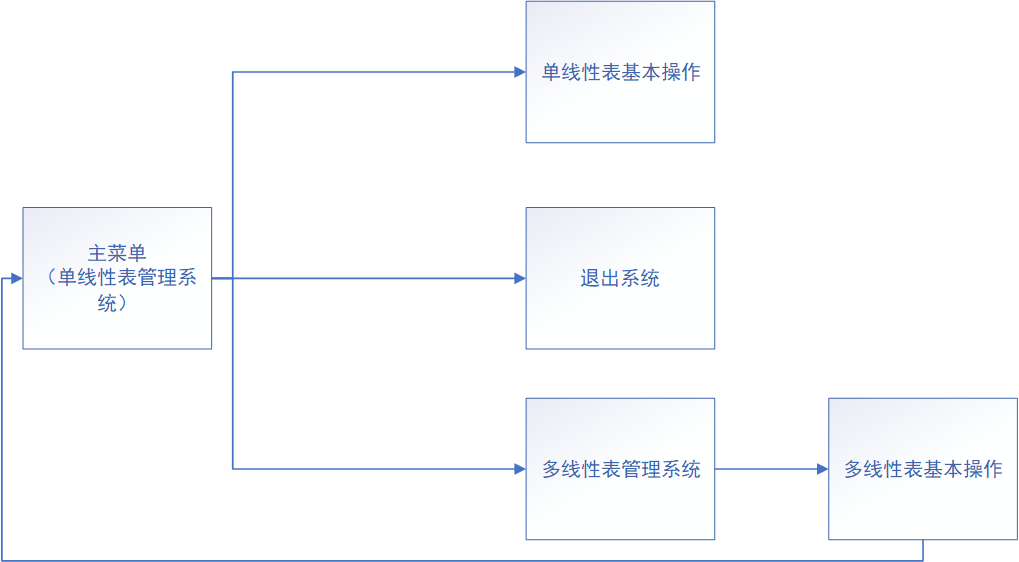
\includegraphics[width=1\linewidth]{images/2.1.png}
		\caption{演示系统模块结构图}
	\end{center}
\end{figure}
\subsubsection{ADT数据结构设计}
\noindent 对链表数据类型的定义如下\par
\begin{lstlisting}[language=C] 
typedef int status;//状态定义 
typedef int ElemType; //数据元素类型定义
typedef struct LNode
{  //单链表(链式结构)结点的定义
	ElemType data;
	struct LNode *next;
}LNode,*LinkList;
\end{lstlisting}
对多线性表的存储数据结构定义如下:
\begin{lstlisting}
%typedef struct
{ // 线性表的管理表定义
	struct
	{
		char name[30];
		LinkList L;
	} elem[10];
	int length;
	int listsize;
} LISTS;
\end{lstlisting}
对一些常量的定义如下
\begin{lstlisting}[language=C] 
	#define LIST_INIT_SIZE 100
	#define LISTINCREMENT  10
	#define TRUE 1
	#define FALSE 0
	#define OK 1
	#define ERROR 0
	#define INFEASIBLE -1
	#define OVERFLOW -2
\end{lstlisting}


\subsection{系统实现}
\subsubsection{程序开发环境与语言}
PC操作系统为windows操作系统使用语言为C++。
\subsubsection{代码的组织结构}
演示系统以一个菜单作为交互界面,用户通过输入命令对应的编号来调用相应的函数来实现创建表,销毁表,清空表,插入元素,删除元素,求表长,判空表,求前驱,求后继,遍历链表等基本操作,以及保存为文件,加载文件,翻转链表,对链表排序、进入多线性表系统等进阶操作。
程序主函数为一个switch结构,根据输入的数字,执行不同的语句,进而调用不同的函数
单表交互界面如下图
\begin{figure}[H] % here top bottom
	\begin{center}
		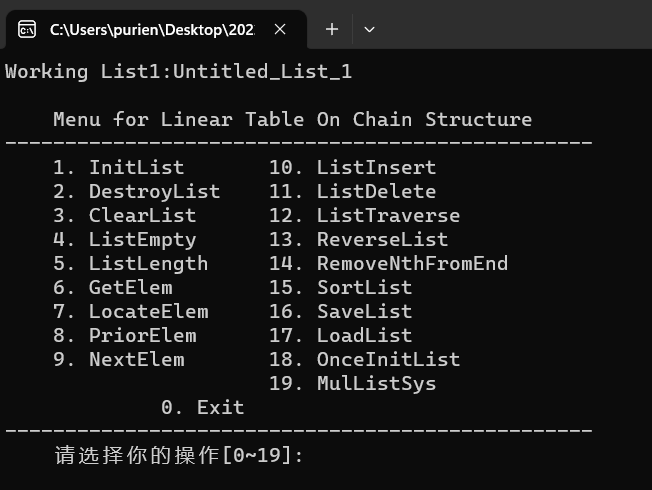
\includegraphics[width=0.7\linewidth]{images/1.3.1.png}
		\caption{单表交互界面示例}
	\end{center}
\end{figure}
输入19可进入多表交互界面,多表交互界面如下图
\begin{figure}[H] % here top bottom
	\begin{center}
		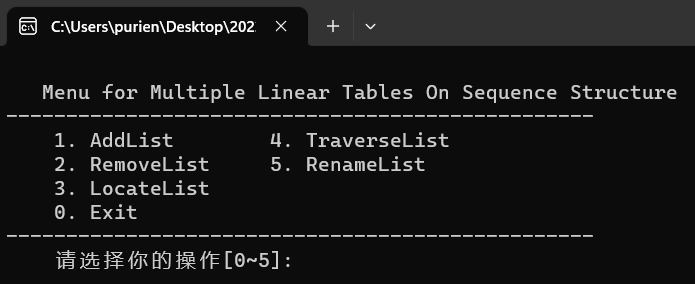
\includegraphics[width=0.7\linewidth]{images/1.3.2.png}
		\caption{多表交互界面示例}
	\end{center}
\end{figure}
\subsubsection{单链表基础运算算法实现}
\subsubsubsection{初始化表}
InitList(L):

----初始条件:线性表L不存在;

----操作结果:构造一个空的线性表;

算法的思想描述:为L结点分配存储空间,将L->next结点置空

算法处理步骤:
\begin{enumerate}
	\renewcommand{\labelenumi}{\theenumi)}
	\item 如果顺序表L不存在,则为L分配存储空间。
	\item 如果分配成功,将L->next置空返回状态OK。
	\item 如果分配失败,返回状态 OVERFLOW 并推出该程序块。
	\item 如果顺序表存在,返回状态 INFEASIBLE 以指出无法创建。
\end{enumerate}

时间复杂度:O(1)

空间复杂度:O(1)
\begin{figure}[H] % here top bottom
	\begin{center}
		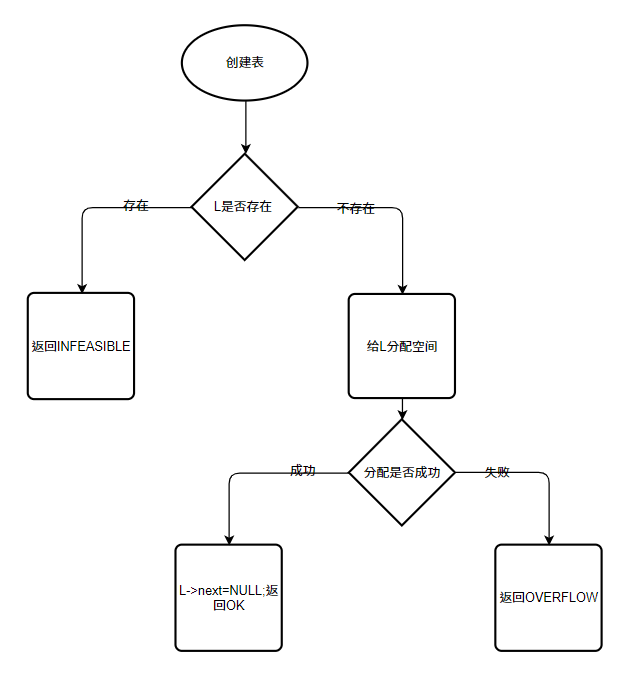
\includegraphics[width=0.8\linewidth]{images/1.2.3.png}
		\caption{初始化表流程图}
	\end{center}
\end{figure}
\subsubsubsection{销毁表}
DestroyList(L);

----初始条件:线性表L已存在;

----操作结果:销毁线性表L;

算法的思想描述:若 L 为 NULL,返回 INFEASIBLE。用 while 循环依次释放所有节点的储存空间,再将 L 置为 NULL。

时间复杂度:O(n)

空间复杂度:O(1)
\subsubsubsection{清空表}
ClearList(L);

----初始条件:线性表L已存在;

----操作结果:将L重置为空表;

算法的思想描述:若 L 为 NULL,返回 INFEASIBLE。\\否则用while循环释放除头节点以外的所有节点的储存空间,再将 L->next 置为 NULL。

时间复杂度:O(n)

空间复杂度:O(1)
\subsubsubsection{表判空}
ListEmpty(L);

----初始条件:线性表L已存在;

----操作结果:若L为空表则返回TRUE,否则返回FALSE;

算法的思想描述:若 L 为 NULL,返回 INFEASIBLE。否则判断 L->next 是否为 NULL,若为 NULL,则链表为空,否则链表不为空。

时间复杂度:O(1)

空间复杂度:O(1)
\subsubsubsection{求表长}

ListLength(L);

----初始条件:线性表已存在;

----操作结果:返回L中数据元素的个数;

算法思想描述:遍历整个顺序表

算法处理步骤:
\begin{enumerate}
	\renewcommand{\labelenumi}{\theenumi)}
	\item 如果顺序表L不存在,则输出INFEASIBLE。
	\item 如果L存在,从头开始遍历。
	\item 若不为空则移动指针到下一个结点,长度加1。
	\item 返回长度的值。
\end{enumerate}

时间复杂度:O(n)

空间复杂度:O(1)
\begin{figure}[H] % here top bottom
	\begin{center}
		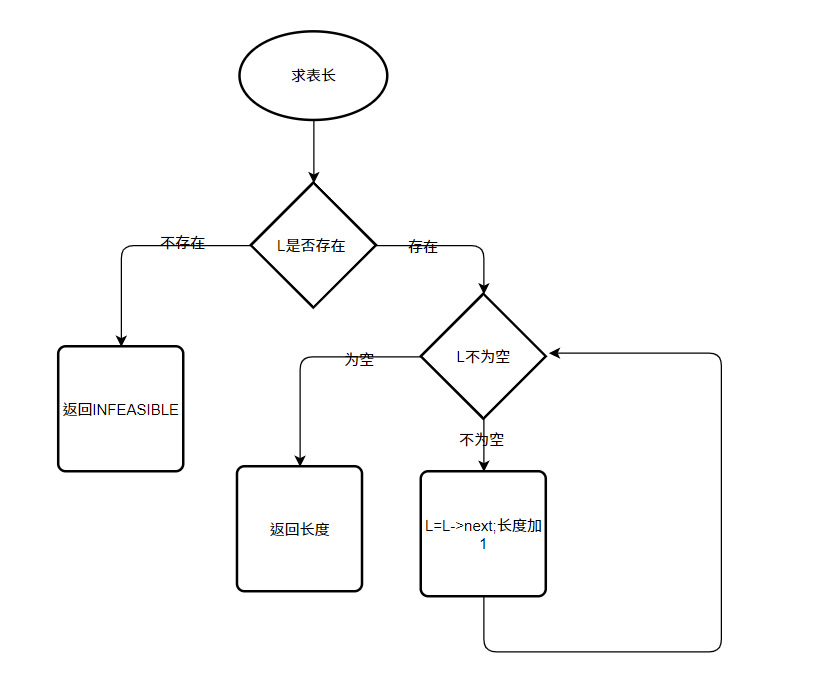
\includegraphics[width=0.8\linewidth]{images/1.2.4.png}
		\caption{求表长流程图}
	\end{center}
\end{figure}
\subsubsubsection{获取元素}
GetElem(L,i,e);

----初始条件:线性表已存在,1≤i≤ListLength(L);

----操作结果:用e返回L中第i个数据元素的值;

算法的思想描述:若 L 为 NULL,返回 INFEASIBLE。若 i 小于 1 或大于链表的长度,则该序号非法,返回 ERROR。否则遍历至第 i 个元素,返回其数据域的值。	

时间复杂度:O(n)

空间复杂度:O(1)
\subsubsubsection{定位元素}
LocateElem(L,e);

----初始条件:线性表已存在;

----操作结果:返回L中第1个与e相等的数据元素的位序,若这样的数据元素不存在,则返回值为0;

算法的思想描述:若 L 为 NULL,返回 INFEASIBLE。否则声明 i=0,遍历链表查找是
否有值与 e 相同的元素,每进入下一个节点时 i 自增,若找到相应元素则返回 i,
否则返回 ERROR。

时间复杂度:O(n)

空间复杂度:O(1)
\subsubsubsection{获得前驱}

PriorElem(L,cur\_e,pre\_e);

----初始条件:线性表L已存在;

----操作结果:若cur\_e是L的数据元素,且不是第一个,则用pre\_e返回它的前驱,否则操作失败,pre\_e无定义;

算法处理步骤:
\begin{enumerate}
	\renewcommand{\labelenumi}{\theenumi)}
	\item 如果顺序表L不存在,则输出INFEASIBLE。
	\item 如果L存在,从头开始遍历。
	\item 若当前节点的后继值为e,则将当前节点的值赋给pre,输出OK。
	\item 若为找到,则返回INFEASIBLE.
\end{enumerate}

时间复杂度:O(n)

空间复杂度:O(1)
\subsubsubsection{求后继}
NextElem(L,cur\_e,next\_e);

----初始条件:线性表L已存在;

----操作结果:若cur\_e是L的数据元素,且不是最后一个,则用next\_e返回它的后继,否则操作失败,next\_e无定义;

算法的思想描述:若 L 为 NULL,返回 INFEASIBLE。否则链表查找值等于 e 的元素,
若找到则将该节点后继节点的数据域赋值给 next,否则返回 ERROR。	

时间复杂度:O(n)

空间复杂度:O(1)
\subsubsubsection{插入元素}

ListInsert(L,i,e);

----初始条件:线性表L已存在,1≤i≤ListLength(L)+1;

----操作结果:在L的第i个位置之前插入新的数据元素e。

算法的思想描述:查找元素和移动之后的结点.

算法处理步骤:
\begin{enumerate}
	\renewcommand{\labelenumi}{\theenumi)}
	\item 如果顺序表L不存在,则输出INFEASIBLE。
	\item 如果L存在,判断i值是否符合要求,不符合则返回ERROR。
	\item 如果I值合法,增加一个新的结点用于存储插入元素。
	\item 将插入位置前的结点指向新插入的节点,将新节点指向插入位置后一个节点.
	\item 返回OK。
\end{enumerate}

时间复杂度:O(n)

空间复杂度:O(1)
\begin{figure}[H] % here top bottom
	\begin{center}
		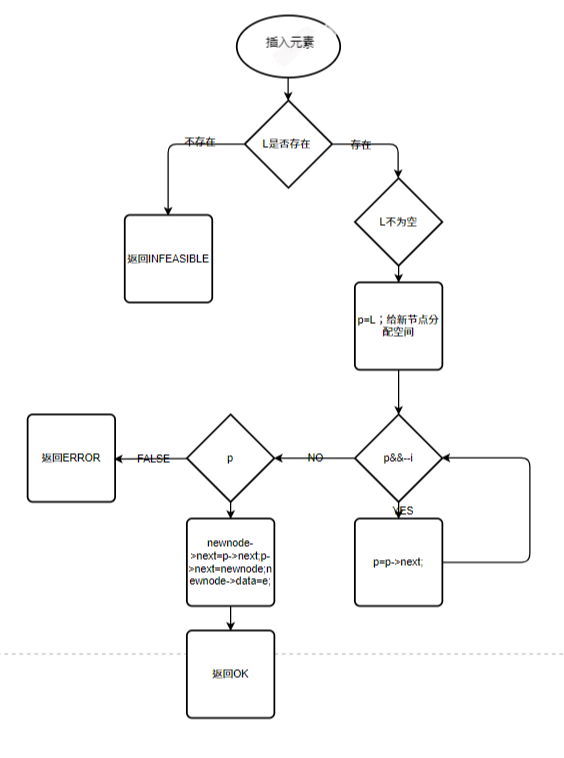
\includegraphics[width=0.8\linewidth]{images/1.2.6.png}
		\caption{插入元素流程图}
	\end{center}
\end{figure}
\subsubsubsection{删除元素}
ListDelete(L,i,e);

----初始条件:线性表L已存在且非空,1≤i≤ListLength(L);

----操作结果:删除L的第i个数据元素,用e返回其值;

算法的思想描述:若 L 为 NULL,返回 INFEASIBLE。若 i 小于 1 或大于链表长度则返回 ERROR。否则遍历至链表第 i-1 个元素,将其指针域置为其后继的后继,数据赋给 e,最后释放其后继节点。

时间复杂度:O(n)

空间复杂度:O(1)
\subsubsubsection{遍历链表}
ListTraverse(L,visit()),

----初始条件:线性表L已存在;

----操作结果:依次对L的每个数据元素调用函数visit()

算法思想描述:遍历链表并输出每一个元素的值.
\begin{enumerate}
	\renewcommand{\labelenumi}{\theenumi)}
	\item 如果顺序表L不存在,则输出INFEASIBLE。
	\item 如果L存在,从头开始遍历并输出。
	\item 返回OK。
\end{enumerate}

时间的复杂度:O(n).

空间的复杂度:O(1).
\subsubsubsection{链表的翻转} 

reverseList(L)

----初始条件:线性表L已存在;

----操作结果:将L翻转

算法的思想描述:遍历链表并存入数组,在数组中翻转并再次存入数组

算法处理的步骤:
\begin{enumerate}
	\renewcommand{\labelenumi}{\theenumi)}
	\item 如果L不存在则为空表,输出ERROR并退出.
	\item 建立一个新的节点,遍历所有节点以栈的形式存储
	\item 改变头节点为栈的头节点
\end{enumerate}

时间复杂度:O(n)

空间复杂度:O(n)
\subsubsubsection{删除链表的倒数第 n 个节点}
RemoveNthFromEnd(L,n)

----初始条件:线性表L已存在且非空;

----操作结果:删除该链表中倒数第n个节点

算法的思想描述:如果 L 为 NULL,返回 INFEASIBLE。否则调用求表长函数和删除节点函数,通过数学运算来实现倒数第 n 个元素的删除。	

时间复杂度:O(n)

空间复杂度:O(1)
\subsubsubsection{链表排序}
sortList(L)
----初始条件:线性表L已存在

----操作结果:将L升序排序

算法的思想描述:遍历链表将链表中元素存储到数组中,对数组进行冒泡排序,将排好的数组元素再次存入链表。

时间复杂度:O(n^2)

空间复杂度:O(n)
\subsubsubsection{读入文件}
SaveList(L,FileName)
----初始条件:线性表L已存在且非空;

----操作结果:将线性表L储存在名为FileName的文件中

算法的思想描述:若 L 为 NULL,返回 INFEASIBLE。打开文件,从文件中每读入一个数据创建一个节点,并置为上一个结点的后继,直到读取完所有数据,关闭文件。

时间复杂度:O(n)

空间复杂度:O(1)
\subsubsubsection{写入文件}
LoadList(L,FileName)
----初始条件:线性表L不存在;

----操作结果:将名为FileName的文件中内容存储到线性表L中

算法的思想描述:若 L 为 NULL,返回 INFEASIBLE。打开文件,遍历链表将所有元素的数据域写入文件,关闭文件。

时间复杂度:O(n)

空间复杂度:O(1)

\subsubsection{多线性表系统运算算法实现}
\subsubsubsection{添加线性表}
AddList(Lists, ListName)
----初始条件:多表Lists存在且未满;

----操作结果:在Lists中添加名为ListName的链表
算法的思想描述:若Lists未满,将ListName值拷贝给Lists中位置为Lists.size的链表元素的名称域,将链表头指针初始为空指针,并将Lists.size加1
时间复杂度为O(1)
空间复杂度为O(1)

\subsubsubsection{删除线性表}
RemoveList(Lists, ListName)
----初始条件:多表Lists存在,名为ListName的链表在Lists中存在

----操作结果:在Lists中删除名为ListName的链表
算法的思想描述:查找名为ListName的链表,将后续的链表元素向前移动1位,并将Lists.size减1
时间复杂度为O(n)
空间复杂度为O(1)
\subsubsubsection{查找线性表}
LocateList(Lists, ListName)
----初始条件:多表Lists存在,名为ListName的链表在Lists中存在

----操作结果:返回Lists中名为ListName的链表的逻辑序号,若不存在返回0
算法的思想描述:遍历Lists找到名称与ListName相同的链表
\subsubsubsection{遍历线性表}
TraverseList(Lists)
----初始条件:多表Lists存在

----操作结果:如果Lists中有线性表,依次显示线性表序号和名称,每个线性表占一行,并遍历每个线性表,返回OK;如果线性表Lists为空,返回ERROR。
\subsubsubsection{重命名线性表}
rename(Lists)
----初始条件:多表Lists存在,输入想修改的表的逻辑序号和重命名名称ListName,且序号名称合法

----操作结果:将该表重命名为ListName,若成功重命名,返回OK,若操作中断,返回ERROR 
\subsection{系统测试}
程序开发及实现环境:Win11 下使用 Dev C++ 进行编译和调试,开发语言为 C++ 语言。
测试数据:1 3 2 4 5
\subsubsection{单线性表系统测试}
\begin{enumerate}
	\renewcommand{\labelenumi}{\theenumi)}
	\item InitList和OnceInitList
	\begin{table}[h!]
		\begin{center}
			\caption{InitList函数测试}
			\begin{tabular}{|c|p{4cm}<{\centering}|p{4cm}<{\centering}|p{4cm}<{\centering}|} % <-- Alignments: 1st column left, 2nd middle and 3rd right, with vertical lines in between
				\hline
				\textbf{测试步骤} & \textbf{测试输入} & \textbf{理论结果} & \textbf{运行结果} \\
				\hline
				1 & 主界面输入1创建单链表 & 创建表时响应创建成功& 如图\ref{fig1-1-1}\\
				\hline
				2 & 再次创建单链表 & 显示线性表已存在 & 如图\ref{fig1-1-2}\\
				\hline
			\end{tabular}
		\end{center}
	\end{table}
	
	
	\begin{figure}[H] % here top bottom
		\begin{center}
			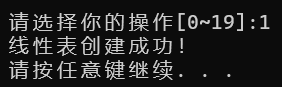
\includegraphics[width=0.5\linewidth]{images/linklist/1-1.png}
			\caption{InitList及Traverse函数测试}
			\label{fig1-1-1}
		\end{center}
	\end{figure}
	\begin{figure}[H] % here top bottom
		\begin{center}
			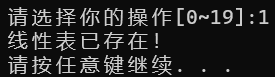
\includegraphics[width=0.5\linewidth]{images/linklist/1-2.png}
			\caption{InitList及Traverse函数测试}
			\label{fig1-1-2}
		\end{center}
	\end{figure}
	
	
	\item DestroyList
	\begin{table}[h!]
		\begin{center}
			\caption{DestroyList函数测试}
			\begin{tabular}{|c|p{4cm}<{\centering}|p{4cm}<{\centering}|p{4cm}<{\centering}|} 
				\hline
				\textbf{测试步骤} & \textbf{测试输入} & \textbf{理论结果} & \textbf{运行结果} \\
				\hline
				1 & 主界面输入2删除 & 显示删除成功 & 如图\ref{fig1-2-1}\\
				\hline
				2 & 主界面输入2删除 & 显示删除失败 & 如图\ref{fig1-2-2}\\
				\hline
			\end{tabular}
		\end{center}
	\end{table}
	
	
	\begin{figure}[H] % here top bottom
		\begin{center}
			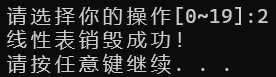
\includegraphics[width=0.5\linewidth]{images/linklist/2-1.png}
			\caption{DestroyList函数测试}
			\label{fig1-2-1}
		\end{center}
	\end{figure}
	\begin{figure}[H] % here top bottom
		\begin{center}
			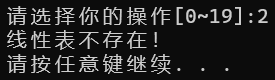
\includegraphics[width=0.5\linewidth]{images/linklist/2-2.png}
			\caption{DestroyList函数测试}
			\label{fig1-2-2}
		\end{center}
	\end{figure}
	
	\item ListEmpty和ClearList
	\begin{table}[h!]
		\begin{center}
			\caption{ListEmpty\&ClearList函数测试}
			\begin{tabular}{|c|p{4cm}<{\centering}|p{4cm}<{\centering}|p{4cm}<{\centering}|} 
				\hline
				\textbf{测试步骤} & \textbf{测试输入} & \textbf{理论结果} & \textbf{运行结果} \\
				\hline
				1 & 输入数据后主界面输入4 & 显示表不空 & 如图\ref{fig1-3-1}\\
				\hline
				2 & 清空表后再次判断 & 显示为空 & 如图\ref{fig1-3-2} \ref{fig1-3-3}\\
				\hline
			\end{tabular}
		\end{center}
	\end{table}
	
	
	\begin{figure}[H] % here top bottom
		\begin{center}
			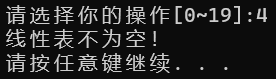
\includegraphics[width=0.5\linewidth]{images/linklist/4-2.png}
			\caption{ListEmpty\&ClearList函数测试}
			\label{fig1-3-1}
		\end{center}
	\end{figure}
	\begin{figure}[H] % here top bottom
		\begin{center}
			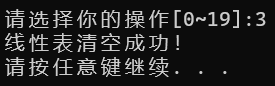
\includegraphics[width=0.5\linewidth]{images/linklist/3-1.png}
			\caption{ListEmpty\&ClearList函数测试}
			\label{fig1-3-2}
		\end{center}
	\end{figure}
	
	\begin{figure}[H] % here top bottom
		\begin{center}
			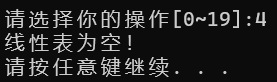
\includegraphics[width=0.5\linewidth]{images/linklist/4-1.png}
			\caption{ListEmpty\&ClearList函数测试}
			\label{fig1-3-3}
		\end{center}
	\end{figure}
	
	
	
	
	\item ListLenth
	
	\begin{table}[h!]
		\begin{center}
			\caption{ListLenth函数测试}
			\begin{tabular}{|c|p{4cm}<{\centering}|p{4cm}<{\centering}|p{4cm}<{\centering}|} 
				\hline
				\textbf{测试步骤} & \textbf{测试输入} & \textbf{理论结果} & \textbf{运行结果} \\
				\hline
				1 & 重新建立表1  主界面输入5求出表的长度 & 显示表长为5 & 如图\ref{fig1-4-1}\\
				\hline
				2 & 清空table1再次判断 & 显示长度为0 & 如图\ref{fig1-4-2}\\
				\hline
			\end{tabular}
		\end{center}
	\end{table}
	
	
	\begin{figure}[H] % here top bottom
		\begin{center}
			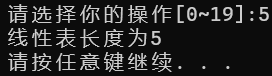
\includegraphics[width=0.5\linewidth]{images/linklist/5-2.png}
			\caption{ListLenth函数测试}
			\label{fig1-4-1}
		\end{center}
	\end{figure}
	
	
	\begin{figure}[H] % here top bottom
		\begin{center}
			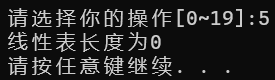
\includegraphics[width=0.5\linewidth]{images/linklist/5-1.png}
			\caption{ListLenth函数测试}
			\label{fig1-4-2}
		\end{center}
	\end{figure}
	
	
	\item GetElem
	\begin{table}[h!]
		\begin{center}
			\caption{GetElem函数测试}
			\begin{tabular}{|c|p{4cm}<{\centering}|p{4cm}<{\centering}|p{4cm}<{\centering}|} 
				\hline
				\textbf{测试步骤} & \textbf{测试输入} & \textbf{理论结果} & \textbf{运行结果} \\
				\hline
				1 &   主界面输入6并且输入2求第二个数 & 显示第二个数为3 & 如图\ref{fig1-5-1}\\
				\hline
				2 &   主界面输入6并且输入6求第六个数 & 显示不存在这个数 & 如图\ref{fig1-5-2}\\
				\hline
			\end{tabular}
		\end{center}
	\end{table}
	
	
	\begin{figure}[H] % here top bottom
		\begin{center}
			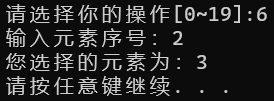
\includegraphics[width=0.5\linewidth]{images/linklist/6-1.png}
			\caption{GetElem函数测试}
			\label{fig1-5-1}
		\end{center}
	\end{figure}

	\begin{figure}[H] % here top bottom
	\begin{center}
		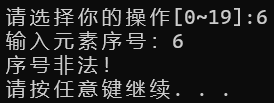
\includegraphics[width=0.5\linewidth]{images/linklist/6-2.png}
		\caption{GetElem函数测试}
		\label{fig1-5-2}
	\end{center}
	\end{figure}
	
	\item LocateElem
	\begin{table}[h!]
		\begin{center}
			\caption{LocateElem函数测试}
			\begin{tabular}{|c|p{4cm}<{\centering}|p{4cm}<{\centering}|p{4cm}<{\centering}|} 
				\hline
				\textbf{测试步骤} & \textbf{测试输入} & \textbf{理论结果} & \textbf{运行结果} \\
				\hline
				1正确数据测试 & 主界面输入7并且输入3进行查询 & 显示5序号为2 & 如图\ref{fig1-6-1}\\
				\hline
				2错误数据反馈 & 主界面输入7并且输入6进行查询 & 能够及时反馈不存在该数据 & 如图\ref{fig1-6-2}\\
				\hline
			\end{tabular}
		\end{center}
	\end{table}
	
	
	\begin{figure}[H] % here top bottom
		\begin{center}
			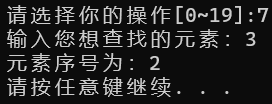
\includegraphics[width=0.5\linewidth]{images/linklist/7-1.png}
			\caption{LocateElem函数测试}
			\label{fig1-6-1}
		\end{center}
	\end{figure}
	
	\begin{figure}[H] % here top bottom
		\begin{center}
			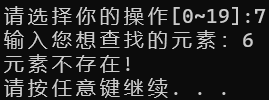
\includegraphics[width=0.5\linewidth]{images/linklist/7-2.png}
			\caption{LocateElem函数测试}
			\label{fig1-6-2}
		\end{center}
	\end{figure}
	
	
	\item PriorElem
	
	\begin{table}[h!]
		\begin{center}
			\caption{PriorElem函数测试}
			\begin{tabular}{|c|p{4cm}<{\centering}|p{4cm}<{\centering}|p{4cm}<{\centering}|} 
				\hline
				\textbf{测试步骤} & \textbf{测试输入} & \textbf{理论结果} & \textbf{运行结果} \\
				\hline
				1正确数据测试 & 主界面输入8并且输入3进行查询 & 显示5前驱为1 & 如图\ref{fig1-7-1}\\
				\hline
				2错误数据反馈 & 主界面输入8并且输入1进行查询 & 能够及时反馈不存在前驱 & 如图\ref{fig1-7-2}\\
				\hline
			\end{tabular}
		\end{center}
	\end{table}
	
	
	\begin{figure}[H] % here top bottom
		\begin{center}
			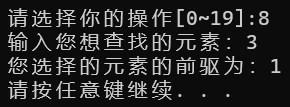
\includegraphics[width=0.5\linewidth]{images/linklist/8-1.png}
			\caption{PriorElem函数测试}
			\label{fig1-7-1}
		\end{center}
	\end{figure}
	
	\begin{figure}[H] % here top bottom
		\begin{center}
			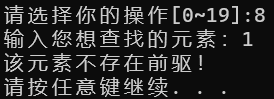
\includegraphics[width=0.5\linewidth]{images/linklist/8-2.png}
			\caption{PriorElem函数测试}
			\label{fig1-7-2}
		\end{center}
	\end{figure}
	
	\item NextElem
	
	\begin{table}[h!]
		\begin{center}
			\caption{NextElem函数测试}
			\begin{tabular}{|c|p{4cm}<{\centering}|p{4cm}<{\centering}|p{4cm}<{\centering}|} 
				\hline
				\textbf{测试步骤} & \textbf{测试输入} & \textbf{理论结果} & \textbf{运行结果} \\
				\hline
				1正确数据测试 & 主界面输入9并且输入2进行查询 & 显示5后继为4 & 如图\ref{fig1-8-1}\\
				\hline
				2错误数据反馈 & 主界面输入9并且输入5进行查询 & 能够及时反馈不存在后继 & 如图\ref{fig1-8-2}\\
				\hline
			\end{tabular}
		\end{center}
	\end{table}
	
	
	\begin{figure}[H] % here top bottom
		\begin{center}
			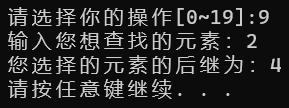
\includegraphics[width=0.5\linewidth]{images/linklist/9-1.png}
			\caption{NextElem函数测试}
			\label{fig1-8-1}
		\end{center}
	\end{figure}
	
	\begin{figure}[H] % here top bottom
		\begin{center}
			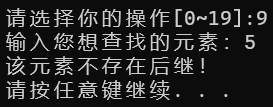
\includegraphics[scale=0.80]{images/linklist/9-2.png}
			\caption{NextElem函数测试}
			\label{fig1-8-2}
		\end{center}
	\end{figure}
	
	
	\item ListInsert
	
	\begin{table}[h!]
		\begin{center}
			\caption{ListInsert函数测试}
			\begin{tabular}{|c|p{4cm}<{\centering}|p{4cm}<{\centering}|p{4cm}<{\centering}|} 
				\hline
				\textbf{测试步骤} & \textbf{测试输入} & \textbf{理论结果} & \textbf{运行结果} \\
				\hline
				1 & 对table1在主界面输入10进行插入操作并输入数字6和位置6再遍历该表 & 显示table1中第一位插入18 & 如图\ref{fig1-9-1} \ref{fig1-9-2}\\
				\hline
				2 & 对table1在主界面输入10进行插入操作并输入数字6和位置10 & 显示插入失败 & 如图\ref{fig1-9-3}\\
				\hline
			\end{tabular}
		\end{center}
	\end{table}
	
	
	\begin{figure}[H] % here top bottom
		\begin{center}
			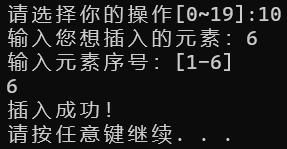
\includegraphics[width=0.5\linewidth]{images/linklist/10-1.png}
			\caption{ListInsert函数测试}
			\label{fig1-9-1}
		\end{center}
	\end{figure}
\begin{figure}[H] % here top bottom
	\begin{center}
		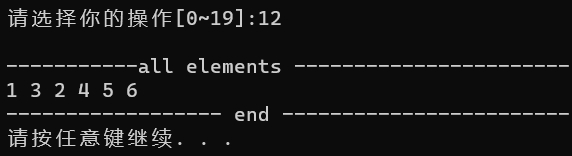
\includegraphics[width=0.5\linewidth]{images/linklist/10-12.png}
		\caption{ListInsert函数测试}
		\label{fig1-9-2}
	\end{center}
\end{figure}

\begin{figure}[H] % here top bottom
	\begin{center}
		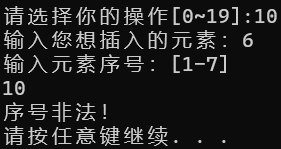
\includegraphics[width=0.5\linewidth]{images/linklist/10-2.png}
		\caption{ListInsert函数测试}
		\label{fig1-9-3}
	\end{center}
\end{figure}
	
	
	
	\item ListDelete
	
	\begin{table}[h!]
		\begin{center}
			\caption{ListDelete函数测试}
			\begin{tabular}{|c|p{4cm}<{\centering}|p{4cm}<{\centering}|p{4cm}<{\centering}|} 
				\hline
				\textbf{测试步骤} & \textbf{测试输入} & \textbf{理论结果} & \textbf{运行结果} \\
				\hline
				1正确操作 & 对刚刚进行过插入操作的线性表进行删除第六个数据的操作 & 显示已经顺利删除 & 如图\ref{fig1-10-1}\\
				\hline
				2验证正确性操作 & 选择遍历并验证是否与未插入时一致 & 显示对应数据 & 如图\ref{fig1-10-2}\\
				\hline
				3错误操作 & 删除第八个数据的操作 & 显示删除失败 & 如图\ref{fig1-10-3}\\
				\hline
			\end{tabular}
		\end{center}
	\end{table}
	
	
	\begin{figure}[H] % here top bottom
		\begin{center}
			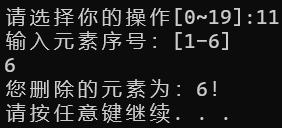
\includegraphics[width=0.5\linewidth]{images/linklist/11-1.png}
			\caption{ListDelete函数测试}
			\label{fig1-10-1}
		\end{center}
	\end{figure}
	
	\begin{figure}[H] % here top bottom
		\begin{center}
			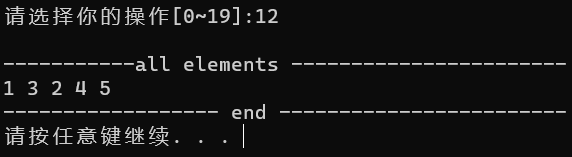
\includegraphics[width=0.5\linewidth]{images/linklist/12-1.png}
			\caption{ListDelete函数测试}
			\label{fig1-10-2}
		\end{center}
	\end{figure}
	
	\begin{figure}[H] % here top bottom
		\begin{center}
			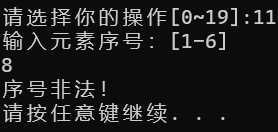
\includegraphics[width=0.5\linewidth]{images/linklist/11-2.png}
			\caption{ListDelete函数测试}
			\label{fig1-10-3}
		\end{center}
	\end{figure}
	
	
	\item TraverseList
	
	\begin{table}[h!]
		\begin{center}
			\caption{ TraverseList函数测试}
			\begin{tabular}{|c|p{4cm}<{\centering}|p{4cm}<{\centering}|p{4cm}<{\centering}|} 
				\hline
				\textbf{测试步骤} & \textbf{测试输入} & \textbf{理论结果} & \textbf{运行结果} \\
				\hline
				1 & 在主界面输入13翻转链表 & 显示翻转成功 & 如图\ref{fig1-11-1}\\
				\hline
				2 & 在主界面输入12遍历链表 & 显示翻转后数据 & 如图\ref{fig1-11-2}\\
				\hline
			\end{tabular}
		\end{center}
	\end{table}
	
	
	\begin{figure}[H] % here top bottom
		\begin{center}
			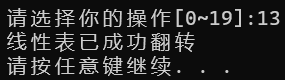
\includegraphics[width=0.5\linewidth]{images/linklist/13-1.png}
			\caption{ TraverseList函数测试}
			\label{fig1-11-1}
		\end{center}
	\end{figure}

	\begin{figure}[H] % here top bottom
		\begin{center}
			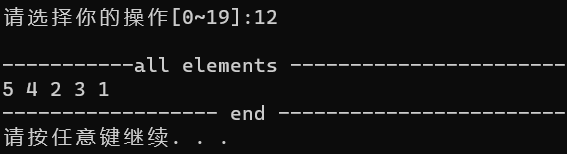
\includegraphics[width=0.5\linewidth]{images/linklist/13-12.png}
			\caption{ TraverseList函数测试}
			\label{fig1-11-2}
		\end{center}
	\end{figure}
	
	\item RemoveNthFromEnd
	
	\begin{table}[h!]
		\begin{center}
			\caption{ RemoveNthFromEnd函数测试}
			\begin{tabular}{|c|p{4cm}<{\centering}|p{4cm}<{\centering}|p{4cm}<{\centering}|} 
				\hline
				\textbf{测试步骤} & \textbf{测试输入} & \textbf{理论结果} & \textbf{运行结果} \\
				\hline
				1 & 对table1在主界面输入14并删除倒数第二个结点 & 显示删除4 & 如图\ref{fig1-12-1}\\
				\hline
				2 & 对table1在主界面输入12遍历链表 & 显示删除4后的数据 & 如图\ref{fig1-12-2}\\
				\hline
			\end{tabular}
		\end{center}
	\end{table}
	
	
	\begin{figure}[H] % here top bottom
		\begin{center}
			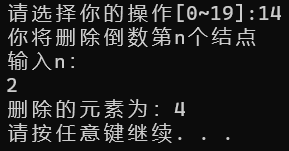
\includegraphics[width=0.5\linewidth]{images/linklist/14-1.png}
			\caption{ RemoveNthFromEnd函数测试}
			\label{fig1-12-1}
		\end{center}
	\end{figure}
	\begin{figure}[H] % here top bottom
		\begin{center}
			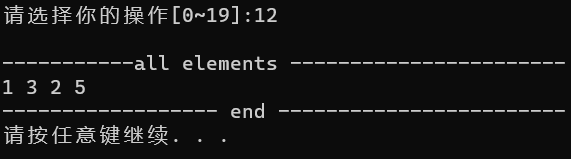
\includegraphics[width=0.5\linewidth]{images/linklist/14-12.png}
			\caption{ RemoveNthFromEnd函数测试}
			\label{fig1-12-2}
		\end{center}
	\end{figure}
	
	
	\item SortList
	\begin{table}[h!]
		\begin{center}
			\caption{SortList函数测试}
			\begin{tabular}{|c|p{4cm}<{\centering}|p{4cm}<{\centering}|p{4cm}<{\centering}|} 
				\hline
				\textbf{测试步骤} & \textbf{测试输入} & \textbf{理论结果} & \textbf{运行结果} \\
				\hline
				1 & 对table1在主界面输入15进行排序操作 & 显示已经排序完成 & 如图\ref{fig1-13-1}\\
				\hline
				2 & 对table1在主界面输入12遍历该线性表 & 输出数据为已经排序完成的一组数据 & 如图\ref{fig1-13-2}\\
				\hline
			\end{tabular}
		\end{center}
	\end{table}
	
	
	\begin{figure}[H] % here top bottom
		\begin{center}
			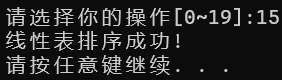
\includegraphics[width=0.5\linewidth]{images/linklist/15-1.png}
			\caption{ SortList函数测试}
			\label{fig1-13-1}
		\end{center}
	\end{figure}
	\begin{figure}[H] % here top bottom
		\begin{center}
			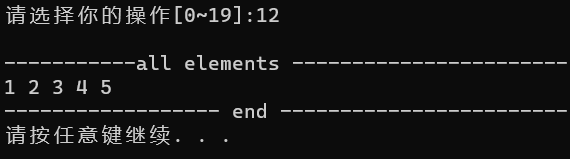
\includegraphics[width=0.5\linewidth]{images/linklist/15-12.png}
			\caption{ SortList函数测试}
			\label{fig1-13-2}
		\end{center}
	\end{figure}
	\item SaveList
	
	\begin{table}[h!]
		\begin{center}
			\caption{SaveList函数测试}
			\begin{tabular}{|c|p{4cm}<{\centering}|p{4cm}<{\centering}|p{4cm}<{\centering}|} 
				\hline
				\textbf{测试步骤} & \textbf{测试输入} & \textbf{理论结果} & \textbf{运行结果} \\
				\hline
				1&主界面输入16将该线性表保存到名为test.txt的文件中并打开文件查看内容 &文件里包含线性表元素 &如图\ref{fig1-14-1}和\ref{fig1-14-2} \\
				\hline
			\end{tabular}
		\end{center}
	\end{table}
	
	
	\begin{figure}[H] % here top bottom
		\begin{center}
			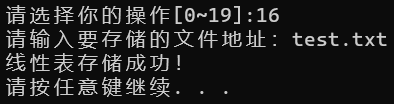
\includegraphics[width=0.5\linewidth]{images/linklist/16-1.png}
			\caption{ SaveList函数测试}
			\label{fig1-14-1}
		\end{center}
	\end{figure}
	
	
	\begin{figure}[H] % here top bottom
		\begin{center}
			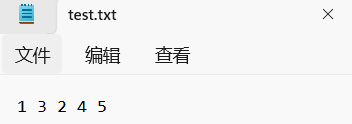
\includegraphics[width=0.5\linewidth]{images/linklist/16-2.png}
			\caption{ SaveList 函数测试}
			\label{fig1-14-2}
		\end{center}
	\end{figure}
	
	
	\item LoadList
	
	\begin{table}[h!]
		\begin{center}
			\caption{LoadList函数测试}
			\begin{tabular}{|c|p{4cm}<{\centering}|p{4cm}<{\centering}|p{4cm}<{\centering}|} 
				\hline
				\textbf{测试步骤} & \textbf{测试输入} & \textbf{理论结果} & \textbf{运行结果} \\
				\hline
				1正确操作 & 新建一个线性表命名为table2并在操作中选择17将test.txt文件读入table2中在遍历table2 &table2中包含table1的元素 &如图\ref{fig1-15-1}和\ref{fig1-15-2}\\
				\hline
				2错误操作 & 对已存在的线性表进行上述操作 &显示线性表已存在 &如图\ref{fig1-15-3}\\
				\hline
				3错误操作 & 对不存在的线性表进行上述操作,但文件名改为text.txt &显示文件读取失败 &如图\ref{fig1-15-4}\\
				\hline
			\end{tabular}
		\end{center}
	\end{table}
	
	
	\begin{figure}[H] % here top bottom
		\begin{center}
			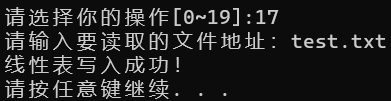
\includegraphics[width=0.5\linewidth]{images/linklist/17-1.png}
			\caption{ LoadList函数测试}
			\label{fig1-15-1}
		\end{center}
	\end{figure}
	\begin{figure}[H] % here top bottom
		\begin{center}
			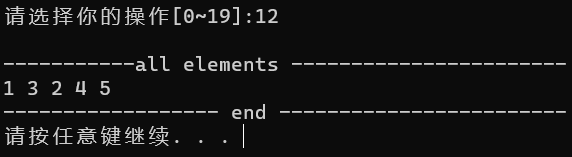
\includegraphics[width=0.5\linewidth]{images/linklist/12-1.png}
			\caption{ LoadList函数测试}
			\label{fig1-15-2}
		\end{center}
	\end{figure}
	\begin{figure}[H] % here top bottom
		\begin{center}
			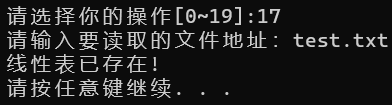
\includegraphics[width=0.5\linewidth]{images/linklist/17-2.png}
			\caption{ LoadList函数测试}
			\label{fig1-15-3}
		\end{center}
	\end{figure}
	\begin{figure}[H] % here top bottom
		\begin{center}
			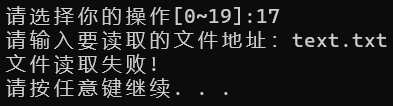
\includegraphics[width=0.5\linewidth]{images/linklist/17-3.png}
			\caption{ LoadList函数测试}
			\label{fig1-15-4}
		\end{center}
	\end{figure}
\subsubsection{多线性表系统测试}
	\item AddList
	\begin{table}[h!]
		\begin{center}
			\caption{AddList函数测试}
			\begin{tabular}{|c|p{4cm}<{\centering}|p{4cm}<{\centering}|p{4cm}<{\centering}|} 
				\hline
				\textbf{测试步骤} & \textbf{测试输入} & \textbf{理论结果} & \textbf{运行结果} \\
				\hline
				1正确操作 & 新建两个分别名为list1,list2的线性表 &创建成功 &如图\ref{fig1-16-1}和\ref{fig1-16-2}\\
				\hline
				2错误操作 & 再新建一个名为list2的线性表 &显示名称重复 &如图\ref{fig1-16-3}\\
				\hline
				3 & 遍历多线性表管理系统 &显示现在存在的线性表 &如图\ref{fig1-16-4}\\
				\hline
			\end{tabular}
		\end{center}
	\end{table}
	\begin{figure}[H] % here top bottom
		\begin{center}
			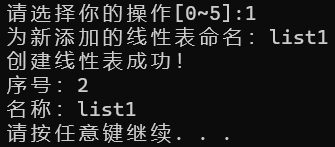
\includegraphics[width=0.5\linewidth]{images/linklist/19-1-1.png}
			\caption{ AddList函数测试}
			\label{fig1-16-1}
		\end{center}
	\end{figure}
\begin{figure}[H] % here top bottom
	\begin{center}
		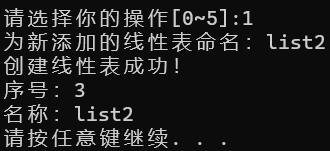
\includegraphics[width=0.5\linewidth]{images/linklist/19-1-3.png}
		\caption{ AddList函数测试}
		\label{fig1-16-2}
	\end{center}
\end{figure}
\begin{figure}[H] % here top bottom
	\begin{center}
		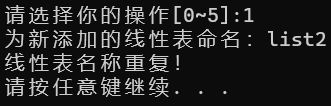
\includegraphics[width=0.5\linewidth]{images/linklist/19-1-2.png}
		\caption{ AddList函数测试}
		\label{fig1-16-3}
	\end{center}
\end{figure}
\begin{figure}[H] % here top bottom
	\begin{center}
		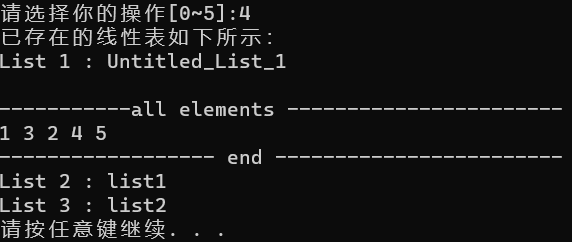
\includegraphics[width=0.5\linewidth]{images/linklist/19-4-1.png}
		\caption{ AddList函数测试}
		\label{fig1-16-4}
	\end{center}
\end{figure}

	\item RemoveList
	\begin{table}[h!]
		\begin{center}
			\caption{RemoveList函数测试}
			\begin{tabular}{|c|p{4cm}<{\centering}|p{4cm}<{\centering}|p{4cm}<{\centering}|} 
				\hline
				\textbf{测试步骤} & \textbf{测试输入} & \textbf{理论结果} & \textbf{运行结果} \\
				\hline
				1正确操作 & 删除名为list1的线性表 &显示删除成功 &如图\ref{fig1-17-1}\\
				\hline
				2错误操作 & 再删除名为list1的线性表 &显示线性表不存在 &如图\ref{fig1-17-2}\\
				\hline
				3 & 遍历多线性表管理系统 &显示现在存在的线性表 &如图\ref{fig1-17-3}\\
				\hline
			\end{tabular}
		\end{center}
	\end{table}
	\begin{figure}[H] % here top bottom
		\begin{center}
			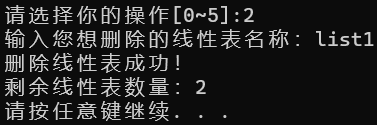
\includegraphics[width=0.5\linewidth]{images/linklist/19-2-1.png}
			\caption{ RemoveList函数测试}
			\label{fig1-17-1}
		\end{center}
	\end{figure}
	\begin{figure}[H] % here top bottom
		\begin{center}
			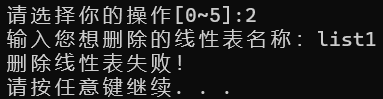
\includegraphics[width=0.5\linewidth]{images/linklist/19-2-2.png}
			\caption{ RemoveList函数测试}
			\label{fig1-17-2}
		\end{center}
	\end{figure}
	\begin{figure}[H] % here top bottom
		\begin{center}
			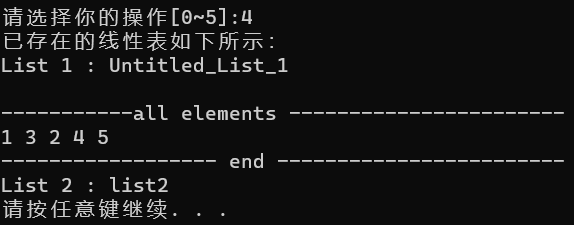
\includegraphics[width=0.5\linewidth]{images/linklist/19-2-4.png}
			\caption{ RemoveList函数测试}
			\label{fig1-17-3}
		\end{center}
	\end{figure}

	\item LocateList
	\begin{table}[h!]
		\begin{center}
			\caption{LocateList函数测试}
			\begin{tabular}{|c|p{4cm}<{\centering}|p{4cm}<{\centering}|p{4cm}<{\centering}|} 
				\hline
				\textbf{测试步骤} & \textbf{测试输入} & \textbf{理论结果} & \textbf{运行结果} \\
				\hline
				1正确操作 & 查找名为list2的线性表 &显示该线性表序号为2 &如图\ref{fig1-18-1}\\
				\hline
				2错误操作 & 查找名为list1的线性表 &显示线性表不存在 &如图\ref{fig1-18-2}\\
				\hline
			\end{tabular}
		\end{center}
	\end{table}
	\begin{figure}[H] % here top bottom
		\begin{center}
			\includegraphics[width=0.5\linewidth]{images/linklist/19-3-1.png}
			\caption{ LocateList函数测试}
			\label{fig1-18-1}
		\end{center}
	\end{figure}
\begin{figure}[H] % here top bottom
	\begin{center}
		\includegraphics[width=0.5\linewidth]{images/linklist/19-3-2.png}
		\caption{ LocateList函数测试}
		\label{fig1-18-2}
	\end{center}
\end{figure}
	\item TraverseList
	\begin{table}[h!]
		\begin{center}
			\caption{TraverseList函数测试}
			\begin{tabular}{|c|p{4cm}<{\centering}|p{4cm}<{\centering}|p{4cm}<{\centering}|} 
				\hline
				\textbf{测试步骤} & \textbf{测试输入} & \textbf{理论结果} & \textbf{运行结果} \\
				\hline
				1 & 遍历多线性表系统 &显示此时的线性表 &如图\ref{fig1-19-1}\\
				\hline
				2 & 将数据输入list2线性表并再次遍历 &显示此时线性表&如图\ref{fig1-19-2}\\
				\hline
			\end{tabular}
		\end{center}
	\end{table}
	\begin{figure}[H] % here top bottom
		\begin{center}
			\includegraphics[width=0.5\linewidth]{images/linklist/19-2-4.png}
			\caption{ TraverseList函数测试}
			\label{fig1-19-1}
		\end{center}
	\end{figure}
	\begin{figure}[H] % here top bottom
		\begin{center}
			\includegraphics[width=0.5\linewidth]{images/linklist/19-4.png}
			\caption{ TraverseList函数测试}
			\label{fig1-19-2}
		\end{center}
	\end{figure}
	\item RenameList
	\begin{table}[h!]
		\begin{center}
			\caption{RenameList函数测试}
			\begin{tabular}{|c|p{4cm}<{\centering}|p{4cm}<{\centering}|p{4cm}<{\centering}|} 
				\hline
				\textbf{测试步骤} & \textbf{测试输入} & \textbf{理论结果} & \textbf{运行结果} \\
				\hline
				1 & 输入5修改序号为2的名称为abc &名称修改成功 &如图\ref{fig1-20-1}\\
				\hline
				2 & 遍历多线性表 &list2已改名为abc &如图\ref{fig1-20-2}\\
				\hline
			\end{tabular}
		\end{center}
	\end{table}
	\begin{figure}[H] % here top bottom
		\begin{center}
			\includegraphics[width=0.5\linewidth]{images/linklist/19-5.png}
			\caption{ RenameList函数测试}
			\label{fig1-20-1}
		\end{center}
	\end{figure}
\begin{figure}[H] % here top bottom
	\begin{center}
		\includegraphics[width=0.5\linewidth]{images/linklist/19-5-4.png}
		\caption{ RenameList函数测试}
		\label{fig1-20-2}
	\end{center}
\end{figure}
\end{enumerate}

\quad 通过异常用例可以看出,演示系统对表不存在时对除创建表以外的操作和对查找表中没有的元素的前驱、后继或对无后继、无前驱的元素要求获取后继、前驱的操作,以及在表存在时要求读取文件的操作的判定能力,可见演示系统能够识别异常样例。

\subsection{实验小结}
实验中遇到的问题和对应解决方案如下:\par
\subsubsection{无法第二次进入多表系统}
问题描述:在进入多表系统进行多表操作后,退回单表系统,之后再次输入19进入多表系统却失败。\par

原因分析:检查后发现我的多表系统仿照单表系统设置了一个int变量OP,其值为每次输入的操作号,对于单表来说,操作号为0即程序终止,但对多表来说只是退出了多表系统,若不及时重置该int值,当再次进入多表系统时其值为0就会自动退出。\par

解决方法:注意在退出多表系统后对OP进行初始化\par
\subsubsection{从多表系统进入单表系统后数据丢失}
	问题描述:在单表存储数据,进入多表系统中发现数据不见了。\par
	原因分析:每次退出多表系统时,我会将用户选择操作的单表的头节点指针赋给指针p并在接下来对p进行操作,当p不为空时当然可行,但是在多表系统中新创建的线性表头节点初始化为空指针,在单表系统中才对其分配空间,分配空间会改变头节点指针的值,而多表的结构体中头节点指针值并没有改变,依然为空指针。\par
	问题解决:放弃了将结构体相应头节点指针赋值给p的操作,定义一个int变量now对应现在操作的单表在多表结构体中的序号,在每次操作时都是直接对多表结构体中相应头节点进行操作。\par
	
\clearpage

\section{基于邻接表的图实现}
\subsection{问题描述}
\noindent 实验要求:
\begin{enumerate}
	\item 实现对图的基本操作;
	\item 选择性实践对图的进阶操作;
	\item 设计演示系统。
\end{enumerate}
通过实验达到:
\begin{enumerate}
	\item 加深对图的概念、基本运算的理解;	
	\item 熟练掌握图的逻辑结构与物理结构的关系;
	\item 以邻接表作为物理结构,熟练掌握图基本运算的实现。
\end{enumerate}
分析:需要了解图的结构,同时演示系统要清晰明了。

\subsection{系统设计}

\subsubsection{演示系统菜单的组织架构}
\quad 演示系统分为基本操作和进阶操作两部分,以一个菜单为主界面,以序号1至12表示创建,销毁,清空,插入,删除,遍历等基本操作,以序号13至17表示保存为文件,求最短通路,求距某顶点距离小于d的顶点,对顶点进行修改等进阶操作,以序号0表示退出演示系统,根据序号调用函数执行操作。
演示系统模块结构图如下
\begin{figure}[H] % here top bottom
	\begin{center}
		\includegraphics[width=1\linewidth]{images/2.3.png}
		\caption{演示系统模块结构图}
	\end{center}
\end{figure}
\subsubsection{ADT数据结构设计}
\noindent 对图数据类型的定义如下\par
\begin{lstlisting}[language=C] 
typedef struct {
	KeyType  key;
	char others[20];
} VertexType; //顶点类型定义


typedef struct ArcNode {//表结点类型定义
	int adjvex;//顶点位置编号 
	struct ArcNode  *nextarc;//下一个表结点指针
} ArcNode;
typedef struct VNode{//头结点及其数组类型定义
	VertexType data;//顶点信息
	ArcNode *firstarc;//指向第一条弧
} VNode,AdjList[MAX_VERTEX_NUM];

typedef  struct {//邻接表的类型定义
	AdjList vertices;//头结点数组
	int vexnum,arcnum;//顶点数、弧数
	GraphKind  kind;//图的类型
} ALGraph;
\end{lstlisting}
对多图管理系统的定义如下:
\begin{lstlisting}[language=C] 
typedef struct 
{//多图管理的定义 
	struct
	{
		char name[30];
		ALGraph G;
	} elem[20];
	int length; //图的总数 
	int size;//图的最大数目 
} ALGRAPHS; 
\end{lstlisting}
对一些常量的定义如下:
\begin{lstlisting}[language=C] 
	#define TRUE 1
	#define FALSE 0
	#define OK 1
	#define ERROR 0
	#define INFEASIBLE -1
	#define OVERFLOW -2
	#define MAX_VERTEX_NUM 20
\end{lstlisting}


\newpage 
\subsection{系统实现}
\subsubsection{程序开发环境与语言}
PC操作系统为windows操作系统使用语言为C++。
\subsubsection{代码的组织结构}
演示系统以一个菜单作为交互界面,用户通过输入命令对应的编号来调用相应的函数来实现创建图,销毁图,清空图,插入顶点,删除顶点,遍历等基本操作,以及保存为文件,求最短通路,求距某顶点距离小于d的顶点,对顶点进行修改等进阶操作。
程序主函数为一个switch结构,根据输入的数字,执行不同的语句,进而调用不同的函数.
单图交互界面如下图
\begin{figure}[H] % here top bottom
	\begin{center}
		\includegraphics[width=0.8\linewidth]{images/2.3.1.png}
		\caption{单图交互界面示例}
	\end{center}
\end{figure}
输入19可进入多图交互界面,多图交互界面如下图
\begin{figure}[H] % here top bottom
	\begin{center}
		\includegraphics[width=0.8\linewidth]{images/2.3.8.png}
		\caption{多图交互界面示例}
	\end{center}
\end{figure}
\subsubsection{单图基础运算算法实现}
\subsubsubsection{创建图}
CreateCraph(\&G,V,VR);

----初始条件:V是图的顶点集,VR是图的关系集;

----操作结果:按V和VR的定义构造图G。

算法的思想描述:定义 vexnum=0,arcnum=0,分别记录顶点和边的数目。
如若当前顶点序列的关键字不为-1 执行 while 循环:如果当前关键字未出现
则更新标记数组并继续,否则返回 ERROR,在邻接表添加新顶点,令表头
结点为 NULL,更新顶点数,检查是否超过最大数目MAXVERTEXNUM ,超过则返回 ERROR。
循环结束如果vexnum=0,即没有顶点,则返回ERROR,否则令G.vexnum=vexnum。
当当前关系序列不为 (-1,-1) 时执行 while 循环:用 for 循环遍历邻接表,查
找关系序列相应顶点

算法的思想描述:若 L 为 NULL,返回 INFEASIBLE。用 while 循环依次释放所有节点的储存空间,再将 L 置为 NULL。

时间复杂度:O(n)

空间复杂度:O(n)


\subsubsubsection{销毁图}

DestroyBiTree(T);

----初始条件:图G已存在;

----操作结果:销毁图G。

算法的思想描述:遍历所有弧结点

算法处理步骤:
\begin{enumerate}
	\renewcommand{\labelenumi}{\theenumi)}
	\item 用两个临时变量分别记录首节点与下一结点。
	\item 删除首个顶点然后两个结点开始移动,遍历完一个顶点的所有邻接点。
	\item 重复直至所有结点都遍历过。
	\item 删除成功,返回 OK。
\end{enumerate}

时间复杂度:O(n)

空间复杂度:O(1)
\begin{figure}[H] % here top bottom
	\begin{center}
		\includegraphics[width=0.8\linewidth]{images/2.3.2.png}
		\caption{销毁表流程图}
	\end{center}
\end{figure}
\subsubsubsection{查找顶点}
LocateVex(G,u);

----初始条件:图G存在,u和G中的顶点具有相同特征;

----操作结果:若u在图G中存在,返回顶点u的位置信息,否则返回其它信息。

算法的思想描述:用 for 循环遍历邻接表,如果当前顶点关键字与所找关键字相等,则返回当前顶点序号。如果没找到,返回-1。

时间复杂度:O(n)

空间复杂度:O(1)
\subsubsubsection{顶点赋值}
PutVex (G,u,value);

----初始条件:图G存在,u是和G中顶点关键字类型相同的给定值;

----操作结果:对关键字为u的顶点赋值value。

算法的思想描述:寻找赋值顶点并赋值

算法处理步骤:
\begin{enumerate}
	\renewcommand{\labelenumi}{\theenumi)}
	\item 定位需要赋值的顶点的位置。
	\item 将该顶点的关键字和值域重新赋值。
	\item 修改成功,返回 OK。
\end{enumerate}

时间复杂度:O(n)

空间复杂度:O(1)
\subsubsubsection{第一邻接点}
FirstAdjVex(G, u)
----初始条件:图G存在,u是G中顶点的位序

----操作结果:返回u对应顶点的第一个邻接顶点位序,如果u的顶点没有邻接顶点,否则返回其它表示“不存在”的信息。

算法思想描述:调用定位函数查找关键字为u的结点。如果 i == G.vexnum || G.vertices[i].firstarc == NULL,即没找到该点或该点无
邻接点,则返回-1。否则返回 G.vertices[i].firstarc->adjvex。

算法处理步骤:
\begin{enumerate}
	\renewcommand{\labelenumi}{\theenumi)}
	\item 定位关键字为 v 的顶点的位置.
	\item 若下一个弧结点不为空则返回它否则返回-1。
\end{enumerate}

时间复杂度:O(n)

空间复杂度:O(1)
\subsubsubsection{下一邻接点}

NextAdjVex(G, v, w)
----初始条件:图G存在,v和w是G中两个顶点的位序,v对应G的一个顶点,w对应v的邻接顶点

----操作结果:返回v的(相对于w)下一个邻接顶点的位序,如果w是最后一个邻接顶点,返回其它表示“不存在”的信息。

算法的思想描述:调用定位函数查找关键字为u的结点。如果 i==G.vexnum,返回ERROR。用 while 循环遍历该顶点的所有邻接点,找到另个一顶点,用 p 指向该邻接点。如果 p == NULL || p->nextarc == NULL,即 v 与 w 不相邻,或 v 相对 w无下一邻接点,返回-1。否则返回 return p->nextarc->adjvex。

时间复杂度:O(n)

空间复杂度:O(1)
\subsubsubsection{插入顶点}
InsertVex(G,v)
----初始条件:图G存在,v和G中的顶点具有相同特征

----操作结果:在图G中增加新顶点v,并保持顶点关键字的唯一性。

算法的思想描述:如果 G.vexnum == MAXVERTEXNUM,返回 ERROR。如若不然使用 LocateVex 查找要插入结点的关键字。如果要插入顶点的关键字已出现,则返回 ERROR。否则插入新顶点,更新顶点数,返回 OK。

时间复杂度:O(n)

空间复杂度:O(1)

\subsubsubsection{删除顶点}

DeleteVex(G,v)
----初始条件:图G存在,v是和G中顶点关键字类型相同的给定值

----操作结果:在图G中删除关键字v对应的顶点以及相关的弧

算法思想的描述:寻找所要删除的顶点,记录它所连接的所有弧结点 ,在其他顶点中将所有的弧结点删除


时间复杂度:O(n*n)

空间复杂度:O(1)
\subsubsubsection{插入弧}
InsertArc(G,v,w)
----初始条件:图G存在,v、w是和G中顶点关键字类型相同的给定值

----操作结果:在图G中增加弧<v,w>,如果图G是无向图,还需要增加<w,v>

算法的思想描述:查找 v,w 的关键字,如果其中任意一个未找到,则返回 ERROR,否则分别在这两个关键字后的链表中添加相应弧,返回 OK。	
算法处理步骤:
\begin{enumerate}
	\renewcommand{\labelenumi}{\theenumi)}
	\item 寻找所要插入的结点 v,w
	\item 在 v 和 w 中分别用首插法
	\item 总弧数加 1 。
\end{enumerate}

时间复杂度:O(n)

空间复杂度:O(1)
\begin{figure}[H] % here top bottom
	\begin{center}
		\includegraphics[width=0.8\linewidth]{images/2.3.5.png}
		\caption{插入弧流程图}
	\end{center}
\end{figure}
\subsubsubsection{删除弧}
DeleteArc(G,v,w)

----初始条件:图G存在,v、w是和G中顶点关键字类型相同的给定值

----操作结果:在图G中删除弧<v,w>,如果图G是无向图,还需要删除<w,v>

算法的思想描述:调用函数查找 v,w 的关键字,如果其中任意一个未找到,则返回 ERROR,否则分别在这两个关键字后的链表中寻找并删除对应结点的弧,返回 OK。	

算法处理步骤:
\begin{enumerate}
	\renewcommand{\labelenumi}{\theenumi)}
	\item 寻找所要删除的弧的信息。
	\item 分别在 v 中删除 w 和在 w 中删除 v。
	\item 若删除成功则返回 OK。
\end{enumerate}

时间复杂度:O(n)

空间复杂度:O(1)
\subsubsubsection{深度优先遍历}
DFSTraverse(G,visit())
----初始条件:图G存在

----操作结果:图G进行深度优先搜索遍历,依次对图中的每一个顶点使用函数visit访问一次,且仅访问一次

算法的思想描述:如果 G.vexnum==0,即图不存在,返回 INFEASIBLE。定义标记数组用于标记顶点是否已访问;递归地从第一个顶点开始访问其余顶点,每次访问时更新标记数组,以确保每个节点只被访问一次;返回 OK。。
算法处理步骤:
\begin{enumerate}
	\renewcommand{\labelenumi}{\theenumi)}
	\item  构造一个对一个顶点所有邻接结点的递归函数fps
	\item  依次读取每个顶点并用标记数组记录已读取的顶点
	\item  用 visit 函数将深度遍历的结点信息逐个打印。
\end{enumerate}

时间复杂度:O(n+e)

空间复杂度:O(log n)
\subsubsubsection{广度优先遍历}
BFSTraverse(G,visit())
----初始条件:图G存在

----操作结果:图G进行广度优先搜索遍历,依次对图中的每一个顶点使用函数visit访问一次,且仅访问一次

算法思想描述:利用队列这一数据结构, 保存每一次广搜的所有弧结点并将他们在下一次广搜时访问所有未被读取的首节点。

时间的复杂度:O(n+e).

空间的复杂度:O(n).
\subsubsubsection{距离小于k的顶点集合}
VerticesSetLessThank(G,v,k);
----初始条件:图G存在,v为顶点

----操作结果:返回与顶点v距离小于k的顶点集合

\textbf{算法实现: }使用一个递归函数dfs(G,v,k)和visit数组用来记录是否访问过,函数dfs对其邻接的顶点u调用dfs(G,v.k-1),当k等于0时退出,此时访问过的顶点即为与顶点v距离小于k的顶点集合。

\textbf{时空效率: }时间复杂度为O(n+e),空间复杂度为O(n)。\\
\subsubsubsection{顶点间最短路径和长度}
ShortestPathLength(G,v,w);
----初始条件:图G存在,v为顶点

----操作结果:返回顶点v与顶点w的最短路径的长度

\textbf{算法实现: }使用Dijkstra算法,算出从v到w的最短路径

\textbf{时空效率: }时间复杂度为O($n^{2}$),空间复杂度为O(n)。\\
\subsubsubsection{计算图的联通分量}
ConnectedComponentsNums(G)
----初始条件:图G存在,v为顶点

----操作结果:返回图G的所有连通分量的个数

\textbf{算法实现: }定义count=0,对所有顶点进行dfs,dfs的起始顶点visit[i]==0时将count+1,全部dfs之后count的值即为连通分量个数

\textbf{时空效率: }时间复杂度为O($n^{2}$),空间复杂度为O(n)。\\
\subsubsubsection{图的文件存储}
SaveGraph(G,FileName)
----初始条件:图G存在

----操作结果:将图G的信息存储到名为FileName的文件中
\subsubsubsection{图的文件读取}
LoadGraph(G,FileName)
----初始条件:图G不存在

----操作结果:在名为FileName的文件中读取数据并存储到图G中
\subsubsection{多图系统运算算法实现}
\subsubsubsection{添加图}
AddGraph(Graphs, GraphName)
----初始条件:多图Graphs存在且未满;

----操作结果:在Graphs中添加名为GraphName的图
算法的思想描述:若Graphs未满,检查GraphName是否与已存在的图名称重复,若不重复,将GraphName值拷贝给Graphs中位置为Graphs.size的图的名称,初始化该图,并将Graphs.size加1
时间复杂度为O(n)
空间复杂度为O(1)

\subsubsubsection{删除图}
RemoveGraph(Graphs, GraphName)
----初始条件:多图Graphs存在,名为GraphName的图在Graphs中存在

----操作结果:在Graphs中删除名为GraphName的图
算法的思想描述:查找名为GraphName的图,将后续的图向前移动1位,并将Graphs.size减1
时间复杂度为O(n)
空间复杂度为O(1)
\subsubsubsection{查找图}
LocateGraph(Graphs, GraphName)
----初始条件:多图Graphs存在,名为GraphName的图在Graphs中存在

----操作结果:返回Graphs中名为GraphName的图的逻辑序号,若不存在返回0
算法的思想描述:遍历Graphs找到名称与GraphName相同的图
\subsubsubsection{遍历图}
TraverseGraph(Graphs)
----初始条件:多表Graphs存在

----操作结果:如果Graphs中有图,依次显示图序号和名称,每个图占一行,并遍历每个图(可选择DFS或BFS),返回OK;如果图Graphs为空,返回ERROR。
\subsubsubsection{重命名图}
rename(Graphs)
----初始条件:多图Graphs存在,输入想修改的图的逻辑序号和重命名名称GraphName,且序号名称合法

----操作结果:将该图重命名为GraphName,若成功重命名,返回OK,若操作中断,返回ERROR 
\subsection{系统测试}
程序开发及实现环境:Win11 下使用 Dev C++ 进行编译和调试,开发语言为 C++ 语言。\par
测试数据:5 线性表 8 集合 7 二叉树 6 无向图 -1 nil  5 6  5 7 6 7 7 8 -1 -1
\subsubsection{单图系统测试}
\begin{enumerate}
	\renewcommand{\labelenumi}{\theenumi)}
	\item CreateGraph
	\begin{table}[h!]
		\begin{center}
			\caption{CreateGraph函数测试}
			\begin{tabular}{|c|p{4cm}<{\centering}|p{4cm}<{\centering}|p{4cm}<{\centering}|} % <-- Alignments: 1st column left, 2nd middle and 3rd right, with vertical lines in between
				\hline
				\textbf{测试步骤} & \textbf{测试输入} & \textbf{理论结果} & \textbf{运行结果} \\
				\hline
				1 & 主界面输入1并输入数据 & 显示创建成功& 如图\ref{fig2-1-1}\\
				\hline
				2 & 再次输入1创建图 & 显示图已存在 & 如图\ref{fig2-1-2}\\
				\hline
			\end{tabular}
		\end{center}
	\end{table}
	\begin{figure}[H] % here top bottom
		\begin{center}
			\includegraphics[width=0.5\linewidth]{images/graph/1-1.png}
			\caption{CreateGraph函数测试}
			\label{fig2-1-1}
		\end{center}
	\end{figure}
	\begin{figure}[H] % here top bottom
		\begin{center}
			\includegraphics[width=0.5\linewidth]{images/graph/1-2.png}
			\caption{CreateGraph函数测试}
			\label{fig2-1-2}
		\end{center}
	\end{figure}
	\item Destroygraph
	\begin{table}[h!]
		\begin{center}
			\caption{Destroygraph函数测试}
			\begin{tabular}{|c|p{4cm}<{\centering}|p{4cm}<{\centering}|p{4cm}<{\centering}|} 
				\hline
				\textbf{测试步骤} & \textbf{测试输入} & \textbf{理论结果} & \textbf{运行结果} \\
				\hline
				1 & 主界面输入2销毁 & 显示销毁成功 & 如图\ref{fig2-2-1}\\
				\hline
				2 & 主界面输入2销毁 & 显示图不存在 & 如图\ref{fig2-2-2}\\
				\hline
			\end{tabular}
		\end{center}
	\end{table}
	
	
	\begin{figure}[H] % here top bottom
		\begin{center}
			\includegraphics[width=0.5\linewidth]{images/graph/2-1.png}
			\caption{Destroygraph函数测试}
			\label{fig2-2-1}
		\end{center}
	\end{figure}
	\begin{figure}[H] % here top bottom
		\begin{center}
			\includegraphics[width=0.5\linewidth]{images/graph/2-2.png}
			\caption{Destroygraph函数测试}
			\label{fig2-2-2}
		\end{center}
	\end{figure}
	
	\item LocateVex
	\begin{table}[h!]
		\begin{center}
			\caption{LocateVex函数测试}
			\begin{tabular}{|c|p{4cm}<{\centering}|p{4cm}<{\centering}|p{4cm}<{\centering}|} 
				\hline
				\textbf{测试步骤} & \textbf{测试输入} & \textbf{理论结果} & \textbf{运行结果} \\
				\hline
				1 &   主界面输入3并且输入顶点关键字6 & 显示该顶点位序为3且显示顶点信息 & 如图\ref{fig2-3-1}\\
				\hline
				2 &   主界面输入3并且输入顶点关键字4 & 显示不存在这个顶点 & 如图\ref{fig2-3-2}\\
				\hline
			\end{tabular}
		\end{center}
	\end{table}
	
	
	\begin{figure}[H] % here top bottom
		\begin{center}
			\includegraphics[width=0.5\linewidth]{images/graph/3-1.png}
			\caption{LocateVex函数测试}
			\label{fig2-3-1}
		\end{center}
	\end{figure}
	\begin{figure}[H] % here top bottom
		\begin{center}
			\includegraphics[width=0.5\linewidth]{images/graph/3-2.png}
			\caption{LocateVex函数测试}
			\label{fig2-3-2}
		\end{center}
	\end{figure}
	
	
	
	
	
	\item PutVex\&DFS
	
	\begin{table}[h!]
		\begin{center}
			\caption{PutVex\&DFS函数测试}
			\begin{tabular}{|c|p{4cm}<{\centering}|p{4cm}<{\centering}|p{4cm}<{\centering}|} 
				\hline
				\textbf{测试步骤} & \textbf{测试输入} & \textbf{理论结果} & \textbf{运行结果} \\
				\hline
				2 & 输入11进行遍历 & 显示修改前的各顶点 & 如图\ref{fig2-4-1}\\
				\hline
				1 & 主界面输入4并且输入顶点关键字5,改为关键字9,名称为有向图 & 显示修改成功 & 如图\ref{fig2-4-2}\\
				\hline
				2 & 输入11进行遍历 & 显示修改后的各顶点 & 如图\ref{fig2-4-3}\\
				\hline
				2 & 重复(1)中操作 & 显示不存在该顶点 & 如图\ref{fig2-4-4}\\
				\hline
			\end{tabular}
		\end{center}
	\end{table}
	
	
	\begin{figure}[H] % here top bottom
		\begin{center}
			\includegraphics[width=0.5\linewidth]{images/graph/11.png}
			\caption{PutVex\&DFS函数测试}
			\label{fig2-4-1}
		\end{center}
	\end{figure}

	\begin{figure}[H] % here top bottom
		\begin{center}
			\includegraphics[width=0.5\linewidth]{images/graph/4-1.png}
			\caption{PutVex\&DFS函数测试}
			\label{fig2-4-2}
		\end{center}
	\end{figure}
	
	\begin{figure}[H] % here top bottom
		\begin{center}
			\includegraphics[width=0.5\linewidth]{images/graph/4-11.png}
			\caption{PutVex\&DFS函数测试}
			\label{fig2-4-3}
		\end{center}
	\end{figure}
	\begin{figure}[H] % here top bottom
		\begin{center}
			\includegraphics[width=0.5\linewidth]{images/graph/4-2.png}
			\caption{PutVex\&DFS函数测试}
			\label{fig2-4-4}
		\end{center}
	\end{figure}
	
	
	\item FirstAdjVex
	\begin{table}[h!]
		\begin{center}
			\caption{FirstAdjVex函数测试}
			\begin{tabular}{|c|p{4cm}<{\centering}|p{4cm}<{\centering}|p{4cm}<{\centering}|} 
				\hline
				\textbf{测试步骤} & \textbf{测试输入} & \textbf{理论结果} & \textbf{运行结果} \\
				\hline
				1 &   主界面输入5并且输入关键字6 & 显示第一邻接点关键字为7,名称为二叉树 & 如图\ref{fig2-5-1}\\
				\hline
				2 &   主界面输入5并且输入关键字4 & 显示不存在这个顶点 & 如图\ref{fig2-5-2}\\
				\hline
			\end{tabular}
		\end{center}
	\end{table}
	
	
	\begin{figure}[H] % here top bottom
		\begin{center}
			\includegraphics[width=0.5\linewidth]{images/graph/5-1.png}
			\caption{FirstAdjVex函数测试}
			\label{fig2-5-1}
		\end{center}
	\end{figure}
	
	\begin{figure}[H] % here top bottom
		\begin{center}
			\includegraphics[width=0.5\linewidth]{images/graph/5-2.png}
			\caption{FirstAdjVex函数测试}
			\label{fig2-5-2}
		\end{center}
	\end{figure}
	
	\item NextAdjVex
	\begin{table}[h!]
		\begin{center}
			\caption{NextAdjVex函数测试}
			\begin{tabular}{|c|p{4cm}<{\centering}|p{4cm}<{\centering}|p{4cm}<{\centering}|} 
				\hline
				\textbf{测试步骤} & \textbf{测试输入} & \textbf{理论结果} & \textbf{运行结果} \\
				\hline
				1正确数据测试 & 主界面输入7并且输入关键字5和7 & 显示下一邻接点关键字为6,名称为无向图 & 如图\ref{fig2-6-1}\\
				\hline
				2错误数据反馈 & 主界面输入7并且输入关键字5和6 & 显示下一邻接点不存在 & 如图\ref{fig2-6-2}\\
				\hline
			\end{tabular}
		\end{center}
	\end{table}
	
	
	\begin{figure}[H] % here top bottom
		\begin{center}
			\includegraphics[width=0.5\linewidth]{images/graph/6-1.png}
			\caption{NextAdjVex函数测试}
			\label{fig2-6-1}
		\end{center}
	\end{figure}
	
	\begin{figure}[H] % here top bottom
		\begin{center}
			\includegraphics[width=0.5\linewidth]{images/graph/6-2.png}
			\caption{NextAdjVex函数测试}
			\label{fig2-6-2}
		\end{center}
	\end{figure}
	
	
	\item InsertVex\&DeleteVex\&BFS
	
	\begin{table}[h!]
		\begin{center}
			\caption{InsertVex\&DeleteVex\&BFS函数测试}
			\begin{tabular}{|c|p{4cm}<{\centering}|p{4cm}<{\centering}|p{4cm}<{\centering}|} 
				\hline
				\textbf{测试步骤} & \textbf{测试输入} & \textbf{理论结果} & \textbf{运行结果} \\
				\hline
				1正确数据测试 & 主界面输入7并且输入关键字9名称"有向图" & 显示插入顶点成功 & 如图\ref{fig2-7-1}\\
				\hline
				2 & 主界面输入12进行BFS& 显示包括插入顶点在内的所有顶点 & 如图\ref{fig2-7-2}\\
				\hline
				3错误数据反馈 & 主界面输入7并且输入关键字9名称"有向图" & 显示插入失败(关键字不可重复) & 如图\ref{fig2-7-3}\\
				\hline
				4正确数据测试 & 主界面输入8并且输入关键字9 & 显示删除顶点成功 & 如图\ref{fig2-7-4}\\
				\hline
				5 & 主界面输入11进行BFS& 显示去除插入顶点在内的所有顶点 & 如图\ref{fig2-7-5}\\
				\hline
				6错误数据反馈 & 主界面输入8并且输入关键字9 & 显示删除失败(顶点不存在) & 如图\ref{fig2-7-6}\\
				\hline
			\end{tabular}
		\end{center}
	\end{table}
	
	
	\begin{figure}[H] % here top bottom
		\begin{center}
			\includegraphics[width=0.5\linewidth]{images/graph/7-1.png}
			\caption{InsertVex\&DeleteVex\&BFS函数测试}
			\label{fig2-7-1}
		\end{center}
	\end{figure}
	
	\begin{figure}[H] % here top bottom
		\begin{center}
			\includegraphics[width=0.5\linewidth]{images/graph/7-1-12.png}
			\caption{InsertVex\&DeleteVex\&BFS函数测试}
			\label{fig2-7-2}
		\end{center}
	\end{figure}
	\begin{figure}[H] % here top bottom
		\begin{center}
			\includegraphics[width=0.5\linewidth]{images/graph/7-2.png}
			\caption{InsertVex\&DeleteVex\&BFS函数测试}
			\label{fig2-7-3}
		\end{center}
	\end{figure}
	\begin{figure}[H] % here top bottom
		\begin{center}
			\includegraphics[width=0.5\linewidth]{images/graph/8-1.png}
			\caption{InsertVex\&DeleteVex\&BFS函数测试}
			\label{fig2-7-4}
		\end{center}
	\end{figure}
	
	\begin{figure}[H] % here top bottom
		\begin{center}
			\includegraphics[width=0.5\linewidth]{images/graph/8-1-113.png}
			\caption{InsertVex\&DeleteVex\&BFS函数测试}
			\label{fig2-7-5}
		\end{center}
	\end{figure}
	\begin{figure}[H] % here top bottom
		\begin{center}
			\includegraphics[width=0.5\linewidth]{images/graph/12.png}
			\caption{InsertVex\&DeleteVex\&BFS函数测试}
			\label{fig2-7-6}
		\end{center}
	\end{figure}
	
	
	\item InsertArc\&DeleteArc
	
	\begin{table}[h!]
		\begin{center}
			\caption{InsertArc\&DeleteArc函数测试}
			\begin{tabular}{|c|p{4cm}<{\centering}|p{4cm}<{\centering}|p{4cm}<{\centering}|} 
				\hline
				\textbf{测试步骤} & \textbf{测试输入} & \textbf{理论结果} & \textbf{运行结果} \\
				\hline
				1正确数据测试 & 主界面输入9并且输入关键字5和8 & 显示插入弧成功 & 如图\ref{fig2-8-1}\\
				\hline
				2 & 主界面输入11进行DFS& 显示此时DFS结果 & 如图\ref{fig2-8-2}\\
				\hline
				3错误数据反馈 & 重复1中操作 & 显示插入失败(简单无向图中不存在多重弧) & 如图\ref{fig2-8-3}\\
				\hline
				4正确数据测试 & 主界面输入8并且输入关键字5和8 & 显示删除弧成功 & 如图\ref{fig2-8-4}\\
				\hline
				5 & 主界面输入11进行DFS& 显示与2不同的DFS结果 & 如图\ref{fig2-8-5}\\
				\hline
				6错误数据反馈 & 重复4中操作 & 显示删除失败(弧不存在) & 如图\ref{fig2-8-6}\\
				\hline
			\end{tabular}
		\end{center}
	\end{table}
	
	
	\begin{figure}[H] % here top bottom
		\begin{center}
			\includegraphics[width=0.5\linewidth]{images/graph/9-1.png}
			\caption{InsertArc\&DeleteArc函数测试}
			\label{fig2-8-1}
		\end{center}
	\end{figure}
	
	\begin{figure}[H] % here top bottom
		\begin{center}
			\includegraphics[width=0.5\linewidth]{images/graph/9-1-11.png}
			\caption{InsertArc\&DeleteArc函数测试}
			\label{fig2-8-2}
		\end{center}
	\end{figure}
	\begin{figure}[H] % here top bottom
		\begin{center}
			\includegraphics[width=0.5\linewidth]{images/graph/9-2.png}
			\caption{InsertArc\&DeleteArc函数测试}
			\label{fig2-8-3}
		\end{center}
	\end{figure}
	\begin{figure}[H] % here top bottom
		\begin{center}
			\includegraphics[width=0.5\linewidth]{images/graph/10-1.png}
			\caption{InsertArc\&DeleteArc函数测试}
			\label{fig2-8-4}
		\end{center}
	\end{figure}
	
	\begin{figure}[H] % here top bottom
		\begin{center}
			\includegraphics[width=0.5\linewidth]{images/graph/10-1-11.png}
			\caption{InsertArc\&DeleteArc函数测试}
			\label{fig2-8-5}
		\end{center}
	\end{figure}
	\begin{figure}[H] % here top bottom
		\begin{center}
			\includegraphics[width=0.5\linewidth]{images/graph/10-2.png}
			\caption{InsertArc\&DeleteArc函数测试}
			\label{fig2-8-6}
		\end{center}
	\end{figure}
	
	
	
	\item VerticesSetLessThanK
	
	\begin{table}[h!]
		\begin{center}
			\caption{VerticesSetLessThanK函数测试}
			\begin{tabular}{|c|p{4cm}<{\centering}|p{4cm}<{\centering}|p{4cm}<{\centering}|} 
				\hline
				\textbf{测试步骤} & \textbf{测试输入} & \textbf{理论结果} & \textbf{运行结果} \\
				\hline
				1 & 主界面输入13,并输入起点关键字5和距离2 & 显示距离关键字为5的顶点距离小于2(包括1和0)的顶点 & 如图\ref{fig2-10-1}\\
				\hline
			\end{tabular}
		\end{center}
	\end{table}
	
	
	\begin{figure}[H] % here top bottom
		\begin{center}
			\includegraphics[width=0.5\linewidth]{images/graph/13-1.png}
			\caption{VerticesSetLessThanK函数测试}
			\label{fig2-10-1}
		\end{center}
	\end{figure}
	\item ShortestPathLength
	
	\begin{table}[h!]
		\begin{center}
			\caption{ShortestPathLength函数测试}
			\begin{tabular}{|c|p{4cm}<{\centering}|p{4cm}<{\centering}|p{4cm}<{\centering}|} 
				\hline
				\textbf{测试步骤} & \textbf{测试输入} & \textbf{理论结果} & \textbf{运行结果} \\
				\hline
				1 & 主界面输入13,并输入起点关键字5和终点关键字8 & 显示两者之间的最短距离为2 & 如图\ref{fig2-11-1}\\
				\hline
			\end{tabular}
		\end{center}
	\end{table}
	
	
	\begin{figure}[H] % here top bottom
		\begin{center}
			\includegraphics[width=0.5\linewidth]{images/graph/14-1.png}
			\caption{ShortestPathLength函数测试}
			\label{fig2-11-1}
		\end{center}
	\end{figure}
	
	\item ConnectedComponentsNums
	
	\begin{table}[h!]
		\begin{center}
			\caption{ ConnectedComponentsNums函数测试}
			\begin{tabular}{|c|p{4cm}<{\centering}|p{4cm}<{\centering}|p{4cm}<{\centering}|} 
				\hline
				\textbf{测试步骤} & \textbf{测试输入} & \textbf{理论结果} & \textbf{运行结果} \\
				\hline
				1 & 在主界面输入15 & 显示连通分支数为1 & 如图\ref{fig2-12-1}\\
				\hline
				2 & 删除关键字为7和8的顶点之间的弧后重复1中步骤 & 显示连通分支数为2 & 如图\ref{fig2-12-2}\\
				\hline
			\end{tabular}
		\end{center}
	\end{table}
	
	
	\begin{figure}[H] % here top bottom
		\begin{center}
			\includegraphics[width=0.5\linewidth]{images/graph/15-1.png}
			\caption{ ConnectedComponentsNums函数测试}
			\label{fig2-12-1}
		\end{center}
	\end{figure}
	\begin{figure}[H] % here top bottom
		\begin{center}
			\includegraphics[width=0.5\linewidth]{images/graph/15-2.png}
			\caption{ ConnectedComponentsNums函数测试}
			\label{fig2-12-2}
		\end{center}
	\end{figure}
	\item Savegraph
	
	\begin{table}[h!]
		\begin{center}
			\caption{Savegraph函数测试}
			\begin{tabular}{|c|p{4cm}<{\centering}|p{4cm}<{\centering}|p{4cm}<{\centering}|} 
				\hline
				\textbf{测试步骤} & \textbf{测试输入} & \textbf{理论结果} & \textbf{运行结果} \\
				\hline
				1&主界面输入16将该图保存到名为test.txt的文件中并打开文件查看内容 &文件里包含图元素 &如图\ref{fig2-14-1}和\ref{fig2-14-2} \\
				\hline
			\end{tabular}
		\end{center}
	\end{table}
	
	
	\begin{figure}[H] % here top bottom
		\begin{center}
			\includegraphics[width=0.5\linewidth]{images/graph/16-1.png}
			\caption{ Savegraph函数测试}
			\label{fig2-14-1}
		\end{center}
	\end{figure}
	
	
	\begin{figure}[H] % here top bottom
		\begin{center}
			\includegraphics[width=0.5\linewidth]{images/graph/16-2.png}
			\caption{ Savegraph 函数测试}
			\label{fig2-14-2}
		\end{center}
	\end{figure}
	
	
	\item Loadgraph
	
	\begin{table}[h!]
		\begin{center}
			\caption{Loadgraph函数测试}
			\begin{tabular}{|c|p{4cm}<{\centering}|p{4cm}<{\centering}|p{4cm}<{\centering}|} 
				\hline
				\textbf{测试步骤} & \textbf{测试输入} & \textbf{理论结果} & \textbf{运行结果} \\
				\hline
				1正确操作 & 新建一个图命名为graph2并在操作中选择17将test.txt文件读入graph2中在遍历table2 &table2中包含table1的元素 &如图\ref{fig2-15-1}和\ref{fig2-15-2}\\
				\hline
				2错误操作 & 对已存在的图进行上述操作 &显示图已存在 &如图\ref{fig2-15-3}\\
				\hline
				3错误操作 & 对不存在的图进行上述操作,但文件名改为text.txt &显示文件读取失败 &如图\ref{fig2-15-4}\\
				\hline
			\end{tabular}
		\end{center}
	\end{table}
	
	
	\begin{figure}[H] % here top bottom
		\begin{center}
			\includegraphics[width=0.5\linewidth]{images/graph/17-1.png}
			\caption{ Loadgraph函数测试}
			\label{fig2-15-1}
		\end{center}
	\end{figure}

	\begin{figure}[H] % here top bottom
		\begin{center}
			\includegraphics[width=0.5\linewidth]{images/graph/12.png}
			\caption{ Loadgraph函数测试}
			\label{fig2-15-2}
		\end{center}
	\end{figure}

	\begin{figure}[H] % here top bottom
		\begin{center}
			\includegraphics[width=0.5\linewidth]{images/graph/17-2.png}
			\caption{ Loadgraph函数测试}
			\label{fig2-15-3}
		\end{center}
	\end{figure}
	\begin{figure}[H] % here top bottom
		\begin{center}
			\includegraphics[width=0.5\linewidth]{images/graph/17-3.png}
			\caption{ Loadgraph函数测试}
			\label{fig2-15-4}
		\end{center}
	\end{figure}

	\subsubsection{多图系统测试}
	\item Addgraph\&BFS
	\begin{table}[h!]
		\begin{center}
			\caption{Addgraph\&BFS函数测试}
			\begin{tabular}{|c|p{4cm}<{\centering}|p{4cm}<{\centering}|p{4cm}<{\centering}|} 
				\hline
				\textbf{测试步骤} & \textbf{测试输入} & \textbf{理论结果} & \textbf{运行结果} \\
				\hline
				1正确操作 & 新建两个分别名为graph1,graph2的图 &创建成功 &如图\ref{fig2-16-1}和\ref{fig2-16-2}\\
				\hline
				2错误操作 & 再新建一个名为graph2的图 &显示名称重复 &如图\ref{fig2-16-3}\\
				\hline
				3 & BFS遍历多图管理系统 &显示现在存在的图 &如图\ref{fig2-16-4}\\
				\hline
			\end{tabular}
		\end{center}
	\end{table}
	\begin{figure}[H] % here top bottom
		\begin{center}
			\includegraphics[width=0.5\linewidth]{images/graph/18-1-1.png}
			\caption{ Addgraph函数测试}
			\label{fig2-16-1}
		\end{center}
	\end{figure}
	\begin{figure}[H] % here top bottom
		\begin{center}
			\includegraphics[width=0.5\linewidth]{images/graph/18-1-2.png}
			\caption{ Addgraph函数测试}
			\label{fig2-16-2}
		\end{center}
	\end{figure}
	\begin{figure}[H] % here top bottom
		\begin{center}
			\includegraphics[width=0.5\linewidth]{images/graph/18-1-3.png}
			\caption{ Addgraph函数测试}
			\label{fig2-16-3}
		\end{center}
	\end{figure}
	\begin{figure}[H] % here top bottom
		\begin{center}
			\includegraphics[width=0.5\linewidth]{images/graph/18-1-4.png}
			\caption{ Addgraph函数测试}
			\label{fig2-16-4}
		\end{center}
	\end{figure}
	
	\item Removegraph
	\begin{table}[h!]
		\begin{center}
			\caption{Removegraph函数测试}
			\begin{tabular}{|c|p{4cm}<{\centering}|p{4cm}<{\centering}|p{4cm}<{\centering}|} 
				\hline
				\textbf{测试步骤} & \textbf{测试输入} & \textbf{理论结果} & \textbf{运行结果} \\
				\hline
				1正确操作 & 删除名为graph1的图 &显示删除成功 &如图\ref{fig2-17-1}\\
				\hline
				2错误操作 & 再删除名为graph1的图 &显示图不存在 &如图\ref{fig2-17-2}\\
				\hline
				3 & DFS遍历多图管理系统 &显示现在存在的图 &如图\ref{fig2-17-3}\\
				\hline
			\end{tabular}
		\end{center}
	\end{table}
	\begin{figure}[H] % here top bottom
		\begin{center}
			\includegraphics[width=0.5\linewidth]{images/graph/18-2-1.png}
			\caption{ Removegraph函数测试}
			\label{fig2-17-1}
		\end{center}
	\end{figure}
	\begin{figure}[H] % here top bottom
		\begin{center}
			\includegraphics[width=0.5\linewidth]{images/graph/18-2-2.png}
			\caption{ Removegraph函数测试}
			\label{fig2-17-2}
		\end{center}
	\end{figure}
	\begin{figure}[H] % here top bottom
		\begin{center}
			\includegraphics[width=0.5\linewidth]{images/graph/18-4-1.png}
			\caption{ Removegraph函数测试}
			\label{fig2-17-3}
		\end{center}
	\end{figure}
	
	\item Locategraph
	\begin{table}[h!]
		\begin{center}
			\caption{Locategraph函数测试}
			\begin{tabular}{|c|p{4cm}<{\centering}|p{4cm}<{\centering}|p{4cm}<{\centering}|} 
				\hline
				\textbf{测试步骤} & \textbf{测试输入} & \textbf{理论结果} & \textbf{运行结果} \\
				\hline
				1正确操作 & 查找名为graph2的图 &显示该图序号为2 &如图\ref{fig2-18-1}\\
				\hline
				2错误操作 & 查找名为graph1的图 &显示图不存在 &如图\ref{fig2-18-2}\\
				\hline
			\end{tabular}
		\end{center}
	\end{table}
	\begin{figure}[H] % here top bottom
		\begin{center}
			\includegraphics[width=0.5\linewidth]{images/graph/18-3-1.png}
			\caption{ Locategraph函数测试}
			\label{fig2-18-1}
		\end{center}
	\end{figure}
	\begin{figure}[H] % here top bottom
		\begin{center}
			\includegraphics[width=0.5\linewidth]{images/graph/18-3-2.png}
			\caption{ Locategraph函数测试}
			\label{fig2-18-2}
		\end{center}
	\end{figure}
	\item Traversegraph
	\begin{table}[h!]
		\begin{center}
			\caption{Traversegraph函数测试}
			\begin{tabular}{|c|p{4cm}<{\centering}|p{4cm}<{\centering}|p{4cm}<{\centering}|} 
				\hline
				\textbf{测试步骤} & \textbf{测试输入} & \textbf{理论结果} & \textbf{运行结果} \\
				\hline
				1 & DFS遍历多图系统 &显示此时的图 &如图\ref{fig2-19-1}\\
				\hline
				2 & 将数据输入graph2图并BFS &显示此时图&如图\ref{fig2-19-2}\\
				\hline
			\end{tabular}
		\end{center}
	\end{table}
	\begin{figure}[H] % here top bottom
		\begin{center}
			\includegraphics[width=0.5\linewidth]{images/graph/18-4-1.png}
			\caption{ Traversegraph函数测试}
			\label{fig2-19-1}
		\end{center}
	\end{figure}
	\begin{figure}[H] % here top bottom
		\begin{center}
			\includegraphics[width=0.5\linewidth]{images/graph/18-4-2.png}
			\caption{ Traversegraph函数测试}
			\label{fig2-19-2}
		\end{center}
	\end{figure}
	\item Renamegraph
	\begin{table}[h!]
		\begin{center}
			\caption{Renamegraph函数测试}
			\begin{tabular}{|c|p{4cm}<{\centering}|p{4cm}<{\centering}|p{4cm}<{\centering}|} 
				\hline
				\textbf{测试步骤} & \textbf{测试输入} & \textbf{理论结果} & \textbf{运行结果} \\
				\hline
				1 & 输入5修改序号为2的图名称为abc &名称修改成功 &如图\ref{fig2-20-1}\\
				\hline
				2 & DFS遍历多图 &graph2已改名为abc &如图\ref{fig2-20-2}\\
				\hline
			\end{tabular}
		\end{center}
	\end{table}
	\begin{figure}[H] % here top bottom
		\begin{center}
			\includegraphics[width=0.5\linewidth]{images/graph/18-5-1.png}
			\caption{ Renamegraph函数测试}
			\label{fig2-20-1}
		\end{center}
	\end{figure}
	\begin{figure}[H] % here top bottom
		\begin{center}
			\includegraphics[width=0.5\linewidth]{images/graph/18-5-2.png}
			\caption{ Renamegraph函数测试}
			\label{fig2-20-2}
		\end{center}
	\end{figure}
\end{enumerate}
\subsection{实验小结}
实验中遇到的问题和对应解决方案如下:\par
\subsubsection{添加顶点后进行DFS/BFS失败}
问题描述:添加一个新顶点后,调用BFS或DFS的函数是程序终止。\par

原因分析:检查后发现添加顶点后忘记将该顶点的第一邻接顶点指针设为空,导致访问了悬挂指针。\par

解决方法:在添加顶点函数中将新添加顶点的第一邻接点设为空。\par
\subsubsection{删除顶点后进行DFS/BFS失败}
问题描述:删除某一个顶点后,调用BFS或DFS的函数是程序终止。\par
原因分析:邻接表中存储邻接顶点是根据顶点的逻辑序号,删除顶点后,该顶点后的顶点逻辑序号都减1,但没有改变邻接表中的信息,可能导致顶点邻接到不存在的顶点。\par
问题解决:在删除顶点函数中在最后遍历并修改整个邻接表,保证逻辑序号无误。\par
\clearpage
\section{课程的收获和建议}
\subsection{基于链式存储结构的线性表实现}
本次实验让我对基于链式存储结构的线性表的了解更进了一步。\par
与顺序存储的线性表不同,处理链式存储的线性表时,我经常犯访问空指针的错误。现在我在使用指针时养成了检查指针是否为空的习惯,显著减少了我犯的错误。\par
在编写插入和删除结点的函数时,如何有条理地更改指针的指向是一大难点,比如在插入新结点时,必须先让新节点的指针域指向p指针所指元素的next,然后才能让p指向新节点,反之则会大错特错。经过这次实验,我可以很快快速准确地写出改变指针指向的代码。\par
同时在实验过程中,尤其是在debug的过程中,我明白了看书看懂了并不代表自己就掌握了一种数据结构,实际上还差的很远,唯有动手实践,多用样例测试,才能了解与熟练运用它。\par
总的来说,本次数据结构实验提高了我的编程能力,让我对链表这一数据结构有了更深的认识,在之后的学习中我使用链表也得心应手了。许许多多的细节问题不通过实践,是无法学到的。\par
\subsection{基于邻接表的图实现}
相较于线性表和树,图是一种更为复杂的数据结构。本次实验让我对图的理解更进一步。\par
相比之前几次的实验,图的系统实现更为复杂,进阶操作的实现需要了解一些经典的算法,本次实验让我有了较大的进步。
图的操作经常牵一发而动全身,这要求我们对图的各个特点谙熟于心,清楚在操作中哪些顶点、弧发生了变化,例如添加弧时要修改弧尾顶点和弧头顶点的邻接表,更要注意将弧数增一,而删除顶点的操作更是复杂,该与顶点邻接的每个顶点的邻接表都要进行修改,甚至由于顶点的删除各顶点序号发生变化,要变动整个邻接表。\par
\subsection{搭建演示系统}
这次实验让我对函数的工具性,模块性有了直观的感受。
演示系统的搭建中,我先完成每个函数的编写与测试,再将函数组合成一个系统,由于每个函数都通过测试,组成的系统几乎没出问题,大大简化了我的编程工作。这启发我在以后的编程中大胆地去写函数、用函数,将程序分解成更小的块(模块化),这样可以降低理解难度,提高程序质量,减小程序体积,提高代码可重用性,降低了开发和维护的成本。\par
\subsection{代码规范}
以前我不愿意写注释,认为这很麻烦,但写下代码后,过一段时间再次查看就很难理解。
第一次实验检查的时候,负责检查的老师给我讲了代码规范,在花费一定时间写注释后,我发现代码的可读性得到了很大提升,之后的实验中都注意了注释的书写。
注释是及其重要的,因为没有注释的函数会极大增加理解时间(即使是函数的编写者也一样),而格式风格上也应该从头到尾都尽量一致。这样不仅有利于美观,更有利于之后统一的理解。命名规范上尽量用英文单词或缩写,拼音有时会难解其意。
\nocite{*} %% 作用是不对文献进行引用,但可以生成文献列表

\bibliographystyle{Experimental_Report}
\bibliography{Experimental_Report}
\setcounter{secnumdepth}{0}
\appendix
\section{附录A 基于顺序存储结构的线性表实现}
\begin{lstlisting}[language=C]
文件1:"def.h"
#ifndef DEF_H
#define DEF_H
#include <stdio.h>
#include <malloc.h>
#include <stdlib.h>
#include <string.h>
#include <windows.h>
#define TRUE 1
#define FALSE 0
#define OK 1
#define ERROR 0
#define INFEASIBLE -1
#define OVERFLOW -2
#define UNDERFLOW 2
#define NEXIST -3

typedef int status;
typedef int ElemType;

#define LIST_INIT_SIZE 100
#define LISTINCREMENT 10
typedef struct
{ // 顺序表(顺序结构)的定义
	ElemType *elem;
	int length;
	int listsize;
} SqList;
typedef struct
{ // 线性表的管理表定义
	struct
	{
		char name[30];
		SqList L;
	} elem[10];
	int length;
	int listsize;
} LISTS;
#endif
文件2:"stu.h"
#include "def.h"
status InitList(SqList &L)
// 线性表L不存在,构造一个空的线性表,返回OK,否则返回INFEASIBLE。
{
	if (L.elem)
	return INFEASIBLE;
	L.elem = (ElemType *)malloc(LIST_INIT_SIZE * sizeof(ElemType));
	if (!(L.elem))
	exit(INFEASIBLE);
	L.length = 0;
	L.listsize = LIST_INIT_SIZE;
	return OK;
}

status DestroyList(SqList &L)
// 如果线性表L存在,销毁线性表L,释放数据元素的空间,返回OK,否则返回INFEASIBLE。
{
	if (L.elem)
	{
		free(L.elem);
		L.elem = NULL;
		L.listsize = 0;
		L.length = 0;
		return OK;
	}
	else
	return INFEASIBLE;
}

status ClearList(SqList &L)
// 如果线性表L存在,删除线性表L中的所有元素,返回OK,否则返回INFEASIBLE。
{
	if (L.elem)
	{
		L.length = 0;
		return OK;
	}
	else
	return INFEASIBLE;
}

status ListEmpty(SqList L)
// 如果线性表L存在,判断线性表L是否为空,空就返回TRUE,否则返回FALSE;如果线性表L不存在,返回INFEASIBLE。
{
	if (L.elem)
	{
		if (L.length == 0)
		return TRUE;
		else
		return FALSE;
	}
	else
	return INFEASIBLE;
}

status ListLength(SqList L)
// 如果线性表L存在,返回线性表L的长度,否则返回INFEASIBLE。
{
	if (L.elem)
	{
		return L.length;
	}
	else
	return INFEASIBLE;
}

status GetElem(SqList L, int i, ElemType &e)
// 如果线性表L存在,获取线性表L的第i个元素,保存在e中,返回OK;如果i不合法,返回ERROR;如果线性表L不存在,返回INFEASIBLE。
{
	if (L.elem)
	{
		if (i >= L.length + 1 || i <= 0)
		return ERROR;
		e = L.elem[i - 1];
		return OK;
	}
	else
	return INFEASIBLE;
}

int LocateElem(SqList L, ElemType e)
// 如果线性表L存在,查找元素e在线性表L中的位置序号并返回该序号;如果e不存在,返回0;当线性表L不存在时,返回INFEASIBLE(即-1)。
{
	if (L.elem)
	{
		for (int i = 0; i < L.length; i++)
		{
			if (L.elem[i] == e)
			return i + 1;
		}
		return 0;
	}
	return INFEASIBLE;
}

status PriorElem(SqList L, ElemType e, ElemType &pre)
// 如果线性表L存在,获取线性表L中元素e的前驱,保存在pre中,返回OK;如果没有前驱,返回ERROR;如果线性表L不存在,返回INFEASIBLE。
{
	if (L.elem)
	{
		int i;
		if(L.elem[0] == e)
		return NEXIST;
		for (i = 1; i < L.length; i++)
		{
			if (L.elem[i] == e)
			{
				pre = L.elem[i - 1];
				return OK;
			}
		}
		return ERROR;
	}
	else
	return INFEASIBLE;
}

status NextElem(SqList L, ElemType e, ElemType &next)
// 如果线性表L存在,获取线性表L元素e的后继,保存在next中,返回OK;如果没有后继,返回ERROR;如果线性表L不存在,返回INFEASIBLE。
{
	if (L.elem)
	{	
		if(L.elem[L.length-1] == e)
		return NEXIST;
		for (int i = 0; i < L.length - 1; i++)
		{
			if (L.elem[i] == e)
			{
				next = L.elem[i + 1];
				return OK;
			}
		}
		return ERROR;
	}
	else
	return INFEASIBLE;
}

status ListInsert(SqList &L, int i, ElemType e)
// 如果线性表L存在,将元素e插入到线性表L的第i个元素之前,返回OK;当插入位置不正确时,返回ERROR;如果线性表L不存在,返回INFEASIBLE。
{
	if (L.elem)
	{
		if (i <= 0 || i > L.length + 1)
		return ERROR;
		if (L.length == L.listsize)
		{
			SqList L2;
			L2.elem = (ElemType *)malloc((L.listsize + LISTINCREMENT) * sizeof(ElemType));
			for (int i = 0; i < L.length; i++)
			L2.elem[i] = L.elem[i];
			L2.length = L.length;
			L2.listsize = L.listsize + LISTINCREMENT;
			free(L.elem);
			L = L2;
		}
		for (int j = L.length - 1; j >= i - 1; j--)
		{
			L.elem[j + 1] = L.elem[j];
		}
		L.elem[i - 1] = e;
		L.length++;
		return OK;
	}
	else
	return INFEASIBLE;
}

status ListDelete(SqList &L, int i, ElemType &e)
// 如果线性表L存在,删除线性表L的第i个元素,并保存在e中,返回OK;当删除位置不正确时,返回ERROR;如果线性表L不存在,返回INFEASIBLE。
{
	if (L.elem)
	{
		if (L.length == 0)
		return ERROR;
		if (i <= 0 || i > L.length)
		return ERROR;
		e = L.elem[i - 1];
		for (int j = i - 1; j < L.length - 1; j++)
		{
			L.elem[j] = L.elem[j + 1];
		}
		L.length--;
		return OK;
	}
	else
	return INFEASIBLE;
}

status ListTraverse(SqList L)
// 如果线性表L存在,依次显示线性表中的元素,每个元素间空一格,返回OK;如果线性表L不存在,返回INFEASIBLE。
{
	if (L.elem)
	{
		printf("\n-----------all elements -----------------------\n");
		for (int i = 0; i < L.length; i++)
		{
			if (i == L.length - 1)
			{
				printf("%d", L.elem[i]);
				break;
			}
			printf("%d ", L.elem[i]);
		}
		printf("\n------------------ end ------------------------\n");
		return OK;
	}
	else
	return INFEASIBLE;
}

status SaveList(SqList L, char * FileName)
// 如果线性表L存在,将线性表L的的元素写到FileName文件中,返回OK,否则返回INFEASIBLE。
{
	if (!L.elem)
	return INFEASIBLE;
	else
	{
		FILE *fp;
		fp = fopen(FileName, "w");
		if (!fp)
		return ERROR;
		for (int i = 0; i < L.length; i++)
		{
			fprintf(fp, "%d ", L.elem[i]);
		}
		fclose(fp);
		return OK;
	}
}
status LoadList(SqList &L, char FileName[])
// 如果线性表L不存在,将FileName文件中的数据读入到线性表L中,返回OK,否则返回INFEASIBLE。
{
	if (!L.elem)
	{
		FILE *fp;
		int num;
		fp = fopen(FileName, "r");
		if (!fp)
		return ERROR;
		L.elem = (ElemType *)malloc(LIST_INIT_SIZE * sizeof(ElemType));
		L.listsize = LIST_INIT_SIZE;
		L.length = 0;
		while ((fscanf(fp, "%d", &num)) != EOF)
		{
			if (L.listsize == L.length)
			{
				SqList tem;
				tem.elem = (ElemType *)malloc((L.listsize + LISTINCREMENT) * sizeof(ElemType));
				tem.listsize = L.listsize + LISTINCREMENT;
				tem.length = L.listsize;
				for (int i = 0; i < L.listsize; i++)
				tem.elem[i] = L.elem[i];
				L = tem;
			}
			L.elem[L.length++] = num;
		}
		fclose(fp);
		return OK;
	}
	else
	return INFEASIBLE;
}

int isrep(LISTS Lists,char *name)
//检测输入的名称是否与Lists中已存在的线性表名称相同,若相同返回TRUE,若不同返回FALSE 
{
	for(int i=0;i<Lists.length;i++)
	{
		if(!strcmp(name,Lists.elem[i].name))
		return TRUE;
	}
	return FALSE;
}
status AddList(LISTS &Lists, char ListName[])
// 只需要在Lists中增加一个名称为ListName的空线性表
{
	if(Lists.length == Lists.listsize)
	return OVERFLOW;
	if(isrep(Lists,ListName))
	return ERROR; 
	strcpy(Lists.elem[Lists.length].name, ListName);
	Lists.elem[Lists.length].L.elem = NULL;
	Lists.length++;
	return OK;
}

status RemoveList(LISTS &Lists, char ListName[])
// Lists中删除一个名称为ListName的线性表
{
	if(Lists.length == 0)
	return ERROR;
	for (int i = 0; i < Lists.length; i++)
	{
		if (strcmp(Lists.elem[i].name, ListName) == 0)
		{
			for (int j = i; j < Lists.length - 1; j++)
			{
				for (int k = 0; k < Lists.elem[j + 1].L.length; k++)
				Lists.elem[j].L.elem[k] = Lists.elem[j + 1].L.elem[k];
				Lists.elem[j].L.length = Lists.elem[j + 1].L.length;
				Lists.elem[j].L.listsize = Lists.elem[j + 1].L.listsize;
				strcpy(Lists.elem[j].name, Lists.elem[j + 1].name);
			}
			DestroyList(Lists.elem[Lists.length - 1].L);
			Lists.length--;
			return OK;
		}
	}
	return ERROR;
}

int LocateList(LISTS Lists, char ListName[])
// 在Lists中查找一个名称为ListName的线性表,成功返回逻辑序号,否则返回0
{
	for (int i = 0; i < Lists.length; i++)
	{
		if (strcmp(Lists.elem[i].name, ListName) == 0)
		{
			return i + 1;
		}
	}
	return 0;
}
status TraverseList(LISTS Lists)
// 如果Lists中有线性表,依次显示线性表序号和名称,每个线性表占一行,返回OK;如果线性表Lists为空,返回ERROR。
{
	if(Lists.length==0)
	return ERROR;
	printf("已存在的线性表如下所示:\n");
	for(int i=0;i<Lists.length;i++)
	{
		printf("List %d : %s\n",i+1,Lists.elem[i].name);
		ListTraverse(Lists.elem[i].L); 
	}
	return OK;
}

status rename(LISTS &Lists)
//重命名线性表,若成功重命名,返回OK,若操作中断,返回ERROR 
{
	int state=1;
	int i=0;
	char *name = (char*)malloc(sizeof(char)*100);
	printf("输入您想要修改的表的序号:[1-%d]\n",Lists.length);
	scanf("%d",&i);
	getchar();
	if(i<=0 || i>Lists.length)//检测输入的线性表序号是否合法 
	{
		printf("输入序号非法\n");
		free(name); 
		return ERROR;
	}
	printf("您想将名称修改为:");
	scanf("%s",name);
	if(strlen(name)>=30)//检测输入名称长度是否合法 
	{
		printf("输入名称过长\n");
		free(name);
		return ERROR;
	}
	if(isrep(Lists,name))//检测输入名称是否重复 
	{
		printf("输入名称重复\n");
		return ERROR;
	}
	strcpy(Lists.elem[i-1].name,name);
	return i;			
}
int MaxSubArray(SqList L)
//如果线性表L已存在且非空,找出一个具有最大和的连续子数组(子数组最少包含一个元素)并返回其最大和,若不存在或为空表,返回-1 
{
	if(L.elem&&!(ListEmpty(L)))
	{
		int max=L.elem[0],sum=0;
		for(int i=0;i<L.length;++i)
		{
			sum=0;
			for(int j=i;j<L.length;++j)
			{
				sum+=L.elem[j];
				if(sum<=0)
				{
					i=j;
					break;
				}
				if(max<sum)
				max=sum;
			}
		}
		return max;
	}
	else return -1;
}
int SubArrayNum(SqList L,ElemType k)
{//如果线性表L已存在且非空,找出和为K的子数组(子数组最少包含一个元素)并返回子数组个数,若为空表,返回-1 
	if(L.elem)
	{
		ElemType presum[L.length+1];
		int count = 0;
		presum[0] = 0;
		for(int i=1;i<L.length + 1;i++)
		{
			presum[i] = presum[i-1] + L.elem[i-1];
		}
		for(int i = 0;i<L.length + 1 ; i++)
		{
			for(int j=i; j<L.length + 1;j++)
			if(presum[i] + k == presum[j])
			count++;
		}
		return count;
	}
	else return ERROR;
}
status sortList(SqList &L)
//对于已存在的线性表,对其元素进行升序排序,若成功排序,返回OK,若线性表不存在,返回INFEASIBLE 
{
	if(L.elem&&!(ListEmpty(L)))
	{
		ElemType temp;
		for(int i=0 ;i < L.length; i++)
		{
			for(int j = i;j<L.length-1; j++)
			{
				if(L.elem[j]>L.elem[j+1])
				{
					temp = L.elem [j];
					L.elem[j]= L.elem [j+1];
					L.elem[j+1] = temp;
				}
			}
		}
		return  OK;
	}else return INFEASIBLE;
}
int max(int a,int b)
//返回a和b的最大值 
{
	return a>b?a:b;
}
文件3:"main.cpp"
#include "stu.h"
#include "def.h"
int main()
{
	LISTS LIST;
	int now = 1;//now为当前处理的线性表序号,默认为1 
	LIST.elem[now-1].L.elem = NULL;
	LIST.length = 1;
	LIST.listsize = 10;
	strcpy(LIST.elem[0].name,"Untitled_List_1");//将默认线性表1的名字改为未命名1
	int e,e2,i;
	int returnvalue;//储存函数返回值
	int op = 1; //单线性表操作序号 
	int OP = 1;//多线性表管理系统操作序号 
	char *name = (char*)malloc(100*sizeof(char));
	normal://从多线性表系统到单线性表系统
	OP = 1 ; 
	while (op)
	{
		system("cls");//清屏幕 
		printf("Working List%d:%s\n",now,LIST.elem[now-1].name);
		printf("\n");
		printf("    Menu for Linear Table On Sequence Structure \n");
		printf("-------------------------------------------------\n");
		printf("    1. InitList       10. ListInsert\n");
		printf("    2. DestroyList    11. ListDelete\n");
		printf("    3. ClearList      12. ListTraverse\n");
		printf("    4. ListEmpty      13. MaxSubArray\n");
		printf("    5. ListLength     14. SubArrayNum\n");
		printf("    6. GetElem        15. SortList\n");
		printf("    7. LocateElem     16. SaveList\n");
		printf("    8. PriorElem      17. LoadList\n");
		printf("    9. NextElem       18. OnceInitList\n");
		printf("                      19. MulListSys\n");
		printf("             0. Exit\n");
		printf("-------------------------------------------------\n");
		printf("    请选择你的操作[0~19]:");
		scanf("%d", &op);//输入操作序号 
		switch (op)
		{
			case 1://创建线性表
			if (InitList(LIST.elem[now-1].L) == OK)
			printf("线性表创建成功!\n");
			else
			printf("线性表已存在!\n");
			getchar();
			break;
			case 2://销毁线性表 
			if (DestroyList(LIST.elem[now-1].L) == OK)
			printf("线性表销毁成功!\n");
			else
			printf("线性表不存在!\n");
			getchar();
			break;
			case 3://清空线性表
			if (ClearList(LIST.elem[now-1].L) == OK)
			printf("线性表清空成功!\n");
			else
			printf("线性表不存在!\n");
			getchar();
			break;
			case 4://检查线性表是否为空 
			if (ListEmpty(LIST.elem[now-1].L) == TRUE)
			printf("线性表为空!\n");
			else if (ListEmpty(LIST.elem[now-1].L) == FALSE)
			printf("线性表不为空!\n");
			else
			printf("线性表不存在!\n");
			getchar();
			break;
			case 5://输出线性表长度 
			if (ListLength(LIST.elem[now-1].L) == INFEASIBLE)
			printf("线性表不存在!\n");
			else
			printf("线性表长度为%d\n",ListLength(LIST.elem[now-1].L));
			getchar();
			break;
			case 6://查找线性表中输入元素序号的元素
			printf("输入元素序号:");
			scanf("%d",&i);
			returnvalue = GetElem(LIST.elem[now-1].L,i,e);
			if( returnvalue== INFEASIBLE)
			printf("线性表不存在!\n");
			else if(returnvalue == ERROR)
			printf("序号非法!\n");
			else
			printf("您选择的元素为:%d\n", e);
			getchar();
			break;
			case 7://查找线性表中输入元素的元素序号
			printf("输入您想查找的元素:");
			scanf("%d",&e);
			returnvalue = LocateElem(LIST.elem[now-1].L,e);
			if(returnvalue == INFEASIBLE)
			printf("线性表不存在!\n");
			if(returnvalue == 0)
			printf("元素不存在!\n");
			else
			printf("元素序号为:%d\n",returnvalue);
			getchar();
			break;
			case 8://查找线性表中输入元素的前驱
			printf("输入您想查找的元素:");
			scanf("%d",&e);
			returnvalue = PriorElem(LIST.elem[now-1].L,e,e2);
			if( returnvalue== INFEASIBLE)
			printf("线性表不存在!\n");
			else if(returnvalue == NEXIST)
			printf("该元素不存在前驱!\n");
			else if(returnvalue == ERROR)
			printf("该元素不存在于线性表中!\n");
			else
			printf("您选择的元素的前驱为:%d\n", e2);
			getchar();
			break;
			case 9://查找线性表中输入元素的后继
			printf("输入您想查找的元素:");
			scanf("%d",&e);
			returnvalue = NextElem(LIST.elem[now-1].L,e,e2);
			if( returnvalue== INFEASIBLE)
			printf("线性表不存在!\n");
			else if(returnvalue == ERROR)
			printf("该元素不存在于线性表中!\n");
			else if(returnvalue == NEXIST)
			printf("该元素不存在后继!\n");
			else
			printf("您选择的元素的后继为:%d\n", e2);
			getchar();
			break;
			case 10://在线性表中对应元素序号之前插入元素
			printf("输入您想插入的元素:");
			scanf("%d",&e);
			printf("输入元素序号:[1-%d]\n",LIST.elem[now-1].L.length+1);
			scanf("%d",&i); 
			returnvalue = ListInsert(LIST.elem[now-1].L,i,e);
			if( returnvalue == INFEASIBLE)
			printf("线性表不存在!\n");
			else if(returnvalue == ERROR)
			printf("序号非法!\n");
			else
			printf("插入成功!\n");
			getchar();
			break;
			case 11:
			//在线性表中删除对应元素序号的元素
			printf("输入元素序号:[1-%d]\n",max(LIST.elem[now-1].L.length,1));
			//提示合法的元素序号,防止用户输入错误
			scanf("%d",&i);
			returnvalue = ListDelete(LIST.elem[now-1].L,i,e);
			if( returnvalue== INFEASIBLE)
			printf("线性表不存在!\n");
			if(returnvalue == ERROR)
			printf("序号非法!\n");
			else
			printf("您删除的元素为:%d!\n",e);
			getchar();
			break;
			case 12://遍历线性表并输出每一个元素
			if (!ListTraverse(LIST.elem[now-1].L))
			printf("线性表是空表!\n");
			getchar();
			break;
			case 13://计算线性表中最大连续子数组和 
			returnvalue = MaxSubArray(LIST.elem[now-1].L);
			if(returnvalue == -1)
			printf("线性表不存在或为空表!\n");
			else
			printf("最大连续子数组和为:%d\n",returnvalue);
			getchar();
			break;
			case 14://计算线性表中和为k的连续子数组个数 
			printf("输入子数组和k:\n"); 
			scanf("%d",&i); 
			returnvalue = SubArrayNum(LIST.elem[now-1].L,i);
			if(returnvalue == ERROR)
			printf("线性表不存在或为空表!\n");
			else
			printf("和为k的连续子数组数目为:%d\n",returnvalue);
			getchar();
			break;
			case 15:
			//将线性表升序排序 
			returnvalue = sortList(LIST.elem[now-1].L);
			if(returnvalue == INFEASIBLE)
			printf("线性表不存在或为空表!\n");
			else
			printf("线性表排序成功!\n");
			break;
			case 16:
			//将线性表写入文件中
			printf("请输入要存储的文件地址:");
			scanf("%s",name); 
			returnvalue = SaveList(LIST.elem[now-1].L,name);
			if(returnvalue== INFEASIBLE)
			printf("线性表不存在!\n");
			else if(returnvalue== ERROR)
			printf("文件写入失败!\n");
			else
			printf("线性表存储成功!\n"); 
			getchar();
			break; 
			case 17:
			//从文件中读入线性表
			printf("请输入要读取的文件地址:");
			scanf("%s",name); 
			returnvalue = LoadList(LIST.elem[now-1].L,name);
			if(returnvalue == INFEASIBLE)
			printf("线性表已存在!\n");
			else if(returnvalue == ERROR)
			printf("文件读取失败!\n");
			else
			printf("线性表写入成功!\n"); 
			getchar();
			break; 
			case 18:
			//一次性输入数据
			printf("请输入元素个数:\n");
			scanf("%d",&i);
			if(LIST.elem[now-1].L.elem)
			{
				ClearList(LIST.elem[now-1].L);
			}
			else
			{
				printf("线性表不存在!\n");
				break; 
			}
			printf("请输入数据:\n"); 
			for(int j=0;j < i;j++)
			{
				scanf("%d",&e);
				ListInsert(LIST.elem[now-1].L,j+1,e);
			}
			printf("输入结束\n");
			break;
			case 19://多线性表系统
			printf("按enter进入多线性表管理系统");
			getchar(); 
			getchar(); 
			while(1)
			{
				system("cls");
				printf("\n");
				printf("   Menu for Multiple Linear Tables On Sequence Structure \n");
				printf("-------------------------------------------------\n");
				printf("    1. AddList        4. TraverseList\n");
				printf("    2. RemoveList     5. RenameList\n");
				printf("    3. LocateList           \n");
				printf("    0. Exit\n");
				printf("-------------------------------------------------\n");
				printf("    请选择你的操作[0~5]:");
				scanf("%d", &OP);
				switch (OP)
				{
					case 1://添加线性表 
					printf("为新添加的线性表命名:");
					scanf("%s",name); 
					returnvalue = AddList(LIST,name);
					if(returnvalue == OVERFLOW)
					printf("线性表数量已达上限!\n");
					if(returnvalue == ERROR)
					printf("线性表名称重复!\n"); 
					if(returnvalue == OK)
					printf("创建线性表成功!\n序号:%d\n名称:%s\n",LIST.length,LIST.elem[LIST.length-1].name);
					getchar();
					break;
					case 2://移除线性表 
					printf("输入您想删除的线性表名称:");
					scanf("%s",name);
					returnvalue = RemoveList(LIST,name);
					if(returnvalue == UNDERFLOW)
					printf("线性表已空!\n");
					if(returnvalue == ERROR)
					printf("删除线性表失败!\n");
					if(returnvalue == OK)
					printf("删除线性表成功!\n剩余线性表数量:%d\n",LIST.length); 
					getchar();
					break;
					case 3://按名称查找线性表 
					printf("输入您想查找的线性表名称:");
					scanf("%s",name);
					returnvalue = LocateList(LIST,name);
					if(returnvalue == 0)
					printf("未查找到该线性表!\n");
					else
					printf("该线性表的编号为:%d\n",returnvalue);
					break;
					case 4://遍历各线性表 
					returnvalue = TraverseList(LIST);
					if(returnvalue == ERROR)
					printf("不存在线性表!\n");
					break;
					case 5://线性表重命名 
					returnvalue = rename(LIST);
					if(returnvalue==ERROR)
					printf("操作中断.\n");
					else
					printf("第%d个线性表的名称已成功修改为%s\n",returnvalue,LIST.elem[returnvalue-1].name);
					break;
					case 0://退回单线性表管理系统 
					printf("输入您想管理的线性表编号[1-%d]:\n",LIST.length);
					scanf("%d",&now);
					if(now > LIST.length || now <=0)
					printf("编号非法!\n"); 
					else
					{
						printf("即将进入单线性表管理系统......");
						system("pause");//暂停以显示结果
						goto normal;
					} 
					break;
					default :
					printf("输入非法!请输入[0~5]中的序号\n");
					break; 
				}
				system("pause");//暂停以显示结果
			}
			case 0:
			break;
			default :
			printf("输入非法!请输入[0~19]中的序号\n");
			break; 
		} // end of switch
		system("pause");//暂停以显示结果
	}     // end of while
	free(name); 
	for(int j=0;j<LIST.length;j++)
	DestroyList(LIST.elem[j].L);
	printf("欢迎下次再使用本系统!\n");
	system("pause");
	return 0;
} // end of main()
\end{lstlisting}
\newpage
\section{附录B 基于链式存储结构线性表实现的源程序}
\begin{lstlisting}[language=C] 
文件1:"def.h"
#ifndef DEF_H
#define DEF_H
#include <stdio.h>
#include <malloc.h>
#include <stdlib.h>
#include <string.h>
#include <windows.h>
#define TRUE 1
#define FALSE 0
#define OK 1
#define ERROR 0
#define INFEASIBLE -1
#define OVERFLOW -2
#define UNDERFLOW 2
#define NEXIST -3

typedef int status;//状态定义 
typedef int ElemType; //数据元素类型定义

#define LIST_INIT_SIZE 100
#define LISTINCREMENT  10
typedef struct LNode
{  //单链表(链式结构)结点的定义
	ElemType data;
	struct LNode *next;
}LNode,*LinkList;
typedef struct
{ // 线性表的管理表定义
	struct
	{
		char name[30];
		LinkList L;
	} elem[10];
	int length;
	int listsize;
} LISTS;
#endif
文件2:"stu.h"
#include "def.h"
status InitList(LinkList &L)
// 线性表L不存在,构造一个空的线性表,返回OK,否则返回INFEASIBLE。
{
	if(L==NULL)
	{
		L=(LinkList)malloc(sizeof(LNode));
		L->next = NULL;
		return OK;
	}
	else
	return INFEASIBLE;
}

status DestroyList(LinkList &L)
// 如果线性表L存在,销毁线性表L,释放数据元素的空间,返回OK,否则返回INFEASIBLE。
{
	if(L)
	{
		DestroyList(L->next);
		free(L);
		L=NULL;
		return OK;
	}
	return INFEASIBLE;
}


status ClearList(LinkList &L)
// 如果线性表L存在,删除线性表L中的所有元素,返回OK,否则返回INFEASIBLE。
{
	if(L)
	{
		if(L->next ==NULL)
		return OK ;
		LinkList now=L->next;
		LinkList Next=now->next;
		while(Next!=NULL)
		{
			free(now);
			now=Next;
			Next=Next->next;
		}
		free(now);
		L->next=NULL;
		return OK;
	}
	else
	return INFEASIBLE;
}


status ListEmpty(LinkList L)
// 如果线性表L存在,判断线性表L是否为空,空就返回TRUE,否则返回FALSE;如果线性表L不存在,返回INFEASIBLE。
{
	if(L)
	{
		if(L->next)
		return FALSE;
		else return TRUE;
	}
	else return INFEASIBLE;
}


int ListLength(LinkList L)
// 如果线性表L存在,返回线性表L的长度,否则返回INFEASIBLE。
{
	if(L)
	{
		int length = 0;
		while(L->next!=NULL)
		{
			length++;
			L=L->next;
		}
		return length;
	}
	else return INFEASIBLE;
}


status GetElem(LinkList L,int i,ElemType &e)
// 如果线性表L存在,获取线性表L的第i个元素,保存在e中,返回OK;如果i不合法,返回ERROR;如果线性表L不存在,返回INFEASIBLE。
{
	if(L)
	{
		if(i<=0)
		return ERROR;
		for(int j=0;j<i;j++)
		{
			L=L->next;
			if(L==NULL)
			return ERROR;
		}
		e=L->data;
		return OK;
	}
	else return INFEASIBLE;
}


status LocateElem(LinkList L,ElemType e)
// 如果线性表L存在,查找元素e在线性表L中的位置序号;如果e不存在,返回ERROR;当线性表L不存在时,返回INFEASIBLE。
{
	if(L)
	{
		int i=0;
		L=L->next;
		while(L)
		{
			i++;
			if(L->data==e)
			return i;
			L=L->next;
		}
		return ERROR;
	}
	else return INFEASIBLE;
}

status PriorElem(LinkList L,ElemType e,ElemType &pre)
// 如果线性表L存在,获取线性表L中元素e的前驱,保存在pre中,返回OK;如果没有前驱,返回ERROR;如果线性表L不存在,返回INFEASIBLE。
{
	if(L)
	{
		ElemType last;
		L=L->next;
		if(L==NULL)
		return ERROR;
		if(L->data==e)
		return ERROR;
		while(L)
		{
			if(L->data==e)
			{
				pre=last;
				return OK;
			}
			last=L->data;
			L=L->next;
		}
		return ERROR;
	}
	else return INFEASIBLE;
}

status NextElem(LinkList L,ElemType e,ElemType &next)
// 如果线性表L存在,获取线性表L元素e的后继,保存在next中,返回OK;如果没有后继,返回ERROR;如果线性表L不存在,返回INFEASIBLE。
{
	if(L)
	{
		L=L->next;
		while(L)
		{
			if(L->data==e)
			{
				if(L->next==NULL)
				return ERROR;
				else
				{
					next=L->next->data;
					return OK;
				}
			}
			L=L->next;
		}
		return ERROR;
	}
	else return INFEASIBLE;
}


status ListInsert(LinkList &L,int i,ElemType e)
// 如果线性表L存在,将元素e插入到线性表L的第i个元素之前,返回OK;当插入位置不正确时,返回ERROR;如果线性表L不存在,返回INFEASIBLE。
{
	if(L)
	{
		LinkList L2 = L ;
		if(i<0)
		return ERROR;
		if(i==0&&L2->next)
		return ERROR;
		//查找元素 
		for(int j=0;j<i-1;j++)
		{
			L2 = L2->next;
			if(L2 == NULL)
			return ERROR;
		}
		//插入元素 
		LinkList temp = (LinkList) malloc (sizeof(LNode));
		temp->data=e;
		temp->next = L2->next;
		L2->next = temp;
		
		return OK;
	}
	else return INFEASIBLE;
}


status ListDelete(LinkList &L,int i,ElemType &e)
// 如果线性表L存在,删除线性表L的第i个元素,并保存在e中,返回OK;当删除位置不正确时,返回ERROR;如果线性表L不存在,返回INFEASIBLE。
{
	if(L)
	{
		if(i<=0)
		return ERROR;
		LinkList L2 = L;
		//查找元素 
		for(int j = 0; j < i-1 ; j++)
		{
			L2 = L2->next;
			if(L2==NULL)
			return ERROR;
		}
		//删除元素 
		LinkList temp = L2->next;
		if(temp==NULL)
		return ERROR;
		L2->next = L2->next->next;
		e=temp->data;
		free(temp);
		return OK;
	}
	else return INFEASIBLE;
}

status ListTraverse(LinkList L)
// 如果线性表L存在,依次显示线性表中的元素,每个元素间空一格,返回OK;如果线性表L不存在,返回INFEASIBLE。
{
	if(L)
	{
		printf("\n-----------all elements -----------------------\n");
		L = L->next;
		if(L == NULL)//若线性表为空表 
		{
			printf("\n------------------ end ------------------------\n");
			return OK;
		}
		while(L->next)
		{
			printf("%d ",L->data);
			L = L->next;
		}
		printf("%d",L->data);
		printf("\n------------------ end ------------------------\n");
		return OK;
	}
	else return INFEASIBLE;
}

status SaveList(LinkList L,char FileName[])
// 如果线性表L存在,将线性表L的的元素写到FileName文件中,返回OK,否则返回INFEASIBLE。
{
	if(L)
	{
		FILE* fp;
		fp = fopen(FileName,"w");
		if(!fp)//若打开失败 
		return ERROR;
		L = L->next;
		while(L)
		{
			fprintf(fp,"%d ",L->data);
			L = L->next;
		}//遍历线性表并写入文件 
		fclose(fp);
		return OK;
	}else return INFEASIBLE;
}

status LoadList(LinkList &L,char FileName[])
// 如果线性表L不存在,将FileName文件中的数据读入到线性表L中,返回OK,否则返回INFEASIBLE。
{
	if(!L)
	{
		L = (LinkList) malloc (sizeof(LNode));
		L->next = NULL;
		LinkList L2 = L;
		FILE* fp;
		fp = fopen(FileName,"r");
		if(!fp)//若打开失败 
		return ERROR;
		int num;
		while((fscanf(fp,"%d",&num))!=EOF)
		{
			LinkList temp = (LinkList) malloc (sizeof(LNode));
			temp->data = num;
			temp->next = NULL;
			L2->next = temp;
			L2 = L2->next;
		}//遍历文件并写入线性表 
		fclose(fp);
		return OK;
	}
	else return INFEASIBLE;
}

int isrep(LISTS Lists,char *name)
//检测输入的名称是否与Lists中已存在的线性表名称相同,若相同返回TRUE,若不同返回FALSE 
{
	for(int i=0;i<Lists.length;i++)
	{
		if(!strcmp(name,Lists.elem[i].name))
		return TRUE;
	}
	return FALSE;
}
status AddList(LISTS &Lists, char ListName[])
// 只需要在Lists中增加一个名称为ListName的空线性表
{
	if(Lists.length == Lists.listsize)
	return OVERFLOW;
	if(isrep(Lists,ListName))
	return ERROR;
	strcpy(Lists.elem[Lists.length].name, ListName);
	Lists.elem[Lists.length].L = NULL;
	Lists.length++;
	return OK;
}

status RemoveList(LISTS &Lists, char ListName[])
// Lists中删除一个名称为ListName的线性表
{
	if(Lists.length == 0)
	return ERROR;
	for (int i = 0; i < Lists.length; i++)
	{
		if (strcmp(Lists.elem[i].name, ListName) == 0)
		{
			DestroyList(Lists.elem[i].L);
			for (int j = i; j < Lists.length - 1; j++)
			{
				Lists.elem[j].L = Lists.elem[j + 1].L;
				strcpy(Lists.elem[j].name, Lists.elem[j + 1].name);
			}
			Lists.length--;
			return OK;
		}
	}
	return ERROR;
}

int LocateList(LISTS Lists, char ListName[])
// 在Lists中查找一个名称为ListName的线性表,成功返回逻辑序号,否则返回0
{
	for (int i = 0; i < Lists.length; i++)
	{
		if (strcmp(Lists.elem[i].name, ListName) == 0)
		{
			return i + 1;
		}
	}
	return 0;
}
status TraverseList(LISTS Lists)
// 如果Lists中有线性表,依次显示线性表序号和名称,每个线性表占一行,返回OK;如果线性表Lists为空,返回ERROR。
{
	if(Lists.length==0)
	return ERROR;
	printf("已存在的线性表如下所示:\n");
	for(int i=0;i<Lists.length;i++)
	{
		printf("List %d : %s\n",i+1,Lists.elem[i].name);
		ListTraverse(Lists.elem[i].L); 
	}
	return OK;
}

status rename(LISTS &Lists)
//重命名线性表,若成功重命名,返回OK,若操作中断,返回ERROR 
{
	int state=1;
	int i=0;
	char *name = (char*)malloc(sizeof(char)*100);//动态分配空间 
	printf("输入您想要修改的表的序号:[1-%d]\n",Lists.length);
	scanf("%d",&i);
	getchar();
	if(i<=0 || i>Lists.length)
	{
		printf("输入序号非法\n");
		free(name);
		return ERROR;
	}
	printf("您想将名称修改为:");
	scanf("%s",name);
	if(strlen(name)>=30)//检查名称是否过长 
	{
		printf("输入名称过长\n");
		free(name);
		return ERROR;
	}
	if(isrep(Lists,name))//检查名称是否重复 
	{
		printf("输入名称重复\n");
		free(name);
		return ERROR; 
	}
	strcpy(Lists.elem[i-1].name,name);
	free(name);
	return i;			
}

status reverseList(LinkList & L)
{//翻转链表,初始条件是线性表L已存在;操作结果是将L翻转,并返回OK;若链表不存在,返回INFEASIBLE; 
	if(L)
	{
		if(!(L->next&&L->next->next))
		return OK; 
		LinkList pre = NULL,p = L->next,nex = p->next;
		while(nex)
		{
			p->next = pre;
			pre = p;
			p = nex;
			nex = nex->next;
		}
		p->next = pre;
		L->next = p;
		return OK;
	}
	else
	return INFEASIBLE;
}

ElemType RemoveNthFromEnd(LinkList &L,int n)
{//初始条件是线性表L已存在且非空, 若不存在返回INFEASIBLE,若n合法,删除倒数第n个结点并返回结点的值,若不合法返回ERROR, 
	if(L)
	{
		int length = ListLength(L);//获取线性表长度 
		if(n>length ||n<=0)
		return ERROR;
		ElemType e;
		ListDelete(L,length-n+1,e);//删除倒数第n个结点 
		return e;
	}
	else return INFEASIBLE;
}

status sortList(LinkList &L)
{//初始条件是线性表已存在,若不存在返回INFEASIBLE,若成功排序,返回OK。 
	if(L)
	{
		int length = ListLength(L) ;
		LinkList pt = L->next;
		LinkList newL = NULL;//重新创建个新线性表 
		InitList(newL);
		ElemType temp[length] ;//用一个数组储存线性表内的数据 
		ElemType tem;
		int i;
		for(i=0; i<length;i++)
		{
			temp[i] = pt->data;
			pt = pt->next ;
		}
		for(i=0;i<length-1 ;i++)
		{
			for(int j = 0; j<length -i-1;j++)
			{
				if(temp[j]>temp[j+1])
				{
					tem = temp[j];
					temp[j] = temp[j+1];
					temp[j+1] = tem ;
				}
			}
		}//对线性表内元素排序 
		ListInsert(newL,0,temp[length-1]);
		for(i=length-2;i>=0;i--)
		{
			ListInsert(newL,1,temp[i]);
		}//将排序后的元素插入到新线性表 
		DestroyList(L);//销毁原线性表 
		L=newL;//返回新线性表 
		return OK;
	}
	else return INFEASIBLE;
}
int max(int a,int b)
//返回a和b的最大值 
{
	return a>b?a:b;
}
文件3:"main.cpp"
#include "stu.h"
#include "def.h"
/* Linear Table On Sequence Structure */
int main()
{
	LISTS LIST; 
	int now = 1;//now为当前处理的线性表序号,默认为1 
	LIST.elem[now-1].L = NULL;
	LIST.length = 1;
	LIST.listsize = 10;
	strcpy(LIST.elem[0].name,"Untitled_List_1");//将默认线性表1的名字改为未命名1 
	int e,e2,i;
	LinkList pt;
	int returnvalue;//储存函数返回值 
	int op = 1;//单线性表操作序号 
	int OP = 1; //多线性表管理系统操作序号 
	char *name = (char*)malloc(100*sizeof(char));
	normal://从多线性表系统到单线性表系统 
	while (op)
	{
		system("cls");//清屏幕 
		printf("Working List%d:%s\n",now,LIST.elem[now-1].name);
		printf("\n");
		printf("    Menu for Linear Table On Chain Structure \n");
		printf("-------------------------------------------------\n");
		printf("    1. InitList       10. ListInsert\n");
		printf("    2. DestroyList    11. ListDelete\n");
		printf("    3. ClearList      12. ListTraverse\n");
		printf("    4. ListEmpty      13. ReverseList\n");
		printf("    5. ListLength     14. RemoveNthFromEnd\n");
		printf("    6. GetElem        15. SortList\n");
		printf("    7. LocateElem     16. SaveList\n");
		printf("    8. PriorElem      17. LoadList\n");
		printf("    9. NextElem       18. OnceInitList\n");
		printf("                      19. MulListSys\n");
		printf("             0. Exit\n");
		printf("-------------------------------------------------\n");
		printf("请选择你的操作[0~19]:");
		scanf("%d", &op);//输入操作序号 
		switch (op)
		{
			case 1://创建线性表 
			if (InitList(LIST.elem[now-1].L) == OK)
			printf("线性表创建成功!\n");
			else
			printf("线性表已存在!\n");
			getchar();
			break;
			case 2://销毁线性表 
			if (DestroyList(LIST.elem[now-1].L) == OK)
			printf("线性表销毁成功!\n");
			else
			printf("线性表不存在!\n");
			getchar();
			break;
			case 3://清空线性表 
			if (ClearList(LIST.elem[now-1].L) == OK)
			printf("线性表清空成功!\n");
			else
			printf("线性表不存在!\n");
			getchar();
			break;
			case 4://检查线性表是否为空 
			if (ListEmpty(LIST.elem[now-1].L) == TRUE)
			printf("线性表为空!\n");
			else if (ListEmpty(LIST.elem[now-1].L) == FALSE)
			printf("线性表不为空!\n");
			else
			printf("线性表不存在!\n");
			getchar();
			break;
			case 5://输出线性表长度 
			if (ListLength(LIST.elem[now-1].L) == INFEASIBLE)
			printf("线性表不存在!\n");
			else
			printf("线性表长度为%d\n",ListLength(LIST.elem[now-1].L));
			getchar();
			break;
			case 6://查找线性表中输入元素序号的元素 
			printf("输入元素序号:");
			scanf("%d",&i);
			returnvalue = GetElem(LIST.elem[now-1].L,i,e);
			if( returnvalue== INFEASIBLE)
			printf("线性表不存在!\n");
			else if(returnvalue == ERROR)
			printf("序号非法!\n");
			else
			printf("您选择的元素为:%d\n", e);
			getchar();
			break;
			case 7://查找线性表中输入元素的元素序号 
			printf("输入您想查找的元素:");
			scanf("%d",&e);
			returnvalue = LocateElem(LIST.elem[now-1].L,e);
			if(returnvalue == INFEASIBLE)
			printf("线性表不存在!\n");
			if(returnvalue == 0)
			printf("元素不存在!\n");
			else
			printf("元素序号为:%d\n",returnvalue);
			getchar();
			break;
			case 8:
			//查找线性表中输入元素的前驱 
			printf("输入您想查找的元素:");
			scanf("%d",&e);
			returnvalue = PriorElem(LIST.elem[now-1].L,e,e2); 
			if( returnvalue== INFEASIBLE)
			printf("线性表不存在!\n");
			else if(returnvalue == ERROR)
			printf("该元素不存在前驱!\n");
			else
			printf("您选择的元素的前驱为:%d\n", e2);
			getchar();
			break;
			case 9:
			//查找线性表中输入元素的后继 
			printf("输入您想查找的元素:");
			scanf("%d",&e);
			returnvalue = NextElem(LIST.elem[now-1].L,e,e2);
			if( returnvalue== INFEASIBLE)
			printf("线性表不存在!\n");
			else if(returnvalue == ERROR)
			printf("该元素不存在后继!\n");
			else
			printf("您选择的元素的后继为:%d\n", e2);
			getchar();
			break;
			case 10:
			//在线性表中对应元素序号之前插入元素 
			printf("输入您想插入的元素:");
			scanf("%d",&e);
			printf("输入元素序号:[1-%d]\n",ListLength(LIST.elem[now-1].L)+1);
			scanf("%d",&i); 
			returnvalue = ListInsert(LIST.elem[now-1].L,i,e);
			if( returnvalue == INFEASIBLE)
			printf("线性表不存在!\n");
			else if(returnvalue == ERROR)
			printf("序号非法!\n");
			else
			printf("插入成功!\n");
			getchar();
			break;
			case 11:
			//在线性表中删除对应元素序号的元素 
			printf("输入元素序号:[1-%d]\n",max(ListLength(LIST.elem[now-1].L),1));
			//提示合法的元素序号,防止用户输入错误 
			scanf("%d",&i);
			returnvalue = ListDelete(LIST.elem[now-1].L,i,e);
			if( returnvalue== INFEASIBLE)
			printf("线性表不存在!\n");
			if(returnvalue == ERROR)
			printf("序号非法!\n");
			else
			printf("您删除的元素为:%d!\n",e);
			getchar();
			break;
			case 12:
			//遍历线性表并输出每一个元素 
			if (ListTraverse(LIST.elem[now-1].L) == INFEASIBLE)
			printf("线性表是空表!\n");
			getchar();
			break;
			case 13:
			//翻转线性表 
			returnvalue = reverseList(LIST.elem[now-1].L);
			if(returnvalue == INFEASIBLE)
			printf("线性表不存在!\n");
			else
			printf("线性表已成功翻转\n");
			getchar();
			break;
			case 14:
			//删除线性表中倒数第n个结点 
			printf("你将删除倒数第n个结点\n");
			printf("输入n:\n"); 
			scanf("%d",&i); 
			returnvalue = RemoveNthFromEnd(LIST.elem[now-1].L,i);
			if(returnvalue == INFEASIBLE)
			printf("线性表不存在或为空表!\n");
			else if(returnvalue == ERROR)
			printf("输入n值非法!\n");
			else 
			printf("删除的元素为:%d\n",returnvalue);
			getchar();
			break;
			case 15:
			//将线性表升序排序 
			returnvalue = sortList(LIST.elem[now-1].L);
			if(returnvalue == INFEASIBLE)
			printf("线性表不存在!\n");
			else
			printf("线性表排序成功!\n");
			break;
			case 16:
			//将线性表写入文件中 
			printf("请输入要存储的文件地址:");
			scanf("%s",name); 
			returnvalue = SaveList(LIST.elem[now-1].L,name);
			if(returnvalue== INFEASIBLE)
			printf("线性表不存在!\n");
			else if(returnvalue== ERROR)
			printf("文件写入失败!\n");
			else
			printf("线性表存储成功!\n"); 
			getchar();
			break; 
			case 17:
			//从文件中读入线性表 
			printf("请输入要读取的文件地址:");
			scanf("%s",name); 
			returnvalue = LoadList(LIST.elem[now-1].L,name);
			if(returnvalue == INFEASIBLE)
			printf("线性表已存在!\n");
			else if(returnvalue == ERROR)
			printf("文件读取失败!\n");
			else
			printf("线性表写入成功!\n"); 
			getchar();
			break; 
			case 18:
			//一次性输入数据 
			printf("请输入元素个数:\n");
			scanf("%d",&i);
			pt = LIST.elem[now-1].L ; 
			if(LIST.elem[now-1].L)
			{
				ClearList(LIST.elem[now-1].L);//若线性表已存在,清空线性表内容
			}
			else
			{
				printf("线性表不存在!\n");
				break; 
			}
			printf("请输入数据:\n"); 
			for(int j=0;j < i;j++)
			{
				scanf("%d",&e);
				pt->next = (LinkList)malloc(sizeof(LNode));//为next结点分配空间 
				pt = pt->next ; //指针移动 
				pt->data = e;//写入数据 
				pt->next = NULL;//将新指针的next初始化为空指针 
			}
			printf("输入结束\n");
			getchar();
			break;
			case 19://多线性表系统 
			printf("按enter进入多线性表管理系统");
			getchar(); 
			getchar(); 
			while(1)
			{
				system("cls");
				printf("\n");
				printf("   Menu for Multiple Linear Tables On Sequence Structure \n");
				printf("-------------------------------------------------\n");
				printf("    1. AddList        4. TraverseList\n");
				printf("    2. RemoveList     5. RenameList\n");
				printf("    3. LocateList           \n");
				printf("    0. Exit\n");
				printf("-------------------------------------------------\n");
				printf("请选择你的操作[0~5]:");
				scanf("%d", &OP);
				switch (OP)
				{
					case 1://添加线性表 
					printf("为新添加的线性表命名:");
					scanf("%s",name); 
					returnvalue = AddList(LIST,name);
					if(returnvalue == OVERFLOW)
					printf("线性表数量已达上限!\n");
					if(returnvalue == ERROR)
					printf("线性表名称重复!\n"); 
					if(returnvalue == OK)
					printf("创建线性表成功!\n序号:%d\n名称:%s\n",LIST.length,LIST.elem[LIST.length-1].name);
					getchar();
					break;
					case 2://移除线性表 
					printf("输入您想删除的线性表名称:");
					scanf("%s",name);
					returnvalue = RemoveList(LIST,name);
					if(returnvalue == UNDERFLOW)
					printf("线性表已空!\n");
					if(returnvalue == ERROR)
					printf("删除线性表失败!\n");
					if(returnvalue == OK)
					printf("删除线性表成功!\n剩余线性表数量:%d\n",LIST.length); 
					getchar();
					break;
					case 3://按名称查找线性表 
					printf("输入您想查找的线性表名称:");
					scanf("%s",name);
					returnvalue = LocateList(LIST,name);
					if(returnvalue == 0)
					printf("未查找到该线性表!\n");
					else
					printf("该线性表的编号为:%d\n",returnvalue);
					break;
					case 4://遍历各线性表 
					returnvalue = TraverseList(LIST);
					if(returnvalue == ERROR)
					printf("不存在线性表!\n");
					break;
					case 5://线性表重命名 
					returnvalue = rename(LIST);
					if(returnvalue==ERROR)
					printf("操作中断.\n");
					else
					printf("第%d个线性表的名称已成功修改为%s\n",returnvalue,LIST.elem[returnvalue-1].name);
					break;
					case 0://退回单线性表管理系统 
					printf("输入您想管理的线性表编号[1-%d]:\n",LIST.length);
					scanf("%d",&now);
					if(now > LIST.length || now <=0)
					printf("编号非法!\n"); 
					else
					{
						printf("即将进入单线性表管理系统......");
						system("pause");
						goto normal;
					} 
					break;
					default :
					printf("输入非法!请输入[0~5]中的序号\n");
					break; 
				}
				system("pause");//暂停以显示结果
			}
			case 0:
			break;
			default :
			printf("输入非法!请输入[0~19]中的序号\n");
			break; 
		} // end of switch
		system("pause");//暂停以显示结果 
	}     // end of while
	free(name); 
	for(int j=0;j<LIST.length;j++)
	DestroyList(LIST.elem[j].L);
	printf("欢迎下次再使用本系统!\n");
	system("pause");
	return 0;
} // end of main()
\end{lstlisting}	
		
		
\section{附录C 基于二叉链表的二叉树实现}
\begin{lstlisting}[language=C]
文件1:"def.h"
#ifndef DEF_H
#define DEF_H
#include <stdio.h>
#include <malloc.h>
#include <stdlib.h>
#include <string.h>
#include <windows.h>
#include <string.h> 

#define TRUE 1
#define FALSE 0
#define OK 1
#define ERROR 0
#define INFEASIBLE -1
#define OVERFLOW -2

typedef int status;//状态定义 
typedef int KeyType; //数据元素类型定义
typedef struct {
	KeyType  key;
	char others[20];
} TElemType; //二叉树结点类型定义


typedef struct BiTNode
{//二叉链表结点的定义
	TElemType  data;
	struct BiTNode *lchild,*rchild;
} BiTNode, *BiTree;

typedef struct 
{//多二叉树管理的定义 
	struct
	{
		char name[30];
		BiTree T;
	} elem[20];
	int length; 
	int size;
} BITREES; 
#endif
文件2:"stu.h"
#include "def.h"
void visit(BiTree T) {//访问结点所用函数 
	printf("        key:%d,others:%s\n",T->data.key,T->data.others);
}
status CreateBiTree(BiTree &T,TElemType definition[])
//根据带空枝的二叉树先根遍历序列definition构造一棵二叉树,将根节点指针赋值给T并返回OK
//如果有相同的关键字,返回ERROR。
{
	if(definition[0].key==0)
	{
		T=NULL;
		return OK;
	}
	if(T)
	return ERROR;
	int i=0;
	T=(BiTree)malloc(sizeof(BiTNode));
	T->lchild = NULL;
	T->rchild = NULL;
	while(definition[i].key!=-1)//检查有无重复关键字
	{
		if(definition[i].key!=0)
		{
			for(int j=0;j<i;j++)
			{
				if(definition[j].key!=0)
				{
					if(definition[i].key==definition[j].key)
					return ERROR;
					
				}
			}
		}
		i++;
	}
	BiTree stack[100];
	stack[0] = T;
	int top;
	BiTree t,p;
	i=0;
	top=1;
	while(definition[i].key!=-1)
	{
		t=stack[--top];
		if(definition[i].key!=0)
		{
			t->data.key=definition[i].key;
			strcpy(t->data.others,definition[i].others);
			t->lchild=(BiTree)malloc(sizeof(BiTNode));
			t->rchild=(BiTree)malloc(sizeof(BiTNode));
			stack[top++]=t->rchild;
			stack[top++]=t->lchild;
		}
		else
		{
			t->data.key=-1;//做标记,之后删除该结点 
		}
		i++;
	}
	top = 0;
	stack[top++] = T;
	while(top)
	{
		p = stack[--top];
		if(p->rchild!=NULL)
		{
			if(p->rchild->data.key==-1)
			{
				free(p->rchild);
				p->rchild=NULL; 
			}
			else
			stack[top++]=p->rchild;
		}
		if(p->lchild!=NULL)
		{
			if(p->lchild->data.key==-1)
			{
				free(p->lchild);
				p->lchild=NULL; 
			}
			else
			stack[top++]=p->lchild;
		}
	}
	return OK;
}

status DestroyBiTree(BiTree &T)
//将二叉树设置成空,并删除所有结点,释放结点空间
//初始条件是二叉树T已存在;操作结果是销毁二叉树T
{
	if(T)
	{
		DestroyBiTree(T->lchild);
		DestroyBiTree(T->rchild);
		free(T);
		T=NULL;
		return OK;
	}
	else
	return ERROR;
}

status ClearBiTree(BiTree &T)
//将二叉树设置成空,并删除所有结点,释放结点空间
//初始条件是二叉树T存在;操作结果是将二叉树T清空
{
	if(T)
	{
		DestroyBiTree(T->lchild);
		DestroyBiTree(T->rchild);
		free(T);
		T=(BiTree)malloc(sizeof(BiTNode));
		T->lchild=NULL;
		T->rchild=NULL;
		T->data.key=0;
		strcpy(T->data.others,"#");
		return OK;
	}
	else
	return ERROR;
}
status BiTreeEmpty(BiTree T)
{//初始条件是二叉树T存在;操作结果是若T为空二叉树则返回TRUE,否则返回FALSE;
	if(T)
	{
		if(T->data.key==0&&strcmp(T->data.others,"#"))
		return TRUE;
		else
		return FALSE;
	}
	else
	return ERROR;
}
int BiTreeDepth(BiTree T)
//求二叉树T的深度
//初始条件是二叉树T存在;操作结果是返回T的深度
{
	if(BiTreeEmpty(T))//若为空树 
	return 0;
	if(T)
	return (BiTreeDepth(T->lchild)+1)>(BiTreeDepth(T->rchild)+1)?(BiTreeDepth(T->lchild)+1):(BiTreeDepth(T->rchild)+1);
	else return 0;
}

BiTNode* LocateNode(BiTree T,KeyType e)
//查找结点
//初始条件是二叉树T已存在,e是和T中结点关键字类型相同的给定值;
//操作结果是返回查找到的结点指针,如无关键字为e的结点,返回NULL;
{
	if(T)
	{
		if((T->data).key==e)
		return T;
		else{
			BiTree l = LocateNode(T->lchild,e);
			if(l!=NULL)
			return l;
			BiTree r = LocateNode(T->rchild,e);
			return r;
			if(r!=NULL)
			return r;
			return NULL;
		}
	}
	else
	return NULL;
}

status isRepeat(BiTree T ,KeyType e,BiTree Target)
{//检查二叉树中是否存在相同关键字的结点 
	if(T)
	{
		if(T->data.key==e && T!=Target)
		{
			return TRUE;
		}
		if(isRepeat(T->lchild,e,Target)==TRUE)
		return TRUE;
		if(isRepeat(T->rchild,e,Target)==TRUE)
		return TRUE;
		return FALSE;
	}
	else return FALSE;
}
status Assign(BiTree &T,KeyType e,TElemType value)
//结点赋值
//初始条件是二叉树T已存在,e是和T中结点关键字类型相同的给定值;
//操作结果是关键字为e的结点赋值为value;
{
	BiTree p = LocateNode(T,e);
	if(p==NULL)
	return ERROR;
	if(isRepeat(T,value.key,p)==TRUE)
	return ERROR;
	p->data = value;
	return OK;
}


BiTNode* GetSibling(BiTree T,KeyType e)
//获得兄弟结点
//初始条件是二叉树T存在,e是和T中结点关键字类型相同的给定值;
//操作结果是返回关键字为e的结点的(左或右)兄弟结点指针。
//若关键字为e的结点无兄弟,则返回NULL;
{
	if(T)
	{
		if(T->lchild!=NULL)
		if(T->lchild->data.key==e)
		return T->rchild;
		if(T->rchild!=NULL)
		if(T->rchild->data.key==e)
		return T->lchild;
		BiTNode* t = GetSibling(T->lchild,e);
		if(t!=NULL)
		return t;
		t = GetSibling(T->rchild,e);
		return t;
	}else
	return NULL;
}


status InsertNode(BiTree &T,KeyType e,int LR,TElemType c)
//插入结点
//初始条件:T存在,e是和T中结点关键字类型相同的给定值,LR为0或1或-1 
// 结果:根据LR为0或者1或-1,插入结点c到T中,
//作为关键字为e的结点的左或右孩子结点,结点e的原有左子树或右子树则为结点c的右子树; 
{
	if(T)
	{
		BiTree temp;
		temp = (BiTree)malloc(sizeof(BiTNode));
		temp->data = c;
		temp->lchild = NULL;
		BiTree target;
		switch(LR) 
		{
			case -1:
			temp->rchild = T;
			T = temp;
			return OK;
			case 0:
			if(isRepeat(T,c.key,NULL))
			return ERROR;
			target = LocateNode(T,e);
			if(target==NULL)
			return ERROR;
			temp->rchild = target->lchild;
			target->lchild = temp;
			return OK;
			case 1:
			if(isRepeat(T,c.key,NULL))
			return ERROR;
			target = LocateNode(T,e);
			if(target==NULL)
			return ERROR;
			temp->rchild = target->rchild;
			target->rchild = temp;
			return OK;
		}
	}
	else return ERROR;
}
BiTNode* LocateParentNode(BiTree T,KeyType e)
//查找结点的父节点 
{
	
	if(T)
	{
		if(T->lchild!=NULL&&T->lchild->data.key==e)
		return T;
		if(T->rchild!=NULL&&T->rchild->data.key==e)
		return T;
		BiTree t;
		t = LocateParentNode(T->lchild,e);
		if(t!=NULL)
		return t;
		t = LocateParentNode(T->rchild,e);
		return t;
	}
	else
	return NULL;
}
status DeleteNode(BiTree &T,KeyType e)
//删除结点
//初始条件是二叉树T存在,e是和T中结点关键字类型相同的给定值。操作结果是删除T中关键字为e的结点
{
	if(T)
	{
		int deg=0;
		BiTree temp,temp2;
		if(T->data.key==e)//当根结点为目标结点
		{
			if(T->lchild!=NULL)
			deg++;
			if(T->rchild!=NULL)
			deg++;
			switch(deg)
			{
				case 0:
				free(T);
				T=NULL;
				return OK;
				case 1:
				temp = T;
				if(T->lchild !=NULL)
				T = T->lchild;
				else T=T->rchild;
				free(temp);
				return OK;
				case 2:
				temp = T;
				temp2 =T->lchild;
				while(temp2->rchild!=NULL)//找到目标节点左子树最右结点
				temp2 = temp2->rchild;
				temp2->rchild = T->rchild;
				//将目标节点的右子树作为目标节点左子树最右结点的右子树
				T=T->lchild;
				free(temp);
				return OK;
			}
		}
		BiTree Parent = LocateParentNode(T,e);
		BiTree Target;
		if(Parent == NULL)
		return ERROR;
		int flag=1;//标记目标结点是其父结点的左/右子节点,左结点为0,右结点为1
		if(Parent->lchild!=NULL&&Parent->lchild->data.key==e)
		{
			Target = Parent->lchild;
			flag=0;
		}
		else Target = Parent->rchild;
		if(Target->lchild!=NULL)
		deg++;
		if(Target->rchild!=NULL)
		deg++;
		switch(deg)
		{
			case 0:
			if(!flag)//目标结点是其父结点的左儿子
			{
				free(Target);
				Parent->lchild = NULL;
			}
			else//目标结点是其父结点的右儿子
			{
				free(Target);
				Parent->rchild = NULL;
			}
			return OK;
			case 1:
			if(Target->lchild!=NULL)//目标结点有左儿子
			{
				if(!flag)//目标结点是其父结点的左儿子
				{
					Parent->lchild = Target->lchild;
					free(Target);
				}
				else//目标结点是其父结点的右儿子
				{
					Parent->rchild = Target->lchild;
					free(Target);
				}
			}
			else//目标结点有右儿子
			{
				if(!flag)//目标结点是其父结点的左儿子
				{
					Parent->lchild = Target->rchild;
					free(Target);
				}
				else//目标结点是其父结点的右儿子
				{
					Parent->rchild = Target->rchild;
					free(Target);
				}
			}
			return OK;
			case 2:
			if(!flag)//目标结点是其父结点的左儿子
			Parent->lchild = Target->lchild;
			else//目标结点是其父结点的右儿子
			Parent->rchild = Target->lchild;
			temp= Target->lchild;
			while(temp->rchild!=NULL)
			temp=temp->rchild;//找到目标节点最右结点
			temp->rchild = Target->rchild;
			free(Target);
			return OK;
		}
	}
	else return ERROR;
}
status PreOrderTraverse(BiTree T,void (*visit)(BiTree))
//前序遍历二叉树T(非递归)
//初始条件是二叉树T存在,Visit是一个函数指针的形参(可使用该函数对结点操作);
//操作结果:先序遍历,对每个结点调用函数Visit一次且一次 
{
	if(T)
	{
		BiTree stack[100];
		int top = 0;
		stack[top++] = T;
		BiTree p;
		while(top)
		{
			p = stack[--top];
			visit(p);
			if(p->rchild!=NULL)
			stack[top++]=p->rchild;
			if(p->lchild!=NULL)
			stack[top++]=p->lchild;
		}
		return OK;
	}
	else return ERROR;
}

status InOrderTraverse(BiTree T,void (*visit)(BiTree))
//中序遍历二叉树T
//初始条件是二叉树T存在,Visit是一个函数指针的形参(可使用该函数对结点操作)
//操作结果是中序遍历t,对每个结点调用函数Visit一次且一次
{
	if(T)
	{
		InOrderTraverse(T->lchild,visit);
		visit(T);
		InOrderTraverse(T->rchild,visit);
		return OK;
	}
	else return ERROR;
}
status PostOrderTraverse(BiTree T,void (*visit)(BiTree))
//后序遍历二叉树T
//初始条件是二叉树T存在,Visit是一个函数指针的形参(可使用该函数对结点操作)
//操作结果是中序遍历t,对每个结点调用函数Visit一次且一次
{
	if(T)
	{
		PostOrderTraverse(T->lchild,visit);
		PostOrderTraverse(T->rchild,visit);
		visit(T);
		return OK;
	}
	else return ERROR;
}

status LevelOrderTraverse(BiTree T,void (*visit)(BiTree))
//按层遍历二叉树T
//始条件是二叉树T存在,Visit是对结点操作的应用函数;
//操作结果是层序遍历t,对每个结点调用函数Visit一次且一次
{
	BiTree queue[100];
	int head = 0,tail = 0;
	if(T)
	queue[tail++]=T;
	else return ERROR;
	while(head!=tail)
	{
		visit(queue[head]);
		if(queue[head]->lchild!=NULL)
		queue[tail++]=queue[head]->lchild;
		if(queue[head]->rchild!=NULL)
		queue[tail++]=queue[head]->rchild;
		head++;
	}
	return OK;
}

status SaveBiTree(BiTree T, char FileName[])
//将二叉树的结点数据写入到文件FileName中
{
	if(T)
	{
		FILE *fp;
		fp=fopen(FileName,"w");
		if(!fp)
		return OVERFLOW;
		BiTree stack[100];
		int top = 0;
		stack[top++] = T;
		BiTree p;
		while(top)
		{
			p = stack[--top];
			if(!p)
			{
				fprintf(fp,"0 null ");
				continue ;
			}
			fprintf(fp,"%d %s ",p->data.key,p->data.others);
			stack[top++]=p->rchild;
			stack[top++]=p->lchild;
		}
		fprintf(fp,"-1 nil ");
		fclose(fp);
		return OK;
	}
	else return ERROR;
}
status LoadBiTree(BiTree &T,  char FileName[])
//读入文件FileName的结点数据,创建二叉树
{
	if(!T)
	{
		FILE*fp;
		if(!(fp = fopen(FileName,"r")))
		return OVERFLOW;
		int pos,key;
		char name[100];
		TElemType temp[100];
		int count = 0;
		do
		{
			fscanf(fp,"%d%s",&key,name);
			temp[count].key = key;
			strcpy(temp[count++].others,name);
		}while(temp[count-1].key!=-1);
		CreateBiTree(T,temp);
		fclose(fp);
		return OK;
	} 
	else return ERROR;
}



int isrep(BITREES Trees,char *name)
//检测输入的名称是否与Trees中已存在的二叉树名称相同,若相同返回TRUE,若不同返回FALSE 
{
	for(int i=0;i<Trees.length;i++)
	{
		if(!strcmp(name,Trees.elem[i].name))
		return TRUE;
	}
	return FALSE;
}
status AddTree(BITREES &Trees, char TreeName[])
// 只需要在Trees中增加一个名称为TreeName的二叉树 
{
	if(Trees.length == Trees.size)
	return OVERFLOW;
	if(isrep(Trees,TreeName))
	return ERROR;
	strcpy(Trees.elem[Trees.length].name, TreeName);
	Trees.elem[Trees.length].T = NULL;
	Trees.length++;
	return OK;
}

status RemoveTree(BITREES &Trees, char TreeName[])
// Trees中删除一个名称为TreeName的二叉树 
{
	if(Trees.length == 0)
	return ERROR;
	for (int i = 0; i < Trees.length; i++)
	{
		if (strcmp(Trees.elem[i].name, TreeName) == 0)
		{
			DestroyBiTree(Trees.elem[i].T);
			for (int j = i; j < Trees.length - 1; j++)
			{
				Trees.elem[j].T = Trees.elem[j + 1].T;
				strcpy(Trees.elem[j].name, Trees.elem[j + 1].name);
			}
			Trees.length--;
			return OK;
		}
	}
	return ERROR;
}

int LocateTree(BITREES Trees, char TreeName[])
// 在Trees中查找一个名称为TreeName的二叉树,成功返回逻辑序号,否则返回0
{
	for (int i = 0; i < Trees.length; i++)
	{
		if (strcmp(Trees.elem[i].name, TreeName) == 0)
		{
			return i + 1;
		}
	}
	return 0;
}
status TraverseTree(BITREES Trees)
// 如果Trees中有二叉树,依次显示二叉树序号和名称,每个二叉树占一行,返回OK;如果Trees为空,返回ERROR。
{
	int op;
	if(Trees.length==0)
	return ERROR;
	printf("选择遍历类型:\n前序/中序/后序/层序 分别输入1,2,3,4\n");
	scanf("%d",&op);
	if(op<1||op>4)
	{
		printf("输入序号有误,操作中断\n");
		return ERROR;
	}
	printf("已存在的二叉树如下所示:\n");
	for(int i=0;i<Trees.length;i++)
	{
		printf("Tree %d : %s\n",i+1,Trees.elem[i].name);
		switch(op)
		{
			case 1:
			PreOrderTraverse(Trees.elem[i].T,visit);
			break;
			case 2:
			InOrderTraverse(Trees.elem[i].T,visit);
			break;
			case 3:
			PostOrderTraverse(Trees.elem[i].T,visit);
			break;
			case 4:
			LevelOrderTraverse(Trees.elem[i].T,visit);
			break;
		}
	}
	return OK;
}

status rename(BITREES &Trees)
//重命名二叉树,若成功重命名,返回OK,若操作中断,返回ERROR 
{
	int state=1;
	int i=0;
	char *name = (char*)malloc(sizeof(char)*100);//动态分配空间 
	printf("输入您想要修改的二叉树的序号:[1-%d]\n",Trees.length);
	scanf("%d",&i);
	getchar();
	if(i<=0 || i>Trees.length)
	{
		printf("输入序号非法\n");
		free(name);
		return ERROR;
	}
	printf("您想将名称修改为:");
	scanf("%s",name);
	if(strlen(name)>=30)//检查名称是否过长 
	{
		printf("输入名称过长\n");
		free(name);
		return ERROR;
	}
	if(isrep(Trees,name))//检查名称是否重复 
	{
		printf("输入名称重复\n");
		free(name);
		return ERROR; 
	}
	strcpy(Trees.elem[i-1].name,name);
	free(name);
	return i;			
}

int max(int a,int b)
//返回a和b的最大值 
{
	return a>b?a:b;
}
int maxPathSum(BiTree t,int sum)
{//返回根节点到叶子结点的最大路径和的递归函数 
	if(t==NULL)
	return sum;
	int lsum,rsum;
	lsum=maxPathSum(t->lchild,sum+t->data.key);
	rsum=maxPathSum(t->rchild,sum+t->data.key);
	return max(lsum,rsum);
}
int MaxPathSum(BiTree T)
{//返回根节点到叶子结点的最大路径和 
	if(T)
	return maxPathSum(T,0);//调用递归函数 
	else return ERROR;
}
int vexDepth(BiTree T,KeyType e,int depth)
{//返回关键词为e的结点深度,若结点不存在或二叉树不存在返回-1 
	if(T)
	{
		if(T->data.key==e)
		return depth;
		else
		{
			int ldepth = vexDepth(T->lchild,e,depth+1);
			int rdepth = vexDepth(T->rchild,e,depth+1);
			if(ldepth!=-1)
			return ldepth;
			if(rdepth!=-1)
			return rdepth;
			return -1;
		}
	}else return -1;
}
BiTree LowestCommonAncestor(BiTree T,KeyType e1,KeyType e2)
//最近公共祖先
//初始条件是二叉树T存在;操作结果是该二叉树中e1节点和e2节点的最近公共祖先
{
	
	if(!T||e1==e2)
	return NULL;
	int depth1=vexDepth(T,e1,0);
	int depth2=vexDepth(T,e2,0);
	if(depth1==-1||depth2==-1)
	return NULL;
	BiTree parent1=LocateNode(T,e1);
	BiTree parent2=LocateNode(T,e2);
	if(depth1<depth2)
	{
		for(int i=0;i<depth2-depth1;i++)
		parent2=LocateParentNode(T,parent2->data.key);
	}
	else
	{
		for(int i=0;i<depth1-depth2;i++)
		parent1=LocateParentNode(T,parent1->data.key);
	}
	while(parent1!=parent2)
	{
		parent1=LocateParentNode(T,parent1->data.key);
		parent2=LocateParentNode(T,parent2->data.key);
	}
	return parent1;
}
status InvertTree(BiTree T)
//翻转二叉树
//初始条件是图T已存在;操作结果是将T翻转,使其所有节点的左右节点互换
{
	if(!T)
	return ERROR;
	BiTree temp;
	temp=T->lchild;
	T->lchild = T->rchild;
	T->rchild = temp;
	InvertTree(T->lchild);
	InvertTree(T->rchild);
	return OK;
}
文件3:"main.cpp"
#include "stu.h"
#include "def.h"
/* Binary Tree On Chain Structure */
int main()
{
	BITREES TREES; 
	int now = 1;//now为当前处理的二叉树序号,默认为1 
	TREES.elem[now-1].T = NULL;
	TREES.length = 1;
	TREES.size = 10;//对多二叉树结构体TREES初始化 
	strcpy(TREES.elem[0].name,"Untitled_Tree_1");//将默认二叉树1的名字改为未命名1 
	int e,e2,i,LR;//用于临时储存输入数据 
	TElemType c;//用于临时储存一个结点数据 
	status returnvalue;//储存函数返回值 
	BiTree returnpointer = NULL; //储存指针函数返回的指针 
	int op = 1;//单二叉树操作序号 
	int OP = 1; //多二叉树管理系统操作序号 
	char *name = (char*)malloc(100*sizeof(char));//用于临时储存字符串 
	normal://从多线性表系统到单线性表系统 
	while (op)
	{
		system("cls");//清屏幕 
		printf("Working Tree%d:%s\n",now,TREES.elem[now-1].name);
		printf("\n");
		printf("    Menu for Binary Tree On Chain Structure \n");
		printf("-------------------------------------------------\n");
		printf("    1. CreateBiTree     11. PreOrderTraverse\n");
		printf("    2. DestroyBiTree    12. InOrderTraverse\n");
		printf("    3. ClearBiTree      13. PostOrderTraverse\n");
		printf("    4. BiTreeEmpty      14. LevelOrderTraverse\n");
		printf("    5. BiTreeDepth      15. MaxPathSum\n");
		printf("    6. LocateNode       16. LowestCommonAncestor\n");
		printf("    7. Assign           17. InvertTree\n");
		printf("    8. GetSibling       18. SaveBiTree\n");
		printf("    9. InsertNode       19. LoadBiTree\n");
		printf("    10.DeleteNode       20. MulTreeSys\n");
		printf("             0. Exit\n");
		printf("-------------------------------------------------\n");
		printf("    请选择你的操作[0~20]:");
		scanf("%d", &op);//输入操作序号 
		switch (op)
		{
			case 1://创建二叉树
			TElemType definition[100];
			i=0;
			printf("请输入空子树的二叉树前序遍历序列:"); 
			do {
				scanf("%d%s",&definition[i].key,definition[i].others);
			} while (definition[i++].key!=-1);
			if (CreateBiTree(TREES.elem[now-1].T,definition) == OK)
			printf("二叉树创建成功!\n");
			else
			printf("二叉树已存在!\n");
			getchar();
			break;
			case 2://销毁二叉树
			if (DestroyBiTree(TREES.elem[now-1].T) == OK)
			printf("二叉树销毁成功!\n");
			else
			printf("二叉树不存在!\n");
			getchar();
			break;
			case 3://清空二叉树 
			if (ClearBiTree (TREES.elem[now-1].T) == OK)
			printf("二叉树清空成功!\n");
			else
			printf("二叉树不存在!\n");
			getchar();
			break;
			case 4://检查二叉树是否为空 
			returnvalue =  BiTreeEmpty(TREES.elem[now-1].T);
			if (returnvalue == TRUE)
			printf("二叉树为空!\n");
			else if (returnvalue == FALSE)
			printf("二叉树不为空!\n");
			else
			printf("二叉树不存在!\n");
			getchar();
			break;
			case 5://求二叉树深度 
			returnvalue = BiTreeDepth(TREES.elem[now-1].T); 
			if (returnvalue == INFEASIBLE)
			printf("二叉树不存在!\n");
			else
			printf("二叉树深度为%d\n",returnvalue);
			getchar();
			break;
			case 6://查找二叉树中关键字为e的结点指针 
			printf("输入您想查找的元素:");
			scanf("%d",&e);
			returnpointer = LocateNode(TREES.elem[now-1].T,e);
			if(returnpointer == NULL)
			printf("该元素不存在!\n");
			else
			printf("该元素存在!\n");
			getchar();
			break;
			case 7://查找二叉树中关键字为e的结点并赋值为value 
			printf("输入要查找结点的关键字:\n");
			scanf("%d",&e);
			printf("输入要赋值的结点信息:\nkey:");
			scanf("%d",&c.key);
			getchar();
			printf("others:");
			scanf("%s",c.others);
			returnvalue = Assign(TREES.elem[now-1].T,e,c);
			if( returnvalue== INFEASIBLE)
			printf("二叉树不存在!\n");
			else if(returnvalue == ERROR)
			printf("结点不存在!\n");
			else
			printf("赋值成功!\n");
			getchar();
			break;
			case 8:
			//查找二叉树中关键字为e的结点并获得兄弟结点 
			printf("输入您想查找结点的关键字:");
			scanf("%d",&e);
			returnpointer = GetSibling(TREES.elem[now-1].T,e); 
			if(returnpointer == NULL)
			printf("兄弟结点不存在!\n");
			else
			printf("兄弟结点的关键字为:%d\n兄弟结点的名称为:%s\n",returnpointer->data.key,returnpointer->data.others);
			getchar();
			break;
			case 9:
			//查找二叉树中关键字为e的结点并插入结点 
			printf("输入您想插入结点的关键字:\n");
			scanf("%d",&e);
			printf("输入您想插入的结点:\n");
			printf("key:");
			scanf("%d",&c.key);
			getchar();
			printf("others:");
			scanf("%s",c.others);
			printf("插入位置:左孩子/右孩子/根节点对应0,1,-1\n");
			scanf("%d",&i);
			if(i>1||i<-1)
			{
				printf("插入位置有误!操作中断\n");
				break; 
			}
			returnvalue = InsertNode(TREES.elem[now-1].T,e,i,c);
			if(returnvalue == ERROR)
			printf("插入失败!\n");
			else
			printf("插入成功!\n");
			getchar();
			break;
			case 10:
			//删除结点 
			printf("输入您想删除的结点的关键字:");
			scanf("%d",&e);
			returnvalue = DeleteNode(TREES.elem[now-1].T,e);
			if(returnvalue == ERROR)
			printf("删除失败!\n");
			else
			printf("删除成功!\n");
			getchar();
			break;
			case 11:
			//前序遍历二叉树 
			if (PreOrderTraverse(TREES.elem[now-1].T,visit) == ERROR)
			printf("二叉树不存在!\n");
			getchar();
			break;
			case 12:
			//中序遍历二叉树 
			if (InOrderTraverse(TREES.elem[now-1].T,visit) == ERROR)
			printf("二叉树不存在!\n");
			getchar();
			break;
			case 13:
			//后序遍历二叉树 
			if (PostOrderTraverse(TREES.elem[now-1].T,visit) == ERROR)
			printf("二叉树不存在!\n");
			getchar(); 
			break; 
			case 14:
			//层序遍历二叉树 
			if(LevelOrderTraverse(TREES.elem[now-1].T,visit) == ERROR)
			printf("二叉树不存在!\n");
			getchar(); 
			break;
			case 15:
			//最大路径和
			returnvalue=MaxPathSum(TREES.elem[now-1].T);
			if(returnvalue==ERROR)
			printf("二叉树不存在"); 
			else
			printf("从根结点到叶子结点的最大路径和为:%d\n",returnvalue); 
			break;
			case 16:
			//最近公共祖先 
			printf("输入第一个结点关键字:");
			scanf("%d",&e);
			printf("输入第二个结点关键字:");
			scanf("%d",&e2);
			returnpointer = LowestCommonAncestor(TREES.elem[now-1].T,e,e2);
			if(returnpointer==NULL)
			printf("操作失败!\n"); 
			else
			printf("公共祖先为:\nkey:%d others:%s\n",returnpointer->data.key,returnpointer->data.others);
			break;
			case 17:
			//翻转二叉树
			returnvalue = InvertTree(TREES.elem[now-1].T);
			if(returnvalue==ERROR)
			printf("二叉树翻转失败!\n");
			else
			printf("二叉树翻转成功!\n");
			break;
			case 18:
			//将二叉树写入文件中 
			printf("请输入要存储的文件地址:");
			scanf("%s",name); 
			returnvalue = SaveBiTree(TREES.elem[now-1].T,name);
			if(returnvalue== OVERFLOW)
			printf("文件打开失败!\n");
			else if(returnvalue== ERROR)
			printf("二叉树不存在!\n");
			else
			printf("二叉树存储成功!\n"); 
			getchar();
			break; 
			case 19:
			//从文件中读入二叉树 
			printf("请输入要读取的文件地址:");
			scanf("%s",name); 
			returnvalue = LoadBiTree(TREES.elem[now-1].T,name);
			if(returnvalue == ERROR)
			printf("二叉树已存在!\n");
			else if(returnvalue == OVERFLOW)
			printf("文件读取失败!\n");
			else
			printf("二叉树写入成功!\n"); 
			getchar();
			break; 
			case 20://多二叉树管理系统 
			printf("按enter进入多二叉树管理系统");
			getchar(); 
			getchar(); 
			while(1)
			{
				system("cls");
				printf("\n");
				printf("   Menu for Multiple Trees On Chain Structure \n");
				printf("-------------------------------------------------\n");
				printf("    1. AddTree        4. TraverseTree\n");
				printf("    2. RemoveTree     5. RenameTree\n");
				printf("    3. LocateTree           \n");
				printf("    0. Exit\n");
				printf("-------------------------------------------------\n");
				printf("    请选择你的操作[0~5]:");
				scanf("%d", &OP);
				switch (OP)
				{
					case 1://添加二叉树 
					printf("为新添加的二叉树命名:");
					scanf("%s",name); 
					returnvalue = AddTree(TREES,name);
					if(returnvalue == OVERFLOW)
					printf("二叉树数量已达上限!\n");
					if(returnvalue == ERROR)
					printf("二叉树名称重复!\n"); 
					if(returnvalue == OK)
					printf("创建二叉树成功!\n序号:%d\n名称:%s\n",TREES.length,TREES.elem[TREES.length-1].name);
					getchar();
					break;
					case 2://移除二叉树 
					printf("输入您想删除的二叉树名称:");
					scanf("%s",name);
					returnvalue = RemoveTree(TREES,name);
					if(returnvalue == ERROR)
					printf("删除二叉树失败!\n");
					if(returnvalue == OK)
					printf("删除二叉树成功!\n剩余二叉树数量:%d\n",TREES.length); 
					getchar();
					break;
					case 3://按名称查找线性表 
					printf("输入您想查找的二叉树名称:");
					scanf("%s",name);
					returnvalue = LocateTree(TREES,name);
					if(returnvalue == 0)
					printf("未查找到该二叉树!\n");
					else
					printf("该二叉树的编号为:%d\n",returnvalue);
					break;
					case 4://遍历各二叉树 
					returnvalue = TraverseTree(TREES);
					if(returnvalue == ERROR)
					printf("不存在二叉树!\n");
					break;
					case 5://二叉树重命名 
					returnvalue = rename(TREES);
					if(returnvalue==ERROR)
					printf("操作中断.\n");
					else
					printf("第%d个二叉树的名称已成功修改为%s\n",returnvalue,TREES.elem[returnvalue-1].name);
					break;
					case 0://退回单二叉树管理系统 
					if(!TREES.length)
					{
						printf("多二叉树管理系统中不存在二叉树,请先创建一个二叉树再回到单二叉树管理系统\n");
						break; 
					} 
					printf("输入您想管理的二叉树编号[1-%d]:\n",TREES.length);
					scanf("%d",&now);
					if(now > TREES.length || now <=0)
					printf("编号非法!\n"); 
					else
					{
						printf("即将进入单二叉树管理系统......");
						system("pause");
						goto normal;
					} 
					break;
					default :
					printf("输入非法!请输入[0~5]中的序号\n");
					break; 
				}
				system("pause");//暂停以显示结果
			}
			case 0:
			break;
			default :
			printf("输入非法!请输入[0~19]中的序号\n");
			break; 
		} // end of switch
		system("pause");//暂停以显示结果 
	}     // end of while
	free(name); 
	for(int j=0;j<TREES.length;j++)
	DestroyBiTree(TREES.elem[j].T);
	printf("欢迎下次再使用本系统!\n");
	system("pause");
	return 0;
} // end of main()

\end{lstlisting}

\section{附录D 基于邻接表图实现的源程序}
\begin{lstlisting}[language=C] 
文件1:"def.h"
#ifndef DEF_H
#define DEF_H
#include "stdio.h"
#include "stdlib.h"
#include <string.h>
#include <windows.h>

#define TRUE 1
#define FALSE 0
#define OK 1
#define ERROR 0
#define INFEASIBLE -1
#define OVERFLOW -2
#define MAX_VERTEX_NUM 20
#define INFINITY INT_MAX

typedef int status;
typedef int KeyType; 
typedef enum {DG,DN,UDG,UDN} GraphKind;
typedef struct {
	KeyType  key;
	char others[20];
} VertexType; //顶点类型定义


typedef struct ArcNode {         //表结点类型定义
	int adjvex;              //顶点位置编号 
	struct ArcNode  *nextarc;	   //下一个表结点指针
} ArcNode;
typedef struct VNode{				//头结点及其数组类型定义
	VertexType data;       	//顶点信息
	ArcNode *firstarc;      	 //指向第一条弧
} VNode,AdjList[MAX_VERTEX_NUM];

typedef  struct {  //邻接表的类型定义
	AdjList vertices;     	 //头结点数组
	int vexnum,arcnum;   	  //顶点数、弧数
	GraphKind  kind;        //图的类型
} ALGraph;


typedef struct 
{//多图管理的定义 
	struct
	{
		char name[30];
		ALGraph G;
	} elem[20];
	int length; //图的总数 
	int size;//图的最大数目 
} ALGRAPHS; 
#endif
文件2:"stu.h"
#include "def.h"
void visit(VertexType V) {//访问结点函数 
	printf("        key:%d,others:%s\n",V.key,V.others);
}
void visit2(VertexType V) { 
	return;
}

status isRep(VertexType V[],int count)
{//检测是否有相同关键字 
	for(int i=0 ; i<count-1; i++)
	{
		for(int j=i+1;j<count-1;j++)
		{
			if(V[i].key==V[j].key)
			return TRUE;
		}
	}
	return FALSE;
}
status CreateGraph(ALGraph &G,VertexType V[],KeyType VR[][2])
/*根据V和VR构造图T并返回OK,如果V和VR不正确,返回ERROR
如果有相同的关键字,返回ERROR。*/
{
	if(G.vexnum != 0)
	return INFEASIBLE;
	G.vexnum = 0;
	G.arcnum = 0;
	G.kind = UDG;
	ArcNode *temp;
	int i,j; 
	while(V[G.vexnum].key!=-1)
	{
		if(G.vexnum == 20)
		return ERROR;
		G.vertices[G.vexnum].data.key = V[G.vexnum].key;
		strcpy(G.vertices[G.vexnum].data.others,V[G.vexnum].others);
		G.vertices[G.vexnum].firstarc = NULL;
		G.vexnum++;
	}
	if(G.vexnum == 0)//检查是否为空图
	return ERROR;
	if(isRep(V,G.vexnum)==TRUE)//检查关键字是否相同
	return ERROR;
	while(VR[G.arcnum][0] != -1)
	{
		temp = (ArcNode*)malloc(sizeof(ArcNode));
		for(i=0;i<G.vexnum;i++)//找到弧尾
		{
			if(G.vertices[i].data.key == VR[G.arcnum][0])
			break;
		}
		if(i==G.vexnum)//边信息错误(找不到结点)
		return ERROR;
		for(j=0;j<G.vexnum;j++)//找到弧头
		{
			if(G.vertices[j].data.key == VR[G.arcnum][1])
			break;
		}
		if(j==G.vexnum)//边信息错误(找不到结点)
		return ERROR;
		temp->adjvex = j;
		temp->nextarc = G.vertices[i].firstarc;
		G.vertices[i].firstarc = temp;
		temp = (ArcNode*)malloc(sizeof(ArcNode));
		temp->adjvex = i;
		temp->nextarc = G.vertices[j].firstarc;
		G.vertices[j].firstarc = temp;
		G.arcnum++;
	}
	return OK;
}

status DestroyGraph(ALGraph &G)
/*销毁无向图G,删除G的全部顶点和边*/
{
	if(!G.vexnum)
	return ERROR;
	ArcNode * temp;
	for(int i=0;i<G.vexnum;i++)
	{
		while((temp=G.vertices[i].firstarc)!=NULL)
		{
			G.vertices[i].firstarc = G.vertices[i].firstarc->nextarc;
			free(temp);
		}
	}
	G.vexnum = 0;
	G.arcnum = 0;
	return OK;
}

int LocateVex(ALGraph G,KeyType u)
//根据u在图G中查找顶点,查找成功返回位序,否则返回-1;
{
	for(int i=0;i<G.vexnum;i++)
	{
		if(G.vertices[i].data.key==u)
		return i;
	}
	return -1;
}

status PutVex(ALGraph &G,KeyType u,VertexType value)
//根据u在图G中查找顶点,查找成功将该顶点值修改成value,返回OK;
//如果图不存在,返回INFEASIBLE 
//如果查找失败或关键字不唯一,返回ERROR
{
	if(!G.vexnum)
	return INFEASIBLE;
	int flag=0;
	int ui; 
	for(int i=0;i<G.vexnum;i++)
	{
		if(G.vertices[i].data.key == u)
		{
			ui=i;
			flag=1;
			continue;
		}
		if(G.vertices[i].data.key == value.key)//若关键字重复 
		{
			flag=0;
			break;
		}
	}
	if(flag)
	{
		G.vertices[ui].data = value;
		return OK;
	}
	else
	return ERROR;
}

int FirstAdjVex(ALGraph G,KeyType u)
//根据u在图G中查找顶点,查找成功返回顶点u的第一邻接顶点位序,否则返回-1;
{
	for(int i=0;i<G.vexnum;i++)
	{
		if(G.vertices[i].data.key == u)
		{
			if(!G.vertices[i].firstarc)
			return -1;
			else
			return G.vertices[i].firstarc->adjvex;
		}
	}
	return -1;
}

int NextAdjVex(ALGraph G,KeyType v,KeyType w)
//v对应G的一个顶点,w对应v的邻接顶点;操作结果是返回v的(相对于w)下一个邻接顶点的位序;如果w是最后一个邻接顶点,或v、w对应顶点不存在,则返回-1。
{
	for(int i=0; i<G.vexnum;i++)
	{
		if(G.vertices[i].data.key == v)
		{
			ArcNode * temp = G.vertices[i].firstarc; 
			while(temp)
			{
				if(G.vertices[temp->adjvex].data.key == w)
				{
					if(temp->nextarc)
					return temp->nextarc->adjvex;
					else
					return -1;
				}
				temp = temp->nextarc;
			}
			return -1;
		}
	}
	return -1;
}

status InsertVex(ALGraph &G,VertexType v)
//在图G中插入顶点v,成功返回OK,否则返回ERROR
{
	if(!G.vexnum)//若图不存在 
	return INFEASIBLE;
	if(G.vexnum==MAX_VERTEX_NUM)
	return ERROR;
	for(int i=0;i<G.vexnum;i++)
	{
		if(G.vertices[i].data.key==v.key)
		return ERROR;
	}
	G.vertices[G.vexnum].data = v;
	G.vertices[G.vexnum].firstarc = NULL;
	G.vexnum++;
	return OK;
}

status DeleteVex(ALGraph &G,KeyType v)
//在图G中删除关键字v对应的顶点以及相关的弧,成功返回OK,否则返回ERROR
{
	if(!G.vexnum)//若图不存在 
	return INFEASIBLE;
	ArcNode * temp;
	ArcNode * temp2;
	ArcNode * temp2_last=NULL;
	for(int i = 0;i < G.vexnum;i++)
	{
		if(G.vertices[i].data.key==v)//找到关键字v对应节点
		{
			if(G.vexnum==1)
			return ERROR;
			temp = G.vertices[i].firstarc;
			while(temp)//依次消去弧
			{
				G.vertices[i].firstarc = temp->nextarc;
				temp2 = G.vertices[temp->adjvex].firstarc;
				while(temp2)//消去弧头结点的弧
				{
					if(temp2->adjvex==i)
					{
						if(!temp2_last)//若为第一条弧
						{
							G.vertices[temp->adjvex].firstarc=temp2->nextarc;
							free(temp2);
						}else
						{
							temp2_last->nextarc = temp2->nextarc;
							free(temp2);
						}
						temp2_last = NULL;
						break;
					}
					temp2_last=temp2;
					temp2 = temp2->nextarc;
				}
				free(temp);//消去弧尾结点的弧
				G.arcnum=G.arcnum-1;
				temp = G.vertices[i].firstarc;
			}
			for(int j=i;j<G.vexnum-1;j++)
			{
				G.vertices[j]=G.vertices[j+1];
			}
			G.vexnum--;
			for(int j=0;j<G.vexnum;j++)//调整其它弧
			{
				temp2 = G.vertices[j].firstarc;
				while(temp2)
				{
					if(temp2->adjvex>i)
					temp2->adjvex--;
					temp2=temp2->nextarc;
				}
			}
			return OK;
		}
	}
	return ERROR;
}

status InsertArc(ALGraph &G,KeyType v,KeyType w)
//在图G中增加弧<v,w>,成功返回OK,否则返回ERROR
{
	if(!G.vexnum)//若图不存在 
	return INFEASIBLE;
	ArcNode *temp;
	int vi=-1,wi=-1;
	for(int i=0;i<G.vexnum;i++)
	{
		if(G.vertices[i].data.key == v)
		vi=i;
		if(G.vertices[i].data.key == w)
		wi=i;
	}
	if(vi==-1||wi==-1)//检查顶点是否存在
	return ERROR;
	temp = G.vertices[vi].firstarc;
	while(temp)//检查顶点是否已有弧
	{
		if(temp->adjvex==wi)
		return ERROR;
		temp = temp->nextarc;
	}
	//在v处插入弧
	temp = (ArcNode*)malloc(sizeof(ArcNode));
	temp->adjvex = wi;
	temp->nextarc = G.vertices[vi].firstarc;
	G.vertices[vi].firstarc = temp;
	//在w处插入弧
	temp = (ArcNode*)malloc(sizeof(ArcNode));
	temp->adjvex = vi;
	temp->nextarc = G.vertices[wi].firstarc;
	G.vertices[wi].firstarc = temp;
	
	G.arcnum++;
	return OK;
}

status DeleteArc(ALGraph &G,KeyType v,KeyType w)
//在图G中删除弧<v,w>,成功返回OK,否则返回ERROR
{
	if(!G.vexnum)//若图不存在 
	return INFEASIBLE;
	int i=0,j=0;//i,j分别存储v和w对应结点的序号
	for(i=0;i<G.vexnum;i++)//寻找到v对应结点
	{
		if(G.vertices[i].data.key==v)
		break;
	}
	if(i==G.vexnum)//若未寻找到v对应结点
	return ERROR;
	for(j=0;j<G.vexnum;j++)//寻找到w对应结点
	{
		if(G.vertices[j].data.key==w)
		break;
	}
	if(j==G.vexnum)//若未寻找到w对应结点
	return ERROR;
	ArcNode *temp1=G.vertices[i].firstarc;//存储v结点处弧的指针
	ArcNode *temp_last1=NULL;//存储v结点处弧的上一个弧的指针
	while(1)//寻找v结点处目标弧
	{
		if(!temp1)//若未找到该弧
		return ERROR;
		if(temp1->adjvex==j)//找到该弧
		break;
		temp_last1=temp1;
		temp1=temp1->nextarc;
	}
	ArcNode *temp2=G.vertices[j].firstarc;//存储w结点处弧的指针
	ArcNode *temp_last2=NULL;//存储w结点处弧的上一个弧的指针
	while(1)//寻找w结点处目标弧
	{
		if(!temp2)//若未找到该弧
		return ERROR;
		if(temp2->adjvex==i)//找到该弧
		break;
		temp_last2=temp2;
		temp2=temp2->nextarc;
	}
	//两个结点处目标弧均已找到,开始删除弧
	//删除v结点处弧
	if(!temp_last1)//若目标弧为第一条弧
	{
		G.vertices[i].firstarc=temp1->nextarc;
		free(temp1);
	}
	else
	{
		temp_last1->nextarc=temp1->nextarc;
		free(temp1);
	}
	//删除w结点处弧
	if(!temp_last2)//若目标弧为第一条弧
	{
		G.vertices[j].firstarc=temp2->nextarc;
		free(temp2);
	}
	else
	{
		temp_last2->nextarc=temp2->nextarc;
		free(temp2);
	}
	G.arcnum--;
	return OK;
}

status visited[MAX_VERTEX_NUM];
status DFS(ALGraph G,int i,void (*visit)(VertexType))
{//深度优先搜索所用的递归函数 
	if(!visited[i])
	{
		visit(G.vertices[i].data);
		visited[i]=TRUE;
		ArcNode *temp=G.vertices[i].firstarc;
		while(temp)
		{
			DFS(G,temp->adjvex,visit);
			temp=temp->nextarc;
		}
	}
}
status DFSTraverse(ALGraph &G,void (*visit)(VertexType))
//对图G进行深度优先搜索遍历,依次对图中的每一个顶点使用函数visit访问一次,且仅访问一次
{
	if(!G.vexnum)//若图不存在 
	return INFEASIBLE;
	for(int i=0;i<G.vexnum;i++)
	visited[i]=0;//初始化 
	for(int i=0;i<G.vexnum;i++)
	DFS(G,i,visit);
	return OK;
}

status BFSTraverse(ALGraph &G,void (*visit)(VertexType))
//对图G进行广度优先搜索遍历,依次对图中的每一个顶点使用函数visit访问一次,且仅访问一次
{
	if(!G.vexnum)//若图不存在 
	return INFEASIBLE;
	int queue[MAX_VERTEX_NUM];
	int top=0,tail=0;
	for(int i=0;i<G.vexnum;i++)
	visited[i]=0;//初始化 
	ArcNode * temp;
	for(int i=0;i<G.vexnum;i++)
	{
		if(!visited[i])
		{
			queue[tail++]=i;
			visited[i]=TRUE;
			temp=G.vertices[i].firstarc;
			while(temp)
			{
				if(!visited[temp->adjvex])
				{
					queue[tail++]=temp->adjvex;
					visited[temp->adjvex]=TRUE;
				}
				temp=temp->nextarc;
			}
		}
	}
	while(top!=tail)
	visit(G.vertices[queue[top++]].data);
	return OK;
}

int isrep(ALGRAPHS Graphs,char *name)
//检测输入的名称是否与Graphs中已存在的图名称相同,若相同返回TRUE,若不同返回FALSE 
{
	for(int i=0;i<Graphs.length;i++)
	{
		if(!strcmp(name,Graphs.elem[i].name))
		return TRUE;
	}
	return FALSE;
}
status AddGraph(ALGRAPHS &Graphs, char GraphName[])
// 只需要在Graphs中增加一个名称为GraphName的图 
{
	if(Graphs.length == Graphs.size)
	return OVERFLOW;
	if(isrep(Graphs,GraphName))
	return ERROR;
	strcpy(Graphs.elem[Graphs.length].name, GraphName);
	Graphs.elem[Graphs.length].G.vexnum = 0;
	Graphs.elem[Graphs.length].G.arcnum = 0;
	Graphs.elem[Graphs.length].G.kind = UDG;
	Graphs.length++;
	return OK;
}

status RemoveGraph(ALGRAPHS &Graphs, char GraphName[])
// Graphs中删除一个名称为GraphName的图 
{
	if(Graphs.length == 0)
	return ERROR;
	for (int i = 0; i < Graphs.length; i++)
	{
		if (strcmp(Graphs.elem[i].name, GraphName) == 0)
		{
			DestroyGraph(Graphs.elem[i].G);
			for (int j = i; j < Graphs.length - 1; j++)
			{
				Graphs.elem[j].G = Graphs.elem[j + 1].G;
				strcpy(Graphs.elem[j].name, Graphs.elem[j + 1].name);
			}
			Graphs.length--;
			return OK;
		}
	}
	return ERROR;
}

int LocateGraph(ALGRAPHS Graphs, char GraphName[])
// 在Graphs中查找一个名称为GraphName的图,成功返回逻辑序号,否则返回0
{
	for (int i = 0; i < Graphs.length; i++)
	{
		if (strcmp(Graphs.elem[i].name, GraphName) == 0)
		{
			return i + 1;
		}
	}
	return 0;
}
status TraverseGraph(ALGRAPHS Graphs)
// 如果Graphs中有图,依次显示图序号和名称,每个图占一行,返回OK;如果Graphs为空,返回ERROR。
{
	int op;
	if(Graphs.length==0)
	return ERROR;
	printf("选择遍历类型:\n深度优先搜索/广度优先搜索 分别输入1,2\n");
	scanf("%d",&op);
	if(op<1||op>2)
	{
		printf("输入序号有误,操作中断\n");
		return ERROR;
	}
	printf("已存在的图如下所示:\n");
	for(int i=0;i<Graphs.length;i++)
	{
		printf("Graph %d : %s\n",i+1,Graphs.elem[i].name);
		switch(op)
		{
			case 1:
			DFSTraverse(Graphs.elem[i].G,visit); 
			break;
			case 2:
			BFSTraverse(Graphs.elem[i].G,visit);
			break;
		}
	}
	return OK;
}

status rename(ALGRAPHS &Graphs)
//重命名图,若成功重命名,返回OK,若操作中断,返回ERROR 
{
	int state=1;
	int i=0;
	char *name = (char*)malloc(sizeof(char)*100);//动态分配空间 
	printf("输入您想要修改的表的序号:[1-%d]\n",Graphs.length);
	scanf("%d",&i);
	getchar();
	if(i<=0 || i>Graphs.length)
	{
		printf("输入序号非法\n");
		free(name);
		return ERROR;
	}
	printf("您想将名称修改为:");
	scanf("%s",name);
	if(strlen(name)>=30)//检查名称是否过长 
	{
		printf("输入名称过长\n");
		free(name);
		return ERROR;
	}
	if(isrep(Graphs,name))//检查名称是否重复 
	{
		printf("输入名称重复\n");
		free(name);
		return ERROR; 
	}
	strcpy(Graphs.elem[i-1].name,name);
	free(name);
	return i;			
}

int mark[MAX_VERTEX_NUM+1];//标志哪些顶点属于与顶点v距离小于k的顶点集合

void dfs(ALGraph G,int num,int k)
{//找出距离小于k的顶点并更新mark 
	if(!k)//若距离已达到 
	return;
	if(mark[num])//若已处理 
	return;
	mark[num]=1;
	ArcNode *temp=G.vertices[num].firstarc;
	while(temp)
	{
		dfs(G,temp->adjvex,k-1);
		temp=temp->nextarc;
	}
}

void VerticesSetLessThanK(ALGraph G,KeyType v,int k)
//距离小于k的顶点集合
//初始条件是图G存在;操作结果是返回与顶点v距离小于k的顶点集合
{
	if(k<=0)
	{
		printf("输入非法!\n");
		return;
	}
	for(int i=0;i<G.vexnum;i++)
	mark[i]=0;//初始化
	int i;
	i = LocateVex(G,v);
	if(i==-1)
	{
		printf("找不到顶点!\n");
		return;
	}
	mark[i]=1;
	ArcNode *temp=G.vertices[i].firstarc;
	while(temp)
	{
		dfs(G,temp->adjvex,k-1);
		temp=temp->nextarc;
	}
	printf("距离小于k的顶点集合:\n");
	for(int i=0;i<G.vexnum;i++)
	if(mark[i])
	printf("%d %s ",G.vertices[i].data.key,G.vertices[i].data.others);
}
int ShortestPathLength(ALGraph G,KeyType v,KeyType w)
//顶点间最短路径和长度
//初始条件是图G存在;操作结果是返回顶点v与顶点w的最短路径的长度
{
	for(int i=0;i<G.vexnum;i++)
	mark[i]=0;//初始化
	int vi=LocateVex(G,v);
	int wi=LocateVex(G,w);
	ArcNode *temp; 
	if(vi==-1||wi==-1)//在图内找不到结点v/w 
	return -1;
	if(vi==wi)
	return 0;
	int k=2;
	temp=G.vertices[vi].firstarc;
	while(!mark[wi])
	{
		for(int i=0;i<G.vexnum;i++)
		mark[i]=0;//初始化
		mark[vi]=1;
		temp=G.vertices[vi].firstarc;
		while(temp)
		{
			dfs(G,temp->adjvex,k-1);
			temp=temp->nextarc;
		}
		k++;
		if(k>2*G.vexnum)
		return INFINITY;
	}
	return k-2;
}
int ConnectedComponentsNums(ALGraph G)
//图的连通分量
//初始条件是图G存在;操作结果是返回图G的所有连通分量的个数
{
	int count=0; 
	for(int i=0;i<G.vexnum;i++)
	visited[i]=0;
	for(int i=0;i<G.vexnum;i++)
	{
		if(visited[i]==0)
		{
			count++;
			DFS(G,i,visit2);
		}
	}
	return count;
}
status CreateCraph(ALGraph &G,VertexType V[],KeyType VR[][2]);
status isRepeatArc(KeyType arc[][2],KeyType v,KeyType w,int count)
{
	for(int i=0;i<count;i++)
	{
		if((arc[i][0]==v&&arc[i][1]==w)||(arc[i][0]==w&&arc[i][1]==v))
		return TRUE;
	}
	return FALSE;
}

status SaveGraph(ALGraph G, char FileName[])
//将图的数据写入到文件FileName中
{
	if(!G.vexnum)//若图不存在 
	return ERROR; 
	FILE* fp=fopen(FileName,"w");
	if(!fp)
	return OVERFLOW;
	KeyType arc[G.vexnum*(G.vexnum+1)/2][2];
	int count=0;
	ArcNode *temp;
	for(int i=0;i<G.vexnum;i++)
	{
		//存储顶点信息
		fprintf(fp,"%d %s ",G.vertices[i].data.key,G.vertices[i].data.others);
		temp=G.vertices[i].firstarc;
		while(temp)
		{
			if(!isRepeatArc(arc,G.vertices[i].data.key,G.vertices[temp->adjvex].data.key,count))//若弧不重复,将弧放进arc数组
			{
				arc[count][0]=G.vertices[i].data.key;
				arc[count][1]=G.vertices[temp->adjvex].data.key;
				count++;
			}
			temp=temp->nextarc;
		}
	}
	fprintf(fp,"-1 nil ");
	//对弧数组排序
	KeyType t;//用于交换值
	for(int i=0;i<count;i++)//保证弧的第一个值大于第二个值
	{
		if(arc[i][0]>arc[i][1])
		{
			t=arc[i][0];
			arc[i][0]=arc[i][1];
			arc[i][1]=t;
		}
	}
	for(int i=0;i<count;i++)//保证弧的第一个关键字大于第二个关键字,并以第一个关键字为主,第二个关键字为副进行升序排序
	{
		for(int j=0;j<count-1;j++)
		{
			if(arc[j][0]>arc[j+1][0])
			{
				t=arc[j][0];
				arc[j][0]=arc[j+1][0];
				arc[j+1][0]=t;
				t=arc[j][1];
				arc[j][1]=arc[j+1][1];
				arc[j+1][1]=t;
			}
			if(arc[j][0]==arc[j+1][0]&&arc[j][1]>arc[j+1][1])
			{
				t=arc[j][1];
				arc[j][1]=arc[j+1][1];
				arc[j+1][1]=t;
			}
		}
	}
	for(int i=0;i<count;i++)//将弧存入文件
	{
		fprintf(fp,"%d %d ",arc[i][0],arc[i][1]);
	}
	fprintf(fp,"-1 -1 ");
	fclose(fp);
	return OK;
}
status LoadGraph(ALGraph &G, char FileName[])
//读入文件FileName的图数据,创建图的邻接表
{
	if(G.vexnum)//若图已存在 
	return ERROR; 
	FILE*fp=fopen(FileName,"r");
	if(!fp)
	return OVERFLOW; 
	VertexType V[MAX_VERTEX_NUM+1];//存储顶点信息
	KeyType VR[MAX_VERTEX_NUM*(MAX_VERTEX_NUM+1)/2+1][2];//存储弧信息
	int vexnum=0,arcnum=0;
	do
	{
		fscanf(fp,"%d%s",&V[vexnum].key,V[vexnum].others);
		vexnum++;
	}while(V[vexnum-1].key!=-1);
	do
	{
		fscanf(fp,"%d%d",&VR[arcnum][0],&VR[arcnum][1]);
		arcnum++;
	}while(VR[arcnum-1][0]!=-1);
	fclose(fp);
	CreateGraph(G,V,VR);
	return OK;
}

文件3:"main.cpp"
#include "stu.h"
#include "def.h"
/* Graphs On Adjacency List */
int main()
{
	ALGRAPHS GRAPHS; //创建多图结构体 
	VertexType V[30];//用于临时储存顶点数据 
	KeyType VR[100][2];//用于临时储存边数据 
	int now = 1;//now为当前处理的图序号,默认为1 
	GRAPHS.elem[now-1].G.vexnum = 0;
	GRAPHS.elem[now-1].G.arcnum = 0;
	GRAPHS.elem[now-1].G.kind = UDG;//对图进行初始化 
	GRAPHS.length = 1;
	GRAPHS.size = 10;//对多图进行初始化 
	strcpy(GRAPHS.elem[0].name,"Untitled_Graphs_1");//将默认图1的名字改为未命名1 
	int e,e2,i,LR;//用于临时储存输入数据 
	VertexType c;//用于临时储存一个顶点数据 
	status returnvalue;//储存函数返回值 
	int op = 1;//单图操作序号 
	int OP = 1; //多图管理系统操作序号 
	char *name = (char*)malloc(100*sizeof(char));//用于临时储存字符串 
	normal://从多线性表系统到单线性表系统 
	while (op)
	{
		system("cls");//清屏幕 
		printf("Working Graphs%d:%s\n",now,GRAPHS.elem[now-1].name);
		printf("\n");
		printf("        Menu for Graphs On Adjacency List \n");
		printf("-------------------------------------------------\n");
		printf("    1. CreateGraph     10. DeleteArc\n");
		printf("    2. DestroyGraph    11. DFSTraverse\n");
		printf("    3. LocateVex       12. BFSTraverse\n");
		printf("    4. PutVex          13. VerticesSetLessThanK\n");
		printf("    5. FirstAdjVex     14. ShortestPathLength\n");
		printf("    6. NextAdjVex      15. ConnectedComponentsNums\n");
		printf("    7. InsertVex       16. SaveGraph\n");
		printf("    8. DeleteVex       17. LoadGraph\n");
		printf("    9. InsertArc       18. MulGraphsSys\n");
		printf("             0. Exit\n");
		printf("-------------------------------------------------\n");
		printf("请选择你的操作[0~18]:");
		scanf("%d", &op);//输入操作序号 
		switch (op)
		{
			case 1://创建图
			if(GRAPHS.elem[now-1].G.vexnum)
			{
				printf("图已存在!\n");
				break;
			}
			i=0; 
			printf("请输入图的顶点信息:\n"); 
			do {
				scanf("%d%s",&V[i].key,V[i].others);
			} while(V[i++].key!=-1);
			i=0;
			printf("请输入图的边信息:\n"); 
			do {
				scanf("%d%d",&VR[i][0],&VR[i][1]);
			} while(VR[i++][0]!=-1);
			i=0;
			returnvalue = CreateGraph(GRAPHS.elem[now-1].G,V,VR);
			if (returnvalue == OK)
			printf("图创建成功!\n");
			else
			printf("顶点或边信息有误!\n");
			getchar();
			break;
			case 2://销毁图
			if (DestroyGraph(GRAPHS.elem[now-1].G) == OK)
			printf("图销毁成功!\n");
			else
			printf("图不存在!\n");
			getchar();
			break;
			case 3://查找图中关键字为e的顶点 
			printf("输入您想查找的顶点关键字:");
			scanf("%d",&e);
			returnvalue = LocateVex(GRAPHS.elem[now-1].G,e);
			if(returnvalue == -1)
			printf("该元素不存在!\n");
			else
			{
				printf("该元素位序为:%d\n",returnvalue);
				printf("key:%d\nothers:%s\n",GRAPHS.elem[now-1].G.vertices[returnvalue].data.key,GRAPHS.elem[now-1].G.vertices[returnvalue].data.others);
			}
			getchar();
			break;
			case 4://查找图中关键字为e的顶点并赋值为value 
			printf("输入要查找顶点的关键字:\n");
			scanf("%d",&e);
			printf("输入要赋值的顶点信息:\nkey:");
			scanf("%d",&c.key);
			getchar();
			printf("others:");
			scanf("%s",c.others);
			returnvalue = PutVex (GRAPHS.elem[now-1].G,e,c);
			if( returnvalue== INFEASIBLE)
			printf("图不存在!\n");
			else if(returnvalue == ERROR)
			printf("顶点不存在!\n");
			else
			printf("赋值成功!\n");
			getchar();
			break;
			case 5:
			//查找图中关键字为e的顶点并获得第一邻接点
			printf("输入您想查找顶点的关键字:");
			scanf("%d",&e);
			returnvalue = FirstAdjVex(GRAPHS.elem[now-1].G,e); 
			if(returnvalue == -1)
			printf("顶点不存在\n");
			else
			printf("第一邻接点的关键字为:%d\n第一邻接点的名称为:%s\n",GRAPHS.elem[now-1].G.vertices[returnvalue].data.key,GRAPHS.elem[now-1].G.vertices[returnvalue].data.others);
			getchar();
			break;
			case 6:
			//查找图中关键字为e的顶点并获得下一邻接点
			printf("输入您想查找顶点的关键字:");
			scanf("%d",&e);
			printf("输入您想查找顶点的邻接点的关键字:");
			scanf("%d",&e2);
			returnvalue = NextAdjVex(GRAPHS.elem[now-1].G,e,e2); 
			if(returnvalue == -1)
			printf("顶点不存在或不邻接或不存在下一个邻接点!\n");
			else
			printf("下一邻接点的关键字为:%d\n下一邻接点的名称为:%s\n",GRAPHS.elem[now-1].G.vertices[returnvalue].data.key,GRAPHS.elem[now-1].G.vertices[returnvalue].data.others);
			getchar();
			break;
			case 7:
			//插入顶点 
			printf("输入您想插入的顶点:\n");
			printf("key:");
			scanf("%d",&c.key);
			getchar();
			printf("others:");
			scanf("%s",c.others);
			returnvalue = InsertVex(GRAPHS.elem[now-1].G,c);
			if(returnvalue == INFEASIBLE)
			printf("图不存在!\n");
			else if(returnvalue == ERROR)
			printf("插入失败!\n");
			else
			printf("插入成功!\n");
			getchar();
			break;
			case 8:
			//删除顶点 
			printf("输入您想删除的顶点的关键字:");
			scanf("%d",&e);
			returnvalue = DeleteVex(GRAPHS.elem[now-1].G,e);
			if(returnvalue == INFEASIBLE)
			printf("图不存在!\n");
			else if(returnvalue == ERROR)
			printf("删除失败!\n");
			else
			printf("删除成功!\n");
			getchar();
			break;
			case 9:
			//插入弧 
			printf("输入您想插入的弧:\n");
			scanf("%d%d",&e,&e2);
			returnvalue = InsertArc(GRAPHS.elem[now-1].G,e,e2);
			if(returnvalue == INFEASIBLE)
			printf("图不存在!\n");
			else if(returnvalue == ERROR)
			printf("插入失败!\n");
			else
			printf("插入成功!\n");
			getchar();
			break;
			case 10:
			//删除弧 
			printf("输入您想删除的弧:\n");
			scanf("%d%d",&e,&e2);
			returnvalue = DeleteArc(GRAPHS.elem[now-1].G,e,e2);
			if(returnvalue == INFEASIBLE)
			printf("图不存在!\n");
			else if(returnvalue == ERROR)
			printf("删除失败!\n");
			else
			printf("删除成功!\n");
			getchar();
			break; 
			case 11:
			//深度优先搜索遍历 
			if (DFSTraverse(GRAPHS.elem[now-1].G,visit) == INFEASIBLE)
			printf("图不存在!\n");
			getchar();
			break;
			case 12:
			//广度优先搜索遍历 
			if (BFSTraverse(GRAPHS.elem[now-1].G,visit) == INFEASIBLE)
			printf("图不存在!\n");
			getchar();
			break;
			case 13:
			//距离小于k的顶点集合 
			printf("输入起始点的关键字:");
			scanf("%d",&e);
			printf("输入距离k:"); 
			scanf("%d",&i);
			VerticesSetLessThanK(GRAPHS.elem[now-1].G,e,i);
			getchar(); 
			break; 
			case 14:
			//顶点间最短路径和长度 
			printf("输入起点的关键字:");
			scanf("%d",&e);
			printf("输入终点的关键字:");
			scanf("%d",&e2);
			returnvalue = ShortestPathLength(GRAPHS.elem[now-1].G,e,e2);
			if(returnvalue == -1)
			printf("图不存在或找不到顶点!\n");
			else 
			printf("顶点间最短路径的长度为:%d\n",returnvalue);
			getchar(); 
			break;
			case 15:
			//图的连通分量
			returnvalue=ConnectedComponentsNums(GRAPHS.elem[now-1].G);
			if(returnvalue==ERROR)
			printf("图不存在"); 
			else
			printf("图的连通分量数为:%d\n",returnvalue); 
			break;
			case 16:
			//将图写入文件中 
			printf("请输入要存储的文件地址:");
			scanf("%s",name); 
			returnvalue = SaveGraph(GRAPHS.elem[now-1].G,name);
			if(returnvalue== OVERFLOW)
			printf("文件打开失败!\n");
			else if(returnvalue== ERROR)
			printf("图不存在!\n");
			else
			printf("图存储成功!\n"); 
			getchar();
			break; 
			case 17:
			//从文件中读入图 
			printf("请输入要读取的文件地址:");
			scanf("%s",name); 
			returnvalue = LoadGraph(GRAPHS.elem[now-1].G,name);
			if(returnvalue == ERROR)
			printf("图已存在!\n");
			else if(returnvalue == OVERFLOW)
			printf("文件读取失败!\n");
			else
			printf("图写入成功!\n"); 
			getchar();
			break; 
			case 18://多图管理系统 
			printf("按enter进入多图管理系统");
			getchar(); 
			getchar(); 
			while(1)
			{
				system("cls");
				printf("\n");
				printf("   Menu for Multiple Graphss On Chain Structure \n");
				printf("-------------------------------------------------\n");
				printf("    1. AddGraphs        4. TraverseGraphs\n");
				printf("    2. RemoveGraphs     5. RenameGraphs\n");
				printf("    3. LocateGraphs           \n");
				printf("    0. Exit\n");
				printf("-------------------------------------------------\n");
				printf("请选择你的操作[0~5]:");
				scanf("%d", &OP);
				switch (OP)
				{
					case 1://添加图 
					printf("为新添加的图命名:");
					scanf("%s",name); 
					returnvalue = AddGraph(GRAPHS,name);
					if(returnvalue == OVERFLOW)
					printf("图数量已达上限!\n");
					if(returnvalue == ERROR)
					printf("图名称重复!\n"); 
					if(returnvalue == OK)
					printf("创建图成功!\n序号:%d\n名称:%s\n",GRAPHS.length,GRAPHS.elem[GRAPHS.length-1].name);
					getchar();
					break;
					case 2://移除图 
					printf("输入您想删除的图名称:");
					scanf("%s",name);
					returnvalue = RemoveGraph(GRAPHS,name);
					if(returnvalue == ERROR)
					printf("删除图失败!\n");
					if(returnvalue == OK)
					printf("删除图成功!\n剩余图数量:%d\n",GRAPHS.length); 
					getchar();
					break;
					case 3://按名称查找线性表 
					printf("输入您想查找的图名称:");
					scanf("%s",name);
					returnvalue = LocateGraph(GRAPHS,name);
					if(returnvalue == 0)
					printf("未查找到该图!\n");
					else
					printf("该图的编号为:%d\n",returnvalue);
					break;
					case 4://遍历各图 
					returnvalue = TraverseGraph(GRAPHS);
					if(returnvalue == ERROR)
					printf("不存在图!\n");
					break;
					case 5://图重命名 
					returnvalue = rename(GRAPHS);
					if(returnvalue==ERROR)
					printf("操作中断.\n");
					else
					printf("第%d个图的名称已成功修改为%s\n",returnvalue,GRAPHS.elem[returnvalue-1].name);
					break;
					case 0://退回单图管理系统
					if(!GRAPHS.length)
					{
						printf("多图管理系统中不存在图,请先创建一个图再回到单图管理系统\n");
						break; 
					} 
					printf("输入您想管理的图编号[1-%d]:\n",GRAPHS.length);
					scanf("%d",&now);
					if(now > GRAPHS.length || now <=0)
					printf("编号非法!\n"); 
					else
					{
						printf("即将进入单图管理系统......");
						system("pause");
						goto normal;
					} 
					break;
					default :
					printf("输入非法!请输入[0~5]中的序号\n");
					break; 
				}
				system("pause");//暂停以显示结果
			}
			case 0:
			break;
			default :
			printf("输入非法!请输入[0~19]中的序号\n");
			break; 
		} // end of switch
		system("pause");//暂停以显示结果 
	}     // end of while
	free(name); 
	for(int j=0;j<GRAPHS.length;j++)
	DestroyGraph(GRAPHS.elem[j].G);
	printf("欢迎下次再使用本系统!\n");
	system("pause");
	return 0;
} // end of main()

\end{lstlisting}
\end{document}